% !TEX TS-program = latex
% gopal nataraj thesis proposal
%\documentclass[thesis,backref]{../cls/thesis-umich}
\documentclass[draft,backref]{../cls/thesis-umich}

% doc
\usepackage{subfiles} 				% partial compilation
\usepackage{xspace}						% good spacing
\usepackage[left]{showlabels}	% show labels
\usepackage{changepage} 			% adjustwidth for margin changes with page wrap

% math
\usepackage{IEEEtrantools} 		% IEEEeqnarray for nice multiline math

% media
\usepackage{tabu}							% nice tables
\usepackage{rotating}					% sideways figures and tables
\usepackage{multirow}					% multiple-row columns in tables

% diagrams
\usepackage{tikz}
\usepackage{varwidth}

% fig location
\graphicspath{%
	{../fig/c,relax/},
	{../fig/c,scn-dsgn/},
	{../fig/c,perk/},
	{../fig/c,mwf/}
}%

% macros
% document prep macros

% revision
\newcommand{\edit}[1]{{\color{blue}#1}}
\newcommand{\todo}[1]{{\color{magenta}todo:\,#1}}

% name
\def \Akcakaya{Ak\c{c}akaya}
\def \Asslander{Assl\"{a}nder}
\def \Cramer{Cram\'{e}r}
\def \Erdogan{Erdo\u{g}an}
\def \Fernandez{Fern\'andez}
\def \Francois{Fran\c{c}ois}
\def \Herve{Herv\'e}
\def \Juergen{J\"{u}ergen}
\def \Madler{M\"{a}dler}
\def \Sanchez{S\'anchez}
\def \Sebastien{S\'ebastien}
\def \Stocker{St\"{o}cker}
\def \Weingartner{Weing\"artner}

% latin
\def \ie{\emph{i.e.}\xspace}
\def \eg{\emph{e.g.}\xspace}
\def \cf{\emph{cf.}\xspace}
\def \invivo{\emph{in vivo}\xspace}
\def \invitro{\emph{in vitro}\xspace}
\def \insitu{\emph{in situ}\xspace}
\def \exvivo{\emph{ex vivo}\xspace}
\def \Invivo{\emph{In vivo}\xspace}
\def \Invitro{\emph{In vitro}\xspace}
\def \Insitu{\emph{In situ}\xspace}
\def \Exvivo{\emph{Ex vivo}\xspace}

% url
\def \myurl{web.eecs.umich.edu/~fessler}

% footnote
\let \oldfootnote \footnote
\def \footnote{\ifhmode\unskip\fi\oldfootnote}

% trademark
\def \regis{\textsuperscript{\textregistered}\xspace}
\def \tmark{\textsuperscript{\texttrademark}\xspace}
\def \matlab{MATLAB\regis}

% showlabel
% \renewcommand{\showlabelfont}{\footnotesize\color{blue}}

% c,scn-dsgn and c,perk colors
\definecolor{forestgreen}{RGB}{0, 150, 0}
\definecolor{blue(munsell)}{rgb}{0.0, 0.5, 0.69}
\definecolor{gold}{rgb}{1.0, 0.84, 0.0}
\definecolor{darkorange}{rgb}{1.0, 0.55, 0.0}
\definecolor{darkred}{RGB}{196, 30, 58}

% c,scn-dsgn and c,perk brain rois
\newcommand{\AR}{\textcolor{gold}{AR}\xspace}
\newcommand{\AL}{\textcolor{magenta}{AL}\xspace}
\newcommand{\PR}{\textcolor{forestgreen}{PR}\xspace}
\newcommand{\PL}{\textcolor{blue}{PL}\xspace}
\newcommand{\A}{\textcolor{cyan}{A}\xspace}

% c,mwf colors
\definecolor{mat-red}{rgb}{0.6350, 0.0780, 0.1840}
\definecolor{mat-orange}{rgb}{0.8500, 0.3250, 0.0980}
\definecolor{mat-yellow}{rgb}{0.9290, 0.6940, 0.1250}
\definecolor{mat-purple}{rgb}{0.4940, 0.1840, 0.5560}
\definecolor{mat-green}{rgb}{0.4660, 0.6740, 0.1880}
\definecolor{mat-cyan}{rgb}{0.3010, 0.7450, 0.9330}

% c,mwf brain rois
\newcommand{\RA}{\textcolor{mat-red}{AR}\xspace}
\newcommand{\LA}{\textcolor{mat-orange}{AL}\xspace}
\newcommand{\RP}{\textcolor{mat-yellow}{PR}\xspace}
\newcommand{\LP}{\textcolor{mat-purple}{PL}\xspace}
\newcommand{\IC}{\textcolor{mat-green}{IC}\xspace}
\newcommand{\AC}{\textcolor{mat-cyan}{AC}\xspace}

% variable width
\newcommand{\vwidth}[2]{\begin{varwidth}{#1}#2\end{varwidth}}


% math macros

% restore normal spacing 
\let \originalleft \left
\let \originalright \right
\renewcommand{\left}{\mathopen{}\mathclose\bgroup\originalleft}
\renewcommand{\right}{\aftergroup\egroup\originalright}

% grouping
\newcommand{\brac}[1]{\left[#1\right]}
\newcommand{\set}[1]{\left\{#1\right\}}
\newcommand{\abs}[1]{\left\lvert #1 \right\rvert}
\newcommand{\paren}[1]{\left(#1\right)}
\newcommand{\norm}[1]{\left\|#1\right\|}

% opt
\newcommand{\argmin}[1]{\operatorname{arg}\,\min_{#1}\,}
\newcommand{\argmax}[1]{\operatorname{arg}\,\max_{#1}\,}
\newcommand{\where}{\,\, \mathrm{where}}

% complex
\newcommand{\re}[1]{\operatorname{Re}\paren{#1}}
\newcommand{\im}[1]{\operatorname{Im}\paren{#1}}

% deriv
\newcommand{\der}[1]{\,\operatorname{d}{#1}}
\newcommand{\dercubed}[1]{\,\operatorname{d}^3{#1}}
\newcommand{\del}{\partial}
\newcommand{\dela}[1]{\frac{\del}{\del#1}\xspace}
\newcommand{\grad}{\nabla}
\newcommand{\grada}[1]{\grad_{#1}}

% estimator
\newcommand{\est}[1]{\widehat{#1}}
\newcommand{\esta}[2]{\widehat{#1}\paren{#2}}
\newcommand{\estML}[1]{\est{#1}_\mathrm{ML}}
\newcommand{\estaML}[2]{\estML{#1}\paren{#2}}
\newcommand{\estRL}[1]{\est{#1}_\mathrm{RL}}
\newcommand{\estaRL}[2]{\estRL{#1}\paren{#2}}

% sets
\newcommand{\real}{\mathbb{R}}
\newcommand{\reals}[1]{\real^{#1}}
\newcommand{\complex}{\mathbb{C}}
\newcommand{\complexes}[1]{\complex^{#1}}
\newcommand{\hilb}{\mathbb{H}}

% distributions
\newcommand{\gauss}[2]{\mathcal{N}\paren{#1,#2}}
\newcommand{\cgauss}[2]{\mathbb{C}\gauss{#1}{#2}}
\newcommand{\unif}[1]{\operatorname{unif}\paren{#1}}

% linear algebra
\newcommand{\tpose}{^{\mathsf{T}}}
\newcommand{\ctpose}{^{\mathsf{H}}}
\newcommand{\oper}[1]{\mathcal{#1}}
\newcommand{\opera}[2]{\oper{#1}{\paren{#2}}}
\newcommand{\innprod}[2]{\langle #1,#2 \rangle}
\newcommand{\inv}[1]{\paren{#1}^{-1}}
\newcommand{\pinv}[1]{\paren{#1}^{\dagger}}
\newcommand{\eye}[1]{\mathbf{I}_{#1}}
\newcommand{\ones}[1]{\bm{1}_{#1}}
\newcommand{\diag}[1]{\operatorname{diag}\paren{#1}}
\newcommand{\trace}[1]{\operatorname{tr}\paren{#1}}

% theorem
\newtheorem{thm}{Theorem}

% probability
\newcommand{\expect}[2]{\mathsf{E}_{#1}\paren{#2}}
\newcommand{\rands}[1]{\mathcal{#1}}
\newcommand{\randv}[1]{\boldsymbol{\rands{#1}}}
\newcommand{\dist}[1]{p_{#1}}
\newcommand{\cov}[1]{\operatorname{cov}\paren{#1}}

% complexity
\newcommand{\order}[1]{\mathcal{O}\paren{#1}}

% small number
\newcommand{\eps}{2.22 \times 10^{-16}}

% trig
\newcommand{\cosa}[1]{\cos{\paren{#1}}}
\newcommand{\sina}[1]{\sin{\paren{#1}}}

% unit vector
\newcommand{\unit}[1]{\hat{#1}}

% exp
\newcommand{\expa}[1]{\exp{\paren{#1}}}

% projection
\newcommand{\proj}[1]{\mathsf{P}_{#1}}
\newcommand{\proja}[2]{\proj{#1}\paren{#2}}

% constant
\newcommand{\const}[1]{c_{#1}}
\newcommand{\Const}[1]{\mathbf{C}_{#1}}

% norm
\newcommand{\frob}[1]{\norm{#1}_\mathrm{F}}

% likelihood estimation
\newcommand{\Lf}[1]{\mathsf{L}\paren{#1}}
\newcommand{\Reg}{\mathsf{R}}
\newcommand{\Rega}[1]{\Reg\paren{#1}}


% bloch
\newcommand{\To}{T_1}
\newcommand{\Tt}{T_2}
\newcommand{\mzero}{m_0}
\newcommand{\bmr}{\mathbf{r}}
\newcommand{\pr}{\paren{\bmr}}
\newcommand{\pt}{\paren{t}}
\newcommand{\prt}{\paren{\bmr,t}}
\newcommand{\mx}{m_x}
\newcommand{\my}{m_y}
\newcommand{\mxy}{m_{xy}}
\newcommand{\mz}{m_z}
\newcommand{\bx}{b_x}
\newcommand{\by}{b_y}
\newcommand{\bxy}{b_{xy}}
\newcommand{\bz}{b_z}
\newcommand{\gam}{\gamma}
\newcommand{\Bzero}{B_0}
\newcommand{\omzero}{\omega_0}
\newcommand{\mxp}{\mx'}
\newcommand{\myp}{\my'}
\newcommand{\mxyp}{\mxy'}
\newcommand{\mzp}{\mz'}
\newcommand{\bxp}{\bx'}
\newcommand{\byp}{\by'}
\newcommand{\bxyp}{\bxy'}
\newcommand{\bzp}{\bz'}
\newcommand{\bmb}{\mathbf{b}}
\newcommand{\bmbp}{\bmb'}
\newcommand{\bmm}{\mathbf{m}}
\newcommand{\bmmp}{\bmm'}
\newcommand{\stx}{\kappa^{\mathrm{t}}}
\newcommand{\stxx}{\kappa^{\mathrm{t}}_x}
\newcommand{\stxy}{\kappa^{\mathrm{t}}_y}
\newcommand{\bone}{b_1}
\newcommand{\bonex}{b_{1,x}}
\newcommand{\boney}{b_{1,y}}
\newcommand{\bonep}{\bone'}
\newcommand{\bonexp}{\bonex'}
\newcommand{\boneyp}{\boney'}
\newcommand{\TP}{T_\mathrm{P}}
\newcommand{\flip}{\alpha}
\newcommand{\flipnom}{\flip_0}
\newcommand{\prtzt}[1]{\paren{\bmr,#1;t_0}}
\newcommand{\prtz}{\paren{\bmr,t_0}}
\newcommand{\fliprt}{\flip\prtzt{t}}
\newcommand{\bmRxp}[1]{\mathbf{R}_{x'}\paren{#1}}
\newcommand{\ph}{\phi}
\newcommand{\php}{\ph'}
\newcommand{\phprt}{\php\prtzt{t}}
\newcommand{\bmRzp}[1]{\mathbf{R}_{z'}\paren{#1}}
\newcommand{\bmE}{\mathbf{E}}
\newcommand{\bmmzero}{\mathbf{m}_0}

% steady-state
\newcommand{\TR}{T_\mathrm{R}}
\newcommand{\rep}{r}
\newcommand{\TE}{T_\mathrm{E}}
\newcommand{\bmS}{\mathbf{S}}
\newcommand{\omp}{\omega'}
\newcommand{\ompmed}{\bar{\omega}'}
\newcommand{\Rtp}{R_2'}
\newcommand{\spgr}{s_{\mathrm{S}}}
\newcommand{\setV}{\mathbb{V}}
\newcommand{\Tts}{T_2^*}
\newcommand{\TFP}{T_{\mathrm{F}}}
\newcommand{\Eo}{E_1}
\newcommand{\EoRP}{\Eo\paren{\bmr,\TFP}}
\newcommand{\Et}{E_2}
\newcommand{\EtRP}{\Et\paren{\bmr,\TFP}}
\newcommand{\EoR}{\Eo\paren{\bmr,\TR}}
\newcommand{\EtR}{\Et\paren{\bmr,\TR}}
\newcommand{\cyc}{n_\mathrm{cyc}}
\newcommand{\dess}{s_{\mathrm{D}}}

% optimization
\newcommand{\cost}{\Psi}
\newcommand{\costa}[1]{\Psi\paren{#1}}
\newcommand{\bmx}{\mathbf{x}}
\newcommand{\setX}{\mathbb{X}}
\newcommand{\bmxi}[1]{\bmx^{\paren{#1}}}
\newcommand{\bmPi}{\boldsymbol{\Pi}}
\newcommand{\setB}[1]{\mathbb{B}_{#1}}
\newcommand{\bmxt}{\tilde{\bmx}}
\newcommand{\bmy}{\mathbf{y}}
\newcommand{\bmf}{\mathbf{f}}
\newcommand{\bmfa}[1]{\bmf\paren{#1}}
\newcommand{\bmW}{\mathbf{W}}
\newcommand{\bmiota}{\boldsymbol{\iota}}
\newcommand{\bmA}{\mathbf{A}}
\newcommand{\bmAa}[1]{\bmA\paren{#1}}
\newcommand{\bmxn}{\bmx_\mathrm{N}}
\newcommand{\bmxl}{\bmx_\mathrm{L}}
\newcommand{\Ll}{L_\mathrm{L}}
\newcommand{\setXn}{\setX_\mathrm{N}}
\newcommand{\bmAt}{\tilde{\bmA}}
\newcommand{\bmAta}[1]{\bmAt\paren{#1}}

% estimation
\newcommand{\bmnu}{\boldsymbol{\nu}}
\newcommand{\bmk}{\mathbf{k}}
\newcommand{\bmp}{\mathbf{p}}
\newcommand{\bms}{\mathbf{s}}
\newcommand{\bmP}{\mathbf{P}}
\newcommand{\bmeps}{\boldsymbol{\epsilon}}
\newcommand{\bmSig}{\boldsymbol{\Sigma}}
\newcommand{\Ss}{S_{\mathrm{SPGR}}}
\newcommand{\Sd}{S_{\mathrm{DESS}}}
\newcommand{\bmY}{\mathbf{Y}}
\newcommand{\bmX}{\mathbf{X}}
\newcommand{\bmN}{\mathbf{N}}
\newcommand{\bmJ}{\mathbf{J}}
\newcommand{\bmOmega}{\boldsymbol{\Omega}}

% scan design
\newcommand{\bmF}{\mathbf{F}}
\newcommand{\Fisher}[1]{\bmF\paren{#1}}
\newcommand{\bmPc}{\breve{\bmP}}
\newcommand{\setP}{\mathbb{P}}
\newcommand{\costwt}{\widetilde{\cost}^{\mathrm{t}}}
\newcommand{\costawt}[1]{\costwt\paren{#1}}
\newcommand{\setXt}{\setX^\mathrm{t}}
\newcommand{\setN}{\mathbb{N}}
\newcommand{\setNt}{\setN^\mathrm{t}}
\newcommand{\setPc}{\breve{\mathbb{P}}}
\newcommand{\bmPs}{\est{\bmP}}
\newcommand{\setXb}{\setX^\mathrm{b}}
\newcommand{\setNb}{\setN^\mathrm{b}}
\newcommand{\costwb}{\widetilde{\cost}^{\mathrm{b}}}
\newcommand{\costawb}[1]{\costwb\paren{#1}}
\newcommand{\setAs}{\mathbb{A}_{0,\mathrm{SPGR}}}
\newcommand{\setAd}{\mathbb{A}_{0,\mathrm{DESS}}}
\newcommand{\setTRs}{\mathbb{T}_{\mathrm{R,SPGR}}}
\newcommand{\setTRd}{\mathbb{T}_{\mathrm{R,DESS}}}
\newcommand{\bmTR}{\mathbf{T}_\mathrm{R}}
\newcommand{\Tmax}{T_\mathrm{max}}
\newcommand{\setTot}{\mathbb{T}_1^{\mathrm{t}}}
\newcommand{\setTtt}{\mathbb{T}_2^{\mathrm{t}}}
\newcommand{\setTob}{\mathbb{T}_1^{\mathrm{b}}}
\newcommand{\setTtb}{\mathbb{T}_2^{\mathrm{b}}}
\newcommand{\sigwot}{\widetilde{\sigma}_{\mathrm{T}_1}^\mathrm{t}}
\newcommand{\sigwtt}{\widetilde{\sigma}_{\mathrm{T}_2}^\mathrm{t}}
\newcommand{\sigwob}{\widetilde{\sigma}_{\mathrm{T}_1}^\mathrm{b}}
\newcommand{\sigwtb}{\widetilde{\sigma}_{\mathrm{T}_2}^\mathrm{b}}
\newcommand{\bmTo}{\mathbf{T}_1}
\newcommand{\bmTt}{\mathbf{T}_2}
\newcommand{\bmMz}{\mathbf{M}_0}
\newcommand{\bmTts}{\mathbf{T}_2^*}
\newcommand{\bmToest}{\widehat{\mathbf{T}}_1}
\newcommand{\bmTtest}{\widehat{\mathbf{T}}_2}
\newcommand{\ToML}{\widehat{T}_1^\mathrm{ML}}
\newcommand{\TtML}{\widehat{T}_2^\mathrm{ML}}
\newcommand{\ToRL}{\widehat{T}_1^\mathrm{RL}}
\newcommand{\TtRL}{\widehat{T}_2^\mathrm{RL}}
\newcommand{\bmflipnom}{\boldsymbol{\flip}_0}
\newcommand{\bmflipnomest}{\widehat{\boldsymbol{\flip}}_0}
\newcommand{\bmTRest}{\widehat{\mathbf{T}}_{\mathrm{R}}}
\newcommand{\TI}{T_\mathrm{I}}
\newcommand{\bmstx}{\mathbf{s}_\mathrm{t}}
\newcommand{\sigToML}{\widehat{\sigma}_{\ToML}}
\newcommand{\sigTtML}{\widehat{\sigma}_{\TtML}}

% parameter estimation via kernel regression
\newcommand{\setQ}{\mathbb{P}}
\newcommand{\bmq}{\mathbf{q}}
\newcommand{\dimQ}{Q}
\newcommand{\bmK}{\mathbf{K}}
\newcommand{\bmz}{\mathbf{z}}
\newcommand{\bmza}[1]{\bmz\paren{#1}}
\newcommand{\setH}{\mathbb{H}}
\newcommand{\rkhs}{{\bar{\setH}}}
\newcommand{\bmsa}[1]{\bms\paren{#1}}
\newcommand{\bmh}{\mathbf{h}}
\newcommand{\bmhha}[1]{\est{\bmh}\paren{#1}}
\newcommand{\bmxha}[1]{\est{\bmx}\paren{#1}}
\newcommand{\bma}{\mathbf{a}}
\newcommand{\bmM}{\mathbf{M}}
\newcommand{\bmxtl}[1]{\boldsymbol{x}_{#1}}
\newcommand{\bmka}[1]{\bmk\paren{#1}}
\newcommand{\bmL}{\boldsymbol{\Lambda}}
\newcommand{\bmG}{\boldsymbol{\Gamma}}
\newcommand{\bmymag}{\boldsymbol{\alpha}}
\newcommand{\bmR}{\mathbf{R}}
\newcommand{\bmmx}{\bmm_{\bmx}}
\newcommand{\bmmu}{\boldsymbol{\mu}}
\newcommand{\bmLy}{\bmL_{\bmymag}}
\newcommand{\bmLnu}{\bmL_{\bmnu}}
\newcommand{\bmkt}{\widetilde{\bmk}}
\newcommand{\bmkta}[1]{\bmkt\paren{#1}}
\newcommand{\bmymagt}{\widetilde{\bmymag}}
\newcommand{\bmDelta}{\boldsymbol{\Delta}}
\newcommand{\bmDeltaa}[1]{\bmDelta\paren{#1}}
\newcommand{\bmv}{\mathbf{v}}
\newcommand{\zt}{\tilde{z}}
\newcommand{\zta}[1]{\zt\paren{#1}}
\newcommand{\bmztZ}{\tilde{\bmz}}
\newcommand{\bmztZa}[1]{\bmztZ\paren{#1}}
\newcommand{\bmZt}{\tilde{\mathbf{Z}}}
\newcommand{\mxl}{m_{x_l}}
\newcommand{\bmmzt}{\bmm_{\bmztZ}}
\newcommand{\cztxl}{\mathbf{c}_{\bmz x_l}}
\newcommand{\Cxzt}{\mathbf{C}_{\bmx\bmztZ}}
\newcommand{\Cztzt}{\mathbf{C_{\bmztZ\bmztZ}}}
\newcommand{\bmFa}[1]{\bmF\paren{#1}}
\newcommand{\setx}{\mathcal{X}}
\newcommand{\setnu}{\mathcal{N}}
\newcommand{\bmmybar}{\bmm_{\bmymag}}
\newcommand{\bmmnu}{\bmm_{\bmnu}}
\newcommand{\TtPERK}{\est{T}_2^{\mathrm{PERK}}}
\newcommand{\TtMOM}{\est{T}_2^{\mathrm{MOM}}}
\newcommand{\bmyt}{\tilde{\bmy}}
\newcommand{\bmepst}{\tilde{\bmeps}}

% multi-compartment model
\newcommand{\fast}{\mathrm{F}}
\newcommand{\slow}{\mathrm{S}}
\newcommand{\ff}{f_\fast}
\newcommand{\tf}[1]{T_{#1,\fast}}
\newcommand{\ts}[1]{T_{#1,\slow}}
\newcommand{\ffest}{$\est{f}_\fast$\xspace}
\newcommand{\bmmpf}{\bmmp_\fast}
\newcommand{\bmmps}{\bmmp_\slow}
\newcommand{\mxpf}{m'_{x,\fast}}
\newcommand{\mxps}{m'_{x,\slow}}
\newcommand{\mypf}{m'_{y,\fast}}
\newcommand{\myps}{m'_{y,\slow}}
\newcommand{\mzpf}{m'_{z,\fast}}
\newcommand{\mzps}{m'_{z,\slow}}
\newcommand{\rfs}{r_{\fast\to\slow}}
\newcommand{\rsf}{r_{\slow\to\fast}}
\newcommand{\mxypf}{m'_{xy,\fast}}
\newcommand{\mxyps}{m'_{xy,\slow}}
\newcommand{\mzerof}{m_{0,\fast}}
\newcommand{\mzeros}{m_{0,\slow}}
\newcommand{\fs}{f_\slow}
\newcommand{\ompf}{\omp_\fast}
\newcommand{\omps}{\omp_\slow}
\newcommand{\bmc}{\mathbf{c}}
\newcommand{\bmAxy}{\bmA_{xy}}
\newcommand{\bmAz}{\bmA_z}
\newcommand{\bmRxpsix}[1]{\mathbf{R}_{x'}^{\otimes2}\paren{#1}}
\newcommand{\bmSsix}{\bmS^{\otimes2}}
\newcommand{\ompfmed}{\bar{\omega}_{\fast}'}
\newcommand{\Rtpf}{R_{2,\fast}'}
\newcommand{\ompsmed}{\bar{\omega}_{\slow}'}
\newcommand{\Rtps}{R_{2,\slow}'}
\newcommand{\phipf}{\phi'_{\fast}}
\newcommand{\phips}{\phi'_{\slow}}
\newcommand{\etaf}{\eta_\fast}
\newcommand{\etas}{\eta_\slow}
\newcommand{\xif}{\xi_\fast}
\newcommand{\xis}{\xi_\slow}
\newcommand{\expcost}{\bar{\cost}}
\newcommand{\TRd}{T_{\mathrm{R},d}}
\newcommand{\bmi}{\mathbf{i}}

\usetikzlibrary{shapes}
\usetikzlibrary{arrows}
\usetikzlibrary{intersections}
\usepackage{tkz-euclide}
\usetkzobj{all}

\tikzstyle{input} = [
  draw=black,
  trapezium,
  trapezium left angle=75,
  trapezium right angle=105,
  fill=green!20,
  text centered,
  minimum height=2em
]

\tikzstyle{block} = [
  rectangle,
  draw=black,
  fill=blue!20,
  rounded corners,
  text centered,
  minimum height=2em
]

\tikzstyle{sum} = [
  circle,
  draw=black,
  radius=0.2
]

\tikzstyle{decision} = [
  diamond,
  draw=black,
  fill=yellow!20,
  text badly centered,
  text width=5em
]

\tikzstyle{output} = [
  draw=black,
  ellipse,
  fill=red!20,
  text centered,
  minimum height=2em
]

\tikzstyle{arrow} = [
  ->, 
  very thick
]

\tikzstyle{line} = [
  -,
  very thick
]



% title
\title{%
	Advances in Quantitative MRI: \\
	Acquisition,
	Estimation,
	and 
	Application%
}%

% author
\author{%
	Gopal Nataraj%
}%

% dept
\department{%
	Electrical Engineering and Computer Science%
}%

% year
\year=2018%

% set front matter page number
%\setcounter{page}{2}
%\renewcommand{\thepage}{\roman{page}}

% front piece and style
%\frontispiece{\includegraphics[width=4in]{./pics/frontispiece.pdf}}
%\frontpagestyle{1}

% dedication
\dedication[4]{%
	to Amma and Appa,
	who have supported me since day one%
}%

% acknowledgments
% set width of acknowledgments as fraction of total \textwidth
%\acknowledgments[6]
%\acknowledgmentswidth{0.8}

% preface
%\preface[2]

% committee
\committee{%
	Professor Jeffrey A. Fessler, Co-Chair \\
	Associate Research Scientist Jon-Fredrik Nielsen, Co-Chair \\
	Professor Douglas C. Noll \\
	Associate Professor Clayton Scott \\
	Associate Research Scientist Scott Swanson%
}%

% chair entered separately for formatting
\cochair{%
	Jeffrey A. Fessler and Jon-Fredrik Nielsen%
}%

% hide/show lists of figures, tables, etc.
\showlistoftables
\hidelistofprograms
\showlistofappendices
\hidelistofabbreviations
\hidelistofacronyms

% abbreviations
%\abbreviations{%
%	\acro{QMRI}{Quantitative Magnetic Resonance Imaging}
%}%

% abstract
\abstract{%
	\label{f,abs}	
	% abstract
\setlength{\parindent}{0ex}
Quantitative magnetic resonance imaging (QMRI)
produces images of \edit{potential} MR biomarkers: 
measurable tissue properties
related to physiological processes
that characterize the onset and progression
of specific disorders.
Though QMRI has potential 
to be more \edit{diagnostic} 
than conventional qualitative MRI,
QMRI poses challenges 
beyond those of conventional MRI
that limit its feasibility 
for routine clinical use.
This thesis first seeks to address 
two of these challenges.
It then applies these solutions
to develop a new method
for myelin water imaging,
a challenging application 
that may be specifically indicative
of certain white matter disorders. 

\setlength{\parindent}{4ex}
One challenge 
that presently precludes widespread clinical adoption of QMRI
involves relatively long scan durations:
to disentangle potential biomarkers
from numerous nuisance MR contrast mechanisms,
QMRI typically requires more data than conventional MRI
and thus longer scans. 
Even allowing for long scans,
it has previously been unclear 
how to systematically tune the ``knobs'' 
of highly flexible MR acquisitions
so as to reliably enable precise biomarker estimation.
Chapter~\ref{c,scn-dsgn} formalizes these challenges
as a min-max optimal acquisition design problem
\edit{%
	that seeks scan parameter combinations
	that robustly enable precise object parameter estimation.
	It applies this technique
	to optimize combinations
	of spoiled gradient-recalled echo (SPGR) 
	and dual-echo steady-state (DESS) scans
	for $\To,\Tt$ relaxometry
	in white matter (WM) and grey matter (GM) regions
	of the human brain at 3T field strength.
	Phantom accuracy experiments showed
	that SPGR/DESS scan combinations
	are in excellent agreement 
	with reference measurements.
	Phantom precision experiments showed
	that trends in $\To,\Tt$ pooled sample standard deviations
	reflect theoretical predictions.
	\Invivo experiments showed
	that in WM and GM,
	$\To,\Tt$ estimates
	from a pair of optimized DESS scans
	exhibit precision comparable 
	to that of optimized combinations 
	of SPGR and DESS scans.
	To our knowledge,
	$\To$ maps from DESS acquisitions
	are new.
	This example application illustrates
	that acquisition design can enable 
	new biomarker estimation techniques
	from established MR pulse sequences,
	a fact that subsequent chapters exploit.
}%

Another QMRI challenge
involves the typically nonlinear dependence 
of MR signal models
on the underlying potential biomarkers of interest:
these nonlinearities 
cause conventional likelihood-based estimators
to either scale very poorly 
with the number of unknowns
or risk producing suboptimal estimates
\edit{%
	due to spurious local minima.
	Chapter~\ref{c,perk} instead introduces
	a fast, general method 
	for dictionary-free QMRI parameter estimation
	via regression with kernels (PERK).
	PERK first uses prior distributions 
	and the nonlinear MR signal model 
	to simulate many parameter-measurement pairs.
	Inspired by machine learning,
	PERK then takes these parameter-measurement pairs
	as labeled training points
	and learns from them a nonlinear regression function
	using kernel functions and convex optimization.
	PERK admits a simple implementation
	as per-voxel nonlinear lifting
	of MRI measurements 
	followed by linear minimum mean-squared error regression.
	Chapter~\ref{c,perk} demonstrates PERK
	for $\To,\Tt$ estimation
	using one of the SPGR/DESS acquisitions
	optimized in Chapter~\ref{c,scn-dsgn}.
	Numerical simulations 
	as well as single-slice phantom and \invivo experiments
	demonstrated that PERK 
	and two well-suited maximum-likelihood (ML) estimators
	produce comparable $\To,\Tt$ estimates in WM and GM,
	but PERK is consistently at least $140\times$ faster.
	Similar comparisons to an ML estimator  
	in a more challenging QMRI estimation problem
	(described in Chapter~\ref{c,mwf})
	suggest that this $140\times$ acceleration factor
	will increase by several orders of magnitude
	for full-volume QMRI estimation problems
	involving more latent parameters per voxel.
}%

Chapter~\ref{c,mwf} applies ideas 
developed in previous chapters
to design a new fast method
for imaging myelin water content,
a \edit{potential} biomarker for healthy myelin.
Since myelin degeneration characterizes
certain white matter disorders
(\eg, multiple sclerosis),
myelin water quantification
could improve MRI specificity
for monitoring the onset and progression
of such demyelinating conditions.
\edit{%
	Specifically,
	Chapter~\ref{c,mwf} first develops 
	a two-compartment DESS signal model
	and then uses a Bayesian variation 
	of acquisition design (Chapter~\ref{c,scn-dsgn})
	to optimize a new DESS acquisition
	for precise myelin water imaging.
	The precision-optimized acquisition
	is as fast as conventional SS myelin water imaging acquisitions,
	but enables $\sim$2-3$\times$ better
	expected coefficients of variation
	in fast-relaxing fraction $\ff$ estimates.
	Simulations without model mismatch demonstrate
	that PERK (Chapter~\ref{c,perk}) and ML $\ff$ estimates
	from the proposed DESS acquisition
	exhibit comparable root mean-squared errors,
	but PERK is more than $500\times$ faster.
	Simulations with modest levels of model mismatch suggest
	that \invivo differences between DESS 
	and conventional multi-echo spin-echo (MESE) 
	myelin water images 
	may be attributable 
	to either unaccounted bulk-$\To$ modeling errors
	and accounted flip angle variation 
	in MESE estimates 
	and/or 
	the two-compartment assumption 
	in DESS estimates.
	Nevertheless,
	\invivo experiments are to our knowledge the first
	to demonstrate lateral WM myelin water content estimates
	from a fast (3m15s) SS acquisition
	that are similar 
	to conventional estimates 
	from a slower (32m4s) MESE acquisition.
}%

}%

% document
\begin{document}

% chapters
\chapter{Introduction}
\label{c,intro}
% introduction

Magnetic resonance imaging (MRI)
is a non-invasive tool
that has earned widespread clinical adoption
due (among other factors) 
to its potential for excellent soft tissue contrast,
its avoidance of ionizing radiation,
and its flexibility to characterize many physical phenomena. 
Despite its numerous advantages,
MRI requires highly specialized hardware,
ongoing liquid-helium cooling
of its superconducting main magnet,
and comparably long scan times.
For these reasons,
MRI is (somewhat inherently) expensive relative
to other medical imaging modalities.
Accordingly,
one broad initiative 
recently advocated by the MR community 
is to increase the \emph{value}
of MRI examinations.

Two reasonable measures
of an acquisition's value
are its sensitivity
to a given disorder
and its specificity
in distinguishing it
from others.
The field of \emph{pathology}
seeks to ascribe physical processes
to disorders of interest
with high sensitivity and specificity.
The field of \emph{quantitative MRI} (QMRI)
seeks to build MRI biomarkers
that measurably describe such physical processes
and thereby provide indirect information
about the onset and progression
of underlying conditions.

QMRI poses several challenges
beyond those of commonplace anatomical MRI
and thus remains yet to be widely adopted clinically.
For example, latent parameter ``maps'' 
that describe relevant physical processes
are often related to the received MR signal
through complicated, 
highly nonlinear relationships. 
Furthermore,
practical MR pulse sequences
produce signals
that are usually functions
of not only desired
but also nuisance parameters.
Scan repetition is often necessary
for accurate estimation
of multiple desired and nuisance parameters,
which can increase scan times.
Mitigating these challenges 
(and likely others)
is essential
to furthering widespread clinical adoption
of QMRI techniques.

\section{Thesis Overview}
\label{s,intro,over}

In this thesis,
we seek to build a systematic framework
towards QMRI.
We borrow tools
from optimization, statistics, and machine learning
to construct time-efficient workflows
for quantifiably characterizing
physical processes of interest.
We apply this framework
to challenging QMRI problems
that are motivated
by pathological studies.
Our goal is to introduce tools 
that aid in identifying clinical tasks 
for which QMRI should
(or should not) be part
of a targeted, high-value MRI examination.

We consider two distinct subproblems in our framework.
Questions in \emph{acquisition design}
(Chapters~\ref{c,scn-dsgn},\ref{c,mwf})
ask how to assemble 
fast collections of scans
that yield data 
rich in information 
about physical processes of interest.
Questions in \emph{parameter estimation}
(Chapters~\ref{c,relax},\ref{c,krr})
ask how to quickly and reliably quantify parameters 
associated with these relevant physical processes.
The overall framework seeks to
first design fast and informative scans 
based on the application,
and to then accurately and precisely estimate 
application-specific parameters of interest.
 
\section{Thesis Organization}
\label{s,intro,org}

The main body of this thesis is organized as follows:
\begin{itemize}
\item 
	Chapter~\ref{c,bkgrd} reviews 
	relevant background MR material
	about DESS,SPGR,blahblah...
\item 
	Chapter~\ref{c,relax} discusses methods 
	for MRI parameter estimation 
	from likelihood models 
	and applies these methods 
	for model-based MR relaxometry, 
	(\ie, estimation of relaxation parameters $\To,\Tt$),
	of interest for many neurological applications.
	It derives some content 
	(especially regarding applications)
	from conference papers 
	\cite{nataraj:14:rje,nataraj:14:mbe}.
\item
	Chapter~\ref{c,scn-dsgn} introduces
	a minimax optimization approach
	to aid robust and application-specific 
	MR scan selection and optimization 
	for precise latent parameter estimation.
	It optimizes several practical acquisitions 
	and uses the likelihood-based estimation techniques 
	introduced in Chapter~\ref{c,relax}
	to assess the utility
	of scan optimization
	through simulations, 
	phantom studies, 
	and \invivo experiments.
	It derives content
	mainly from journal paper
	\cite{nataraj::oms}
	and conference paper
	\cite{nataraj:15:amm}.
\item 
	Chapter~\ref{c,krr} describes 
	MRI parameter estimation
	using kernel ridge regression.
	It derives content 
	from conference paper
	\cite{nataraj:17:dfm}.
\item
	Chapter~\ref{c,mwf} introduces a multi-compartmental model
	for relevant MR pulse sequences
	and proposes a new acquisition 
	useful for myelin water fraction estimation,
	of interest in white matter disorders.
	It applies kernel-based MR parameter estimation
	to estimate myelin water fraction,
	in simulations and \invivo experiments.
	It derives some content from conference paper
	\cite{nataraj:17:mwf}.
\item
	Chapter~\ref{c,ss-rf} presents
	some relatively immature ideas
	on steady-state radiofrequency (RF) pulse design
	as well as associated challenges.
	This work is presently unpublished
	and may offer avenues for further development.
\item 
	Chapter~\ref{c,future} summarizes several items 
	of possible future work
	(on both short- and long-term timescales) 
	and presents a timeline
	for completion of this thesis.
\end{itemize}

The appendices are organized as follows:
\begin{itemize}
\item
	Appendix~\ref{a,cc-multi} proposes an algorithm
	for combining multiple MRI datasets
	(as is necessary for many parameter estimation problems),
	when each dataset is acquired 
	using multiple receiver coils.
\item
	Appendix~\ref{a,dess-diff} presents an analysis
	of DESS in the presence of diffusion,
	shows that neglecting diffusive effects
	during $\Tt$ estimation from DESS
	can cause significant bias,
	and suggests acquisition modifications
	for mitigating this bias.
\end{itemize}



\chapter{Background}
\label{c,bkgrd}
% background

This chapter focuses
only on background information 
pertinent to multiple subsequent chapters.
We present further topic-specific information 
at the beginnings 
of corresponding chapters.
Section~\ref{s,bkgrd,mri} places emphasis
on reviewing necessary MR fundamentals,
and Section~\ref{s,bkgrd,opt}
proceeds to a shorter discussion
regarding optimization
as it pertains to QMRI.

\section{Relevant MR Physics}
\label{s,bkgrd,mri}

This section begins
with the fundamental Bloch equations
and derives the signal models
associated with 
two MR pulse sequences
used extensively in this thesis.
Our coverage of MRI
is far from comprehensive, 
and omits fundamental but tangential topics
such as signal localization.
We refer the interested reader
to books such as 
\cite{macovski:83,haacke:99,nishimura:96:pom}.

\subsection{Bloch Equations}
\label{ss,bkgrd,mri,bloch}

The Bloch equations
\cite{bloch:1946:ni-paper}
describe the magnetization dynamics
of \emph{spins}, 
or (loosely) atomic nuclei with nonzero 
angular momentum
and thus nonzero magnetic moment,
\eg $^1$H.
If the dominant source
of magnetic flux 
arises 
(as is typical in MRI)
from a main magnetic field
that is oriented along the $z$-axis,
the equations read
\begin{align}
	\dela{t} \mxy\prt &= i\gam\paren{\mz\prt \bxy\prt - \mxy\prt \bz\prt} -
		\frac{\mxy\prt}{\Tt\pr} ;
		\label{eq:bloch-mxy} \\
	\dela{t} \mz\prt &= \gam\paren{\mx\prt \by\prt - \my\prt \bx\prt} - 
		\frac{\mz\prt - \mzero\pr}{\To\pr}.
		\label{eq:bloch-mz}
\end{align}
Here, 
$\mxy\prt := \mx\prt + i\my\prt \in \complex$
and
$\mz\prt \in \real$
are the transverse and longitudinal components 
of the magnetization vector
at position $\bmr \in \reals{3}$ and time $t\geq0$;
$\bxy\prt := \bx\prt + i\by\prt \in \complex$
and 
$\bz\prt \in \real$
are the transverse and longitudinal components 
(in an inertial reference frame)
of the applied magnetic field;
$\To\pr$ and $\Tt\pr$
are spin-lattice and spin-spin relaxation time constants;
$\mzero\pr$ 
is the equilibrium magnetization
and is proportional to the density
of spins per unit volume
as well as the main field strength;
$\gam$
is the gyromagnetic ratio;
and $i := \sqrt{-1}$.
As written,
equations \eqref{eq:bloch-mxy}-\eqref{eq:bloch-mz}
only model dominant temporal dynamics;
later chapters consider second-order effects
such as multiple magnetization compartments
(Chapter~\ref{c,mwf})
and diffusion
(Appendix~\ref{a,dess-diff}).

It is often convenient 
to study Bloch dynamics in a non-inertial reference frame
rotating clockwise about the $z$-axis 
at Larmor frequency 
$\omzero := \gam \Bzero$,
where 
$\Bzero \unit{k}$
is the (nearly uniform) main magnetic field.
In these coordinates,
the apparent transverse magnetic field 
$\bxyp\prt = \bxp\prt + i\byp\prt := \bxy\prt e^{i\omzero t}$
transforms only in phase,
but the apparent longitudinal magnetic field
$\bzp\prt := \bz\prt - \Bzero$
is greatly reduced in magnitude.
The magnetization components transform more simply as
$\mxyp\prt = \mxp\prt + i\myp\prt := \mxy\prt e^{i\omzero t}$
and 
$\mzp\prt := \mz\prt$.
Remarkably, inserting these coordinate transformations 
into \eqref{eq:bloch-mxy}-\eqref{eq:bloch-mz} 
does not change the form
of the dynamical equations:
\begin{align}
	\dela{t} \mxyp\prt &= i\gam\paren{\mzp\prt \bxyp\prt - \mxyp\prt \bzp\prt} -
		\frac{\mxyp\prt}{\Tt\pr} ;
		\label{eq:bloch-mxyp} \\
	\dela{t} \mzp\prt &= \gam\paren{\mxp\prt \byp\prt - \myp\prt \bxp\prt} - 
		\frac{\mzp\prt - \mzero\pr}{\To\pr}.
		\label{eq:bloch-mzp}
\end{align}
It thus suffices to consider 
how perturbations $\bmbp\prt$
to main field $\Bzero \unit{k}$ 
influence rotating-frame magnetization $\bmmp\prt$
via Eqs.~\eqref{eq:bloch-mxyp}-\eqref{eq:bloch-mzp}.
The inertial-frame magnetization $\bmm\prt$ 
is then easily constructed via
$\mxy\prt = \mxyp\prt e^{-i\omzero t}$ 
and $\mz\prt = \mzp\prt$.

It is challenging
to explicitly solve Eqs.~\eqref{eq:bloch-mxyp}-\eqref{eq:bloch-mzp}
for arbitrary field perturbations $\bmbp\prt$. 
We discuss relevant special cases 
in the following.

\subsubsection{Non-Selective Excitation}
\label{sss,bkgrd,mri,bloch,ex}

Here,
we derive solutions 
to Eqs.~\eqref{eq:bloch-mxyp}-\eqref{eq:bloch-mzp}
in the case of short, spatially non-selective excitations.
We take the following common assumptions:
\begin{itemize}
	\item 
		We assume negligible spatial variation
		in the longitudinal magnetic field, 
		so $\bzp\prt \approx 0$. 
		This lack of spatial variation is reason
		for non-selective excitation.
	\item 
		We assume the transverse field
		separates in position and time;
		oscillates at the Larmor frequency
		(commonly in the radiofrequency (RF) range);
		and aligns at initial time $t \gets t_0$ 
		with the $x$-axis.
		Together,
		these assumptions restrict
		the so-called RF excitation to take form
		$\bxyp\prt \approx \stx\pr \bonexp\pt \unit{i} + 0\unit{j}$,
		where $\stx\pr \in \real$ is the RF transmit coil spatial variation
		and $\bonexp\pt \in \real$ is the RF excitation envelope.
	\item
		We assume that 
		the duration $\TP$
		of RF excitation
		(often $\TP\sim$1ms)
		is much shorter than relaxation time constants
		(typically $\To\sim$1000ms and $\Tt\sim$50ms
		in brain tissue)
		and thus neglect relaxation effects
		during excitation.
\end{itemize}
Under these assumptions, 
Eqs.~\eqref{eq:bloch-mxyp}-\eqref{eq:bloch-mzp}
reduce to the linear system
\begin{align}
	\dela{t}
	\begin{bmatrix}
		\mxp\prt \\
		\myp\prt \\
		\mzp\prt
	\end{bmatrix}
	=
	\begin{bmatrix}
		0 & 0 & 0 \\
		0 & 0 & \gam \stx\pr \bonexp\pt \\
		0 & -\gam \stx\pr \bonexp\pt & 0
	\end{bmatrix}
	\begin{bmatrix}
		\mxp\prt \\
		\myp\prt \\
		\mzp\prt
	\end{bmatrix}.
	\label{eq:bloch-rot}
\end{align}
Eq.~\eqref{eq:bloch-rot} admits the simple solution
(for $t\geq t_0$)
\begin{align}
	\begin{bmatrix}
		\mxp\prt \\
		\myp\prt \\
		\mzp\prt
	\end{bmatrix}
	= 
	\begin{bmatrix}
		1 & 0 & 0 \\
		0 & \cosa{\fliprt} & \sina{\fliprt} \\
		0 & -\sina{\fliprt} & \cosa{\fliprt} 
	\end{bmatrix}
	\begin{bmatrix}
		\mxp\prtz \\
		\myp\prtz \\
		\mzp\prtz
	\end{bmatrix},
	\label{eq:rot-sol}
\end{align}
where 
$\bmmp\prtz := \brac{\mxp\prtz,\myp\prtz,\mzp\prtz}\tpose$ 
is the initial magnetization and
\begin{align}
	\fliprt := \gam \stx\pr \int_{t_0}^t \bonexp\paren{\tau} \der{\tau} 
	\label{eq:flip-def}
\end{align}
is the nutation (or ``flip'') angle at time $t$.
Eq.~\eqref{eq:rot-sol} reveals 
that on-resonance RF excitation
causes the magnetization vector
to rotate clockwise
about an axis parallel to
the direction of excitation.
The nutation angle
accumulated over an RF pulse 
of duration $\TP$
is often decomposed as
$\flip\prtzt{t_0+\TP} =: \flipnom \stx\pr$,
where $\flipnom$
is a prescribed nominal flip angle.

For deriving signal models
in later sections,
it is convenient and intuitive
to define matrix operators
that summarize relevant dynamics.
Here, we rewrite Eq.~\eqref{eq:rot-sol} as 
\begin{align}
	\bmmp\prt = \bmRxp{\fliprt} \bmmp\prtz,
	\label{eq:mtx-ex}
\end{align}
where $\bmRxp{\fliprt}$ denotes a clockwise rotation
of angle $\fliprt$ 
about the $x'$-axis.

\subsubsection{Free Precession and Relaxation}
\label{sss,bkgrd,mri,bloch,pr}

Next,
we derive solutions
to the rotating-frame Bloch equations
when no RF excitation is present,
\ie $\bxyp\prt \approx 0$.
In this case,
Eqs.~\eqref{eq:bloch-mxyp}-\eqref{eq:bloch-mzp} decouple,
yielding separate dynamical equations
for the transverse and longitudinal magnetization components:
\begin{align}
	\dela{t} \mxyp\prt &= -i\gam \mxyp\prt \bzp\prt - \frac{\mxyp\prt}{\Tt\pr} ;
		\label{eq:bloch-free-mxyp} \\
	\dela{t} \mzp\prt &= -\frac{\mzp\prt - \mzero\pr}{\To\pr}.
		\label{eq:bloch-free-mzp}
\end{align}
Eqs.~\eqref{eq:bloch-free-mxyp}-\eqref{eq:bloch-free-mzp}
admit simple solutions
with no further assumptions: 
\begin{align}
	\mxyp\prt &= \mxyp\prtz e^{-(t-t_0)/\Tt\pr} e^{-i \phprt}; 
		\label{eq:mxy-fp} \\
	\mzp\prt &= \mzp\prtz e^{-(t-t_0)/\To\pr} + \mzero\pr \paren{1-e^{-(t-t_0)/\To\pr}},
		\label{eq:mz-fp}
\end{align}
where $\mxyp\prtz$ and $\mzp\prtz$ 
are the initial magnetization components and
\begin{align}
	\phprt := \gam \int_{t_0}^t \bzp\paren{\bmr,\tau} \der{\tau}
	\label{eq:ph-def}
\end{align}
denotes the phase accumulation
due to main field inhomogeneity
(often called off-resonance effects).
Eq.~\eqref{eq:mxy-fp} reveals that without RF excitations,
the transverse magnetization $\mxyp\prt$
relaxes to zero exponentially fast 
with time constant $\Tt\pr$,
while accruing phase due to off-resonance effects.
Eq.~\eqref{eq:mz-fp} similarly reveals
that without RF excitations,
longitudinal magnetization $\mzp\prt$
recovers to $\mzero\pr$ exponentially fast 
with time constant $\To\pr$.

As in Section~\ref{sss,bkgrd,mri,bloch,pr},
we rewrite Eqs.~\eqref{eq:mxy-fp}-\eqref{eq:mz-fp}
for $t\geq t_0$
using matrix operators:
\begin{align}
	\bmmp\prt = \bmRzp{\phprt} \bmE\prtzt{t} \bmmp\prtz 
		+ \bmmzero\prtzt{t} 
		\label{eq:mtx-pr}
\end{align}
where
$\bmmzero\prtzt{t} := \mzero\pr \paren{1-e^{-(t-t_0)/\To\pr}} \unit{k}$; 
\begin{align}
	\bmRzp{\phprt} :=
	\begin{bmatrix}
		\cosa{\phprt} & \sina{\phprt} & 0 \\
		-\sina{\phprt} & \cosa{\phprt} & 0 \\
		0 & 0 & 1
	\end{bmatrix}
	\label{eq:op-rotz}
\end{align}
denotes a clockwise rotation of angle $\phprt$ about the $z'$-axis; 
and
\begin{align}
	\bmE{\prtzt{t}} := 
	\begin{bmatrix}
		e^{-(t-t_0)/\Tt\pr} & 0 & 0 \\
		0 & e^{-(t-t_0)/\Tt\pr} & 0 \\
		0 & 0 & e^{-(t-t_0)/\To\pr} 
	\end{bmatrix}
	\label{eq:op-relax}
\end{align}
is an exponential relaxation operator.
Section~\ref{ss,bkgrd,mri,ss}
(and later chapters) 
use matrix dynamical representations
\eqref{eq:mtx-ex} and \eqref{eq:mtx-pr}
to succinctly describe pulse sequence
signal models.

\subsection{Steady-State Sequences}
\label{ss,bkgrd,mri,ss}

MRI experiments
typically involve 
repeated cycles of (pulsed) RF excitation;
signal localization (not discussed here);
and transverse $\Tt$ relaxation and free precession, 
alongside (relatively slow) longitudinal $\To$ recovery.
We can build models 
of the received MR signal
by considering the magnetization dynamics
induced by specific pulse sequences.

Classical pulse sequences
use relatively long cycle repetition times $\TR$
to ensure near-complete $\To$ recovery
of the magnetization vector
back to equilibrium state $\mzero\pr \unit{k}$
prior to the start of each RF cycle.
For such long-$\TR$ sequences,
it suffices 
to approximate the magnetization
as fully recovered 
(\ie, $\bmmp\paren{\bmr,t_0 + \rep\TR} \approx \mzero\pr \unit{k}, 
\forall \rep\in\set{0,1,2,\dots}$)
just prior to each RF excitation.
This approximation
yields a sequence of initial conditions
and allows computation of the magnetization
at corresponding times of data acquisition
via direct application of Bloch dynamics
\eqref{eq:mtx-ex} and \eqref{eq:mtx-pr}.
Resulting signal models
are typically simple expressions
of relaxation parameters $\To\pr$ and $\Tt\pr$;
however, model accuracy often depends strongly
on the long-$\TR$ assumption,
which requires long acquisitions.

Steady-state (SS) sequences
\cite{hinshaw:76:ifb}
utilize short $\TR$,
and can thus achieve much faster scan times.
Due to short repetition times,
SS sequences achieve only partial $\To$ recovery
in between RF excitations;
thus, their magnetization responses
do not obey the simple classical initial conditions
(for the second RF cycle onwards).
Although their transient magnetization dynamics
can be complicated,
SS sequences produce
(under certain assumptions \cite{scheffler:99:apd})
long-time magnetization responses
that eventually
\footnote{The progression to steady state takes 
	on the order of 
	$5\Tt/\TR$ RF cycles \cite{scheffler:99:apd},
	typically a small but not insignificant period 
	during which data acquisition is often foregone. 
	This transition can
	(in some cases) be accelerated 
	by prepending SS sequences
	with tailored ``magnetization-catalyzing'' modules
	\cite{hargreaves:01:car}.
}
achieve a
steady-state condition:
\begin{align}
	\lim_{t_0 \to \infty} \bmmp\paren{\bmr,t_0+\rep\TR} = \bmmp\paren{\bmr,t_0},
	\label{eq:ss-cond}
\end{align}
where repetition count 
$\rep \in \set{1,2,\dots}$
for fixed RF excitations
and off-resonance induced phase increments
(as is assumed in the following).
Subsections~\ref{sss,bkgrd,mri,ss,spgr}
and \ref{sss,bkgrd,mri,ss,dess}
use SS condition \eqref{eq:ss-cond}
and Bloch equation matrix operators
introduced in
\eqref{eq:mtx-ex} and \eqref{eq:mtx-pr}
to derive long-time signal models
for Spoiled Gradient-Recalled Echo (SPGR)
and Dual-Echo Steady-State (DESS),
two SS pulse sequences
useful for quantitative MRI.

\subsubsection{Spoiled Gradient-Recalled Echo (SPGR) Sequence}
\label{sss,bkgrd,mri,ss,spgr}

SPGR \cite{zur:91:sot}
is a fast pulse sequence
that repeats cycles of 
fixed RF excitation
(such that $\bonexp\paren{t+\rep\TR} = \bonexp\pt,
\forall t\in\brac{t_0,t_0+\TP}, r\in\set{1,2,\dots}$);
data acquisition;
relaxation and recovery;
and residual transverse magnetization ``spoiling''
(discussed later).
Here we develop
a simple and popular steady-state SPGR signal model.

Let $\bmmp\prtz$ denote the magnetization
at an initial time $t_0$ 
selected well into the steady-state
and just prior to excitation.
The SPGR sequence first applies
an RF excitation, 
which rotates the initial magnetization
as per \eqref{eq:mtx-ex}:
\begin{align}
	\bmmp\paren{\bmr,t_0+\TP} = \bmRxp{\flip\prtzt{t_0+\TP}} \bmmp\prtz.
	\label{eq:spgr-ex}
\end{align}
The excited magnetization 
then precesses and relaxes
as per \eqref{eq:mtx-pr}
until data acquisition,
defined to occur at
``echo time'' $\TE \in \brac{\TP,\TR}$
after the (midpoint of) RF excitation:
\begin{align}
	\bmmp\paren{\bmr,t_0+\frac{\TP}{2}+\TE} &=
	\bmRzp{\php\paren{\bmr,\frac{\TP}{2}+\TE;\TP}} 
	\bmE\paren{\bmr,\frac{\TP}{2}+\TE;\TP} \bmmp\paren{\bmr,t_0+\TP} \nonumber \\
	&+ \bmmzero\paren{\bmr,\frac{\TP}{2}+\TE;\TP}.
	\label{eq:spgr-daq}
\end{align}
Following signal reception,
the remaining transverse magnetization 
is spoiled 
\footnote{Transverse signal spoiling 
is often (nearly) achieved in practice
using strong induced field inhomogeneities 
(which cause rapid transverse signal dephasing)
in tandem with RF excitations
that additionally impart nonlinear
(often quadratically increasing)
transverse magnetization phase
\cite{zur:91:sot}.
Though the nonlinear RF phase
used in so-called ``RF-spoiling'' 
prevents any one spin
from reaching a true steady-state,
the signal integrated
over a typically-sized voxel
achieves SS-like behavior
\cite{denolin:05:nii}.
}
while the longitudinal component
is unaffected. 
We model an ideal spoiling operation as
\begin{align}
	\bmS \bmmp\paren{\bmr,\frac{\TP}{2}+\TE}, \where \qquad
	\bmS := 
	\begin{bmatrix}
		0 & 0 & 0 \\
		0 & 0 & 0 \\
		0 & 0 & 1
	\end{bmatrix}.
	\label{eq:spgr-spoil}
\end{align}
After spoiling, 
the longitudinal magnetization 
(partially) recovers
until $t \gets t_0+\TR$:
\begin{align}
	\bmmp\paren{\bmr,t_0+\TR} &= 
	\bmRzp{\php\paren{\bmr,\TR;\frac{\TP}{2}+\TE}} 
	\bmE\paren{\bmr,\TR;\frac{\TP}{2}+\TE} \bmS 
	\bmmp\paren{\bmr,t_0+\frac{\TP}{2}+\TE} \nonumber \\
	&+ \bmmzero\paren{\bmr,\TR;\frac{\TP}{2}+\TE}.
	\label{eq:spgr-pr}
\end{align}
In steady-state, 
one cycle of excitation, acquisition, spoiling, and recovery 
returns the magnetization back to its initial state.
We enforce this through the steady-state condition
\begin{align}
	\bmmp\paren{\bmr,t_0+\TP} = \bmRxp{\flip\prtzt{t_0+\TP}} \bmmp\paren{\bmr,t_0+\TR}
	\label{eq:spgr-ss}
\end{align}
which yields an algebraic
system of equations.
When it exists,
the solution is
\begin{align}
	\bmmp\paren{\bmr,t_0+\TP} = 
	\frac{1}{1-e^{-\paren{\TR-\TP}/\To\pr}\cosa{\alpha\pr}}
	\begin{bmatrix}
		0 \\
		\mzero\pr \sina{\flip\pr} \paren{1-e^{-\paren{\TR-\TP}/\To\pr}}\\
		\mzero\pr \cosa{\flip\pr} \paren{1-e^{-\paren{\TR-\TP}/\To\pr}}
	\end{bmatrix},
	\label{eq:spgr-bmmp-t0}
\end{align}
where $\flip\pr := \flip\prtzt{t_0+\TP}$ 
is a slight abuse of notation.
Remarkably, 
the SPGR steady-state magnetization
immediately after excitation
is approximately independent
of both off-resonance effects
and $\Tt\pr$.
Researchers more often cite the expression
\begin{align}
	\mxyp\paren{\bmr,t_0+\TP}
	&= \mxp\paren{\bmr,t_0+\TP} + i\myp\paren{\bmr,t_0+\TP} \nonumber \\
	&= \frac{i\mzero\pr \sina{\flip\pr} \paren{1-e^{-\TR/\To\pr}}}
	{1-e^{-\TR/\To\pr}\cosa{\alpha\pr}}
	\label{eq:spgr-mxyp-t0}
\end{align}
for the complex transverse magnetization
as it modifies \eqref{eq:spgr-bmmp-t0}
to include a simple first-order correction
for unaccounted $\To$ recovery during the RF pulse.
Substituting \eqref{eq:spgr-mxyp-t0} 
into \eqref{eq:spgr-daq} 
yields an expression 
for the transverse magnetization
at the echo time:
\begin{align}
	\mxyp\paren{\bmr,t_0+\frac{\TP}{2}+\TE} 
	&=
	\mxyp\paren{\bmr,t_0+\TP} 
	e^{-(\TE-\TP/2)/\Tt\pr} 
	e^{-i\php\paren{\bmr,t_0+\frac{\TP}{2}+\TE;t_0+\TP}} \nonumber \\
	&\approx
	\mxyp\paren{\bmr,t_0+\TP} 
	e^{-\TE/\Tt\pr} 
	e^{-i\php\paren{\bmr,t_0+\frac{\TP}{2}+\TE;t_0+\frac{\TP}{2}}},
	\label{eq:spgr-mxyp-te}
\end{align}
where the approximation
again keeps in line 
with literature expressions.

The received signal
is approximately proportional 
to the integrated transverse magnetization
over a volume $\setv$.
To derive expressions,
we take a few more usual assumptions:
\begin{itemize}
	\item We assume that
	the signal is localized
	to a scale over which
	there is off-resonance phase variation,
	but minimal variation
	of $\mzero\pr$, $\To\pr$, $\Tt\pr$, and $\flip\pr$.
	This assumption is reasonable
	\footnote{Model mismatch due
		to within-voxel spatial variation 
		of relaxation parameters
		can be significant,
		especially for large voxels.
		Chapter~\ref{c,mwf} studies 
		so-called partial volume effects
		and uses them for QMRI.
	} 
	when describing the signal 
	arising from a typical voxel.
	\item We assume that
	(free-precession) off-resonance phase 
	grows linearly with time,
	\ie $\php\paren{\bmr,t_0+\frac{\TP}{2}+\TE;t_0+\frac{\TP}{2}} \approx \omp\pr \TE$.
	We further assume
	that off-resonance frequency $\omp\pr$
	is distributed over the localized voxel
	as $\dist{\omp} \gets \operatorname{Cauchy}\paren{\ompmed,\Rtp}$,
	where $\ompmed\pr$ is the median off-resonance frequency
	and $\Rtp\pr$ is the broadening bandwidth.
\end{itemize}
With these additional assumptions,
the received steady-state SPGR (noiseless) signal model
for a typically sized voxel
centered at position $\bmr$ is (to within constants):
\begin{align}
	\spgr\paren{\bmr,t_0+\frac{\TP}{2}+\TE} 
	&\propto \int_{\setv\pr} \mxyp\paren{\bmr,t_0+\frac{\TP}{2}+\TE} \dercubed{\bmr} 
		\label{eq:spgr-int} \\
	&\approx \mxy\paren{\bmr,t_0+\TP} e^{-\TE/\Tt\pr} \int_\real e^{-i\omp \TE} 
		\dist{\omp}\paren{\omp} \der{\omp} \nonumber \\
	&= \mxy\paren{\bmr,t_0+\TP} e^{-\TE/\Tt\pr} e^{-\Rtp\pr\TE - i\ompmed\pr\TE} \nonumber \\
	&= \frac{i\mzero\pr \sina{\flip\pr} \paren{1-e^{-\TR/\To\pr}}}
	{1-e^{-\TR/\To\pr}\cosa{\alpha\pr}} e^{-\TE/\Tts\pr} e^{-i\ompmed\pr \TE},
		\label{eq:spgr-model}
\end{align}
where $\Tts\pr := \inv{\frac{1}{\Tt} + \Rtp}$
is a modified spin-spin relaxation time
that accounts for additional transverse magnetization decay
due to off-resonance effects.

\subsubsection{Dual-Echo Steady-State (DESS) Sequence}
\label{sss,bkgrd,mri,ss,dess}

DESS \cite{redpath:88:fan,bruder:88:ans}
is a fast pulse sequence 
that interlaces fixed, constant-phase RF excitations
with fixed dephasing ``gradients''
(\ie, induced main field inhomogeneities 
that vary nearly linearly with space)
to produce two distinct signals
per RF excitation.
Here we develop simple 
steady-state DESS signal models.

As in Subsection~\ref{sss,bkgrd,mri,ss,spgr},
let $\bmmp\prtz$ denote the magnetization
at an initial time $t_0$ 
selected well into the steady-state
and just prior to excitation.
The DESS sequence first applies
a fixed RF rotation
$\flip\pr := \flip\paren{\bmr,t_0+\rep\TR+\TP;t_0+\rep\TR},
\forall r \in \set{0,1,2,\dots}$:
\begin{align}
	\bmmp\paren{\bmr,t_0+\TP} = \bmRxp{\flip{\pr}} \bmmp\prtz.
	\label{eq:dess-ex}
\end{align}
The excited transverse magnetization
contributes to a first acquired signal;
dephases (but does not spoil completely) 
due to gradient dephasing
\footnote{It is worth distinguishing 
gradient dephasing
(commonly 
but somewhat misleadingly 
referred to as gradient spoiling)
from RF spoiling.
Gradient dephasing
(used in DESS)
primarily affects magnetization phase
and is modeled simply as precession.
RF spoiling
(used in SPGR)
combines gradient dephasing 
with nonlinear RF phase cycling
and suppresses magnetization magnitude 
in steady-state.
}
and contributes again to a second 
(smaller, but nonzero) acquired signal.
Since (with proper selection) 
dephasing gradients mainly contribute 
to off-resonance phase accrual,
the net effect
after data acquisition
and gradient spoiling
is well described 
simply by precession and relaxation:
\begin{align}
	\bmmp\paren{\bmr,t_0+\TR} &= 
	\bmRzp{\php\paren{\bmr}} \bmE\paren{\bmr,\TR;\TP} \bmmp\paren{\bmr,t_0+\TP} +
	\bmmzero\paren{\bmr,\TR;\TP},
	\label{eq:dess-pr}
\end{align}
where the abbreviation
$\php\pr := \php\paren{\bmr,t_0+\paren{\rep+1}\TR;t_0+\rep\TR+\TP},
\forall \rep \in \set{0,1,2,\dots}$
implies fixed phase accrual 
(due to gradient dephasing, 
field inhomogeneity, 
and other unaccounted effects)
over each repetition cycle.

In steady-state,
one cycle of excitation,
first acquisition, 
gradient spoiling,
second acquisition,
and (partial) recovery
returns the magnetization
back to its initial state.
We enforce this
through the steady-state condition
\begin{align}
	\bmmp\prtz = \bmmp\paren{\bmr,t_0+\TR}
	\label{eq:dess-ss}
\end{align}	
which yields an algebraic system of equations.
When it exists, 
the solution gives 
the steady-state magnetization
just prior to RF excitation:
\begin{align}
	\bmmp\prtz =
	\begin{bmatrix}
		\EtRP \sin{\flip\pr} \sin{\php\pr} \\
		-\EtRP \sin{\flip\pr} \paren{\EtRP-\cos{\php\pr}} \\
		1-\EtRP\cos{\php\pr} + \EtRP \cos{\flip\pr} \paren{\EtRP-\cos{\php\pr}}
	\end{bmatrix}
	q\paren{\bmr,\TFP},
	\label{eq:dess-bmmp-t0}
\end{align}
where 
$\TFP := \TR-\TP$ 
is the free precession interval;
$\Eo\paren{\bmr,t} := e^{-t/\To\pr}$ and 
$\Et\paren{\bmr,t} := e^{-t/\Tt\pr}$
are relaxation operators;
and 
$q\paren{\bmr,t} := $
$$
\frac{\mzero\pr \paren{1-\Eo\prt}
}{\paren{1-\Eo\prt\cos\flip\pr} \paren{1-\Et\prt\cos\php\pr} -
\Et\prt \paren{\Eo\prt - \cos\flip\pr} \paren{\Et\prt - \cos\php\pr}}.
$$
Substituting \eqref{eq:dess-bmmp-t0} 
into \eqref{eq:dess-ex}
produces a similar expression 
for the steady-state magnetization
immediately following RF excitation:
\begin{align}
	\bmmp\paren{\bmr,t_0+\TP} =
	\begin{bmatrix}
		\EtRP \sin{\flip\pr} \sin{\php\pr} \\
		\sin{\flip\pr} \paren{1 - \EtRP \cos{\php\pr}} \\
		\cos{\flip\pr} \paren{1 - \EtRP \cos{\php\pr}} + \EtRP \paren{\EtRP - \cos{\php\pr}}
	\end{bmatrix}
	q\paren{\bmr,\TFP}.
	\label{eq:dess-bmmp-tp}
\end{align}
The transverse magnetizations
before and after RF excitation are then
\begin{align}
	\mxyp\prtz &= 
		-i\sin{\flip\pr} \EtR \paren{\EtR-e^{-i\php\pr}} q\paren{\bmr,\TR}
		\label{eq:dess-mxyp-t0}; \\
	\mxyp\paren{\bmr,t_0+\TP} &=
		+i\sin{\flip\pr} \paren{1-\EtR e^{i\php\pr}} q\paren{\bmr,\TR},
		\label{eq:dess-mxyp-tp}
\end{align}
where \eqref{eq:dess-mxyp-t0}-\eqref{eq:dess-mxyp-tp}
include simple first-order corrections
for yet-unaccounted relaxation and recovery
during excitation.
Frequently, 
the DESS signals are acquired 
at symmetric echo times $\TE$
before and after the center of each RF pulse.
Substituting \eqref{eq:dess-mxyp-tp} 
into \eqref{eq:bloch-free-mxyp}
gives the magnetization
at the data acquisition time
after RF excitation:
\begin{align}
	\mxyp\paren{\bmr,t_0+\frac{\TP}{2}+\TE} 
		&= \mxyp\paren{\bmr,t_0+\TP} e^{-\paren{\TE-\TP/2}/\Tt\pr} 
			e^{-i\php\paren{\bmr,t_0+\frac{\TP}{2}+\TE;t_0+\TP}} \nonumber \\
		&\approx \mxyp\paren{\bmr,t_0+\TP} e^{-\TE/\Tt\pr} 
			e^{-i\php\paren{\bmr,t_0+\frac{\TP}{2}+\TE;t_0+\frac{\TP}{2}}}
			\label{eq:dess-mxyp-te1-ph} \\
		&\approx \mxyp\paren{\bmr,t_0+\TP} e^{-\TE/\Tt\pr} e^{-i\omp\pr\TE},	
			\label{eq:dess-mxyp-te1}
\end{align}
where in \eqref{eq:dess-mxyp-te1-ph}
we again approximately correct
for relaxation during excitation
and in \eqref{eq:dess-mxyp-te1}
we assume linear off-resonance phase accrual 
during free precession.
To compute the magnetization
at the acquisition time 
before excitation,
we consider the free precession and relaxation
that occurs between 
\footnote{Observe that we do not attempt
to express the magnetization 
prior to (the next) RF excitation
by simply operating on the magnetization after (the current) RF excitation
with further precession and relaxation.
The reason is due to the intermediate dephasing gradient,
which causes phase accrual
in excess of off-resonance effects
and thus forbids an approximation akin to \eqref{eq:dess-mxyp-te1}.
}
signal reception and excitation:
\begin{align}
	\mxyp\paren{\bmr,t_0} =
		\mxyp\paren{\bmr,t_0-\paren{\TE-\frac{\TP}{2}}} e^{-\paren{\TE-\TP/2}/\Tt\pr} e^{-i\php\paren{\bmr,t_0;t_0-\paren{\TE-\frac{\TP}{2}}}}.
		\label{eq:dess-mxyp-pr-te2}
\end{align}
Rearranging \eqref{eq:dess-mxyp-pr-te2} 
and applying approximations
similar to those of 
\eqref{eq:dess-mxyp-te1-ph}-\eqref{eq:dess-mxyp-te1},
\begin{align}
	\mxyp\paren{\bmr,t_0+\frac{\TP}{2}-\TE} 
		&= \mxyp\paren{\bmr,t_0} e^{+\paren{\TE-\TP/2}/\Tt\pr} 
			e^{+i\php\paren{\bmr,t_0;t_0-\paren{\TE-\frac{\TP}{2}}}} \nonumber \\
		&\approx \mxyp\paren{\bmr,t_0} e^{+\TE/\Tt\pr} 
			e^{+i\php\paren{\bmr,t_0+\frac{\TP}{2};t_0+\frac{\TP}{2}-\TE}}
			\label{eq:dess-mxyp-te2-ph} \\
		&\approx \mxyp\paren{\bmr,t_0} e^{+\TE/\Tt\pr} e^{+i\omp\pr\TE}.	
			\label{eq:dess-mxyp-te2}
\end{align}

The received signal is approximately proportional
to the integrated transverse magnetization 
over a volume $\setv$.
To derive expressions,
we retake assumptions used
in Subsection~\ref{sss,bkgrd,mri,ss,spgr}
and append an additional assumption
on the full-repetition phase accrual $\php\pr$:
\begin{itemize}
	\item We assume that
		the signal is localized
		to a scale over which
		there is off-resonance phase variation,
		but minimal variation
		of $\mzero\pr$, $\To\pr$, $\Tt\pr$, and $\flip\pr$.
		This assumption is reasonable
		\footnote{Model mismatch due
			to within-voxel spatial variation 
			of relaxation parameters
			can be significant,
			especially for large voxels.
			Chapter~\ref{c,mwf} studies 
			so-called partial volume effects
			and uses them for QMRI.
		} 
		when describing the signal 
		arising from a typical voxel.
	\item We assume that
		free precession off resonance frequency $\omp\pr$
		is distributed over the localized voxel
		as $\dist{\omp} \gets \operatorname{Cauchy}\paren{\ompmed,\Rtp}$,
		where $\ompmed\pr$ is the median off-resonance frequency
		and $\Rtp\pr$ is the broadening bandwidth.
	\item We assume that 
		the dephasing gradient imparts 
		an integral number $\cyc$ of across-voxel phase cycles
		\footnote{In theory,
			it suffices to design dephasing gradients
			to impart as few as one complete cycle
			of net phase variation across a voxel.
			In practice,
			field inhomogeneities will induce
			spurious through-voxel field gradients 
			that modify the effective dephasing gradient moment
			and thereby create partial phase cycles
			that distort the nominally uniform phase distribution.
			To reduce model mismatch 
			due to such ``partial spoiling'' effects,
			dephasing gradients are usually designed
			to nominally impart multiple complete cycles
			of across-voxel phase variation.
			However, 
			larger dephasing gradients
			cause greater DESS model mismatch
			due to diffusive signal loss.
			Appendix~\ref{a,dess-diff} 
			studies diffusion in DESS
			and discusses regimes of dephasing gradient moments
			which balance partial-spoiling versus diffusive
			sources of model mismatch.
		}
		such that full-repetition phase accrual $\php\pr$ 
		is distributed essentially uniformly
		as $\dist{\php} \gets \operatorname{uniform}\paren{0,2\pi\cyc},
		\cyc\in\set{1,2,3,\dots}$.  
\end{itemize}
With these assumptions, 
the received steady-state DESS (noiseless) signal models
for a typically sized voxel centered at position $\bmr$ are
(to within constants):
\begin{align}
	\dess\paren{\bmr,t_0+\frac{\TP}{2}+\TE} 
		&\propto \int_{\setv\paren{\bmr}} 
			\mxyp\paren{\bmr,t_0+\frac{\TP}{2}+\TE} \dercubed{\bmr}
			\label{eq:dess-def-int} \\
		&\approx \int_\real \int_\real \mxyp\paren{\bmr,t_0+\frac{\TP}{2}+\TE} 
			\dist{\php}\paren{\php} \dist{\omp}\paren{\omp} \der{\php} \der{\omp}
			\nonumber \\
		&\approx e^{-\TE/\Tt\pr}
			\int_\real \mxyp\paren{\bmr,t_0+\TP} \dist{\php}\paren{\php} \der{\php} 
			\int_\real e^{-i\omp\TE} \dist{\omp}\paren{\omp} \der{\omp}
			\nonumber \\
		&= +i\mzero\pr \Et\paren{\bmr,\TE} e^{-\paren{\Rtp\pr-i\ompmed\pr}\TE}
			\tan\frac{\alpha\pr}{2} 
			\brac{1 - \frac{\eta\paren{\bmr,\TR}}{\xi\paren{\bmr,\TR}}};
			\label{eq:dess-def-model} \\
	\dess\paren{\bmr,t_0+\frac{\TP}{2}-\TE}
		&\propto \int_{\setv\paren{\bmr}}
			\mxyp\paren{\bmr,t_0+\frac{\TP}{2}-\TE} \dercubed{\bmr}
			\label{eq:dess-ref-int} \\
		&\approx \int_\real \int_\real \mxyp\paren{\bmr,t_0+\frac{\TP}{2}-\TE} 
			\dist{\php}\paren{\php} \dist{\omp}\paren{\omp} \der{\php} \der{\omp}
			\nonumber \\
		&\approx e^{+\TE/\Tt\pr}
			\int_\real \mxyp\paren{\bmr,t_0} \dist{\php}\paren{\php} \der{\php} 
			\int_\real e^{+i\omp\TE} \dist{\omp}\paren{\omp} \der{\omp} 
			\nonumber \\
		&= -i\mzero\pr \Et^{-1}\paren{\bmr,\TE} e^{-\paren{\Rtp\pr+i\ompmed\pr}\TE}
			\tan\frac{\alpha\pr}{2}
			\brac{1 - \eta\paren{\bmr,\TR}},
			\label{eq:dess-ref-model}
\end{align}	
where \eqref{eq:dess-def-model} and \eqref{eq:dess-ref-model}
introduce intermediate variables
\begin{align}
	\eta\prt &:=
		\sqrt{\frac{1-\Et^2\prt}{1-\Et^2\prt/\xi^2\prt}};
		\nonumber \\
	\xi\prt &:=
		\frac{1-\Eo\prt \cos{\flip\pr}}{\Eo\prt - \cos{\flip\pr}}.
		\nonumber
\end{align}
In steady-state, 
the DESS signal is typically greatest 
immediately following excitation 
and defocuses with rate $\frac{1}{\Tt}+\Rtp$
until what we hereafter denote
the \emph{defocusing} echo time.
After a low-signal period between RF pulses,
the DESS signal then refocuses
with rate $\frac{1}{\Tt}-\Rtp$
from what we hereafter denote
the \emph{refocusing} echo time
until just prior the next excitation.
Fortuitously,
the defocusing \eqref{eq:dess-def-model}
and refocusing \eqref{eq:dess-ref-model}
DESS signal models
have significantly different dependence 
on relaxation parameters (especially $\Tt$)
and thus together are quite useful
for relaxation parameter estimation.

\section{Relevant Optimization Tools}
\label{s,bkgrd,opt}

\subsection{(Coping with) Non-convex Optimization}
\label{ss,bkgrd,opt,ncvx}

\subsection{Partially Linear Models and the Variable Projection Method}
\label{ss,bkgrd,opt,vpm}

\chapter{QMRI~Parameter~Estimation using~Likelihood~Models}
\label{c,relax}
% relaxometry

\section{Introduction}
\label{s,relax,intro}

This chapter introduces methods
for QMRI parameter estimation
from statistical likelihood models
and applies these methods
to simple problems 
in $\To$ and $\Tt$ relaxometry,
which are of interest
for monitoring the progression
of various disorders \cite{cheng:12:pma}.
Section~\ref{s,relax,meth}
introduces the notion of a QMRI scan profile,
describes a signal model for parameter estimation,
formulates several likelihood-based estimators
using this model,
and discuss practical implementation issues.
Section~\ref{s,relax,exp}
demonstrates the utility
of likelihood-based parameter estimation
over conventional methods
through simulation, phantom, and \invivo experiments.
Section~\ref{s,relax,summ}
provides brief concluding remarks
and suggests future directions.

\section{Likelihood-Based Estimation in QMRI}
\label{s,relax,meth}
% signal model and construction of scan profile

\subsection{The QMRI Scan Profile}
\label{ss,relax,meth,prof}

After image reconstruction,
many MRI pulse sequences
useful for parameter estimation
produce at each voxel 
centered at position $\bmr$
a set of noisy voxel values 
$\set{y_1\pr,\dots,y_D\pr}$, 
each of which can be described
with the following general model:
\begin{align}
	y_d\pr = s_d\paren{\bmx\pr; \bmnu\pr, \bmp_d} + \epsilon_d\pr,
	\label{eq:relax,mod-scalar}
\end{align}
where 
$d \in \set{1,\dots,D}$. 
Here,
$\bmx\pr \in \complexes{L}$ 
collects $L$ \emph{latent} object parameters at $\bmr$;
$\bmnu\pr \in \complexes{K}$ 
collects $K$ \emph{known} object parameters at $\bmr$;
$s_d : \complexes{L} \times \complexes{K} \times \reals{A} \mapsto \complex$
is a (pulse-sequence dependent) function
that models the noiseless signal 
obtained from the $d$th dataset
using \emph{acquisition} parameter $\bmp_d \in \reals{A}$;
and $\epsilon_d \sim \cgauss{0}{\sigma_d^2}$ 
is assumed for simplicity 
\footnote{Though the noise distribution 
of $\bmk$-space raw data 
is usually well-modeled
as complex white Gaussian, 
the noise distribution 
of the $d$th reconstructed image $y_d$ depends both
on the acquisition and reconstruction.
If single receive channel $\bmk$-space data
is fully-sampled
on a Cartesian grid,
each dataset $y_d$ is recoverable
via separate Fourier transform,
and is thus complex Gaussian
and independent across datasets.
However if $\bmk$-space data
is multi-channel, undersampled, and/or Cartesian,
it may be preferable
that $y_d$ be estimated by more sophisticated techniques,
\eg \cite{fessler:03:nff, muckley:15:fpm}.
In such cases,
reconstructed image noise is unlikely
to be Gaussian-distributed.
}
to be (circularly-symmetric) complex Gaussian noise
\cite{macovski:96:nim, lei:07:som}
with zero mean and variance $\sigma_d^2$.
Colon positions 
in signal model \eqref{eq:relax,mod-scalar} 
and similar expressions throughout this thesis 
distinguish unknown and known parameters.
Concrete examples follow shortly.

For accurate, well-conditioned QMRI parameter estimation,
it is typically necessary 
to acquire a collection of datasets,
which we refer to hereafter as a \emph{scan profile}.
A scan profile consists 
of $D$ datasets
from up to $D$ pulse sequences
(some sequences yield more than one dataset, \eg DESS).
Let 
$\bmy\pr := \brac{y_1\pr, \dots, y_D\pr}\tpose \in \complexes{D}$
collect noisy voxel values centered at $\bmr$
from a given scan profile.
Then the vector signal model
\begin{align}
	\bmy\pr = \bms\paren{\bmx\pr; \bmnu\pr, \bmP} + \bmeps\pr
	\label{eq:relax,mod-vec}
\end{align}
helps define the noiseless signal 
$\bms := \brac{s_1, \dots, s_D}\tpose
: \complexes{L} \times \complexes{K} \times \reals{A \times D} \mapsto \complexes{D}$
and acquisition parameter
$\bmP := \brac{\bmp_1,\dots,\bmp_D} \in \reals{A \times D}$
associated with that scan profile.
Here, noise
$\bmeps\pr := \brac{\epsilon_1\pr, \dots, \epsilon_D\pr}\tpose \in \complexes{D}$
typically has diagonal covariance structure
$\bmSig := \diag{\brac{\sigma_1,\dots,\sigma_D}\tpose}$
due to independence across datasets,
where $\diag{\cdot}$ assigns its argument 
to the diagonal entries 
of an otherwise zero (square) matrix.

The following subsections
describe two concrete scan profiles
whose signals can be modeled 
via \eqref{eq:relax,mod-vec} 
and that we study through experiments
later in this chapter.

\subsubsection{Example: An SPGR Scan Profile for $\To$ estimation}
\label{sss,relax,meth,sig,t1}

We first consider the problem
of $\To\pr$ estimation at $\bmr$ 
from as few SPGR scans as possible,
given a prior estimate
of transmit field variation $\stx\pr$
(see \eqref{eq:flip-def}).
Examining SPGR model \eqref{eq:spgr-model}
makes clear that 
by fixing echo time $\TE$ across scans, 
SPGR signal dependence is reduced 
to just two spatially varying latent parameters:
desired parameter $\To\pr \in \real$ and 
nuisance parameter 
$\const{1}\pr := i\mzero\pr e^{-\TE/\Tts\pr} e^{-i\ompmed\pr \TE} \in \complex$.
We assign $\bmx \gets \brac{\To, \const{1}}\tpose$ and $\bmnu \gets \stx$
for $L \gets 2$ latent 
and $K \gets 1$ known parameters, respectively.

With $\TE$ fixed, 
prescribed flip angles $\flipnom$ 
and repetition times $\TR$ 
are the only remaining $P \gets 2$ 
acquisition parameters
available to choose
that appear explicitly in \eqref{eq:spgr-model}.
Thus, an SPGR scan profile 
useful for $\To$ estimation 
must vary 
$\bmp_d \gets \brac{\flipnom, \TR}\tpose
\forall d \in \set{1,\dots,D}$
over $\Ss$ scan repetitions
to produce $D \geq L \gets 2$ datasets
for well-conditioned estimation.

\subsubsection{Example: A DESS Scan Profile for $\Tt$ estimation}
\label{sss,relax,meth,sig,t2}

We next consider 
the problem of $\Tt\pr$ estimation at $\bmr$
from as few DESS scans as possible.
Examining DESS models 
\eqref{eq:dess-def-model} and \eqref{eq:dess-ref-model}
makes clear that even with fixed $\TE$
over possibly several acquisitions, 
there is signal dependence 
on five distinct object parameters:
$\stx\pr \in \real$,
$\To\pr \in \real$, 
$\ompmed\pr \in \real$,
$\const{2}\pr := \mzero\pr e^{-\TE/\Tts\pr} \in \complex$, 
and $\Tt\pr \in \real$.
In this chapter,
we take $\stx\pr \in \real$ and $\To\pr \in \real$
as known for simplicity.
To avoid (separate or joint) $\ompmed\pr$ estimation,
we choose to use magnitude DESS data,
at the expense of slight model mismatch
\footnote{The assumption of complex Gaussian noise 
in noisy MRI images
implies that corresponding magnitude MRI images
are Rician-distributed.
However,
the statistical estimators
we will develop
in Subsection~\ref{ss,relax,meth,est}
are based on Gaussian data.
Fortunately,
this source of model mismatch
is negligible (less than $1\%$)
for signal-to-noise ratio (SNR)
in excess of 10 \cite{gudbjartsson:95:trd},
and the acquisitions we examine here
are capable of producing SNR in tissue 
of at minimum $100$ and usually more. 
}
due to Rician noise.
These choices assign 
$\bmnu \gets \brac{\stx, \To}\tpose$ 
as $K \gets 2$
known parameters
and leave $L \gets 2$
latent parameters  
$\bmx \gets \brac{\const{2}, \Tt}\tpose$
to be estimated.

With $\TE$ again fixed, 
$\bmp_d \gets \brac{\flipnom, \TR}\tpose
\forall d \in \set{1,\dots,D}$
collects the remaining $P \gets 2$ 
tunable scan parameters
that appear explicitly in
\eqref{eq:dess-def-model} and \eqref{eq:dess-ref-model}.
As in Example~\ref{sss,relax,meth,sig,t1},
$D \geq L \gets 2$ datasets are necessary
for well-conditioned estimation.
Unlike before however,
a minimum $D \gets 2$ datasets 
need not require scan repetition,
since $\Sd$ DESS scan repetitions
produce $D \gets 2\Sd$ datasets.

%\subsection{Signal Model for MRI Parameter Estimation}
%\label{ss,relax,meth,sig}
\subsection{Latent Object Parameter Estimation}
\label{ss,relax,meth,est}

\subsubsection{Signal Model and Problem Statement}
\label{sss,relax,meth,est,sig}

A scan profile's reconstructed images
can be modeled 
to discretize the bulk MR signal 
into $V$ localized voxels
centered at positions $\bmr_1,\dots,\bmr_V$:
\begin{align}
	\bmY = \bmS\paren{\bmX; \bmN, \bmP} + \bmE.
	\label{eq:relax,mod-mtx}
\end{align}
Here, signal model
$\bmS : \complexes{L\times V} \times \complexes{K\times V}
\times \reals{A \times D} \mapsto \complexes{D \times V}$ 
is a matrix function
that maps latent 
$\bmX := \brac{\bmx\paren{\bmr_1},\dots,\bmx\paren{\bmr_V}} 
\in \complexes{L\times V}$
and known 
$\bmN := \brac{\bmnu\paren{\bmr_1},\dots,\bmnu\paren{\bmr_V}} 
\in \complexes{L\times V}$
parameter images 
(with fixed acquisition parameter $\bmP$)
to reconstructed image data
$\bmY := \brac{\bmy\paren{\bmr_1},\dots,\bmy\paren{\bmr_V}} 
\in \complexes{D\times V}$,
save for noise image
$\bmE := \brac{\bmeps\paren{\bmr_1},\dots,\bmeps\paren{\bmr_V}} 
\in \complexes{D\times V}$. 
The goal in QMRI parameter estimation
is to estimate latent parameter images $\bmX$ 
from MR image data $\bmY$,
for a fixed scan profile defined by $\bmS$ and $\bmP$
and given (separately acquired, estimated, and here assumed)
known parameter images $\bmN$.

\subsubsection{Maximum Likelihood Methods}
\label{sss,relax,meth,est,ml}
% from likelihood function to...
% ml cost

In maximum likelihood (ML) estimation,
one seeks to find model parameters
that maximize the likelihood
of observing output data.
We apply ML estimation to QMRI
by first constructing 
a \emph{likelihood function}
that describes the probability 
of observing image data $\bmY$
given latent parameters $\bmX$.
We then formulate 
ML latent parameter estimate $\estaML{\bmX}{\bmY; \bmN, \bmP}$ 
by finding an $\bmX$
that maximizes this likelihood function. 

We first construct the likelihood function
for the $v$th voxel's data $\bmy\paren{\bmr_v}$ 
and latent parameter $\bmx\paren{\bmr_v}$.
For complex Gaussian noise,
the likelihood function is
\begin{align}
	\Lf{\bmx\paren{\bmr_v}} \propto
	\expa{-\norm{\bmy\paren{\bmr_v}-
	\bms\paren{\bmx\paren{\bmr_v}; \bmnu\paren{\bmr_v}, \bmP}}^2_{\bmSig^{-1}}},
	\label{eq:relax,lf-vec}
\end{align}
where \eqref{eq:relax,lf-vec} omits constants
that are independent of $\bmx\paren{\bmr_v}$
and are therefore irrelevant.
Assuming noise independence 
across image voxels,
we can next build 
a simple and practical likelihood function
of the full image data as
\begin{align}
	\Lf{\bmX} &= \prod_{v=1}^V \Lf{\bmx\paren{\bmr_v}}.
	\label{eq:relax,lf-mtx}
\end{align}
We form an ML parameter estimate
by finding $\bmX$  
that maximizes this likelihood function:
\begin{align}
	\estaML{\bmX}{\bmY; \bmN, \bmP} &\in \set{\argmax{\bmX \in \setX^V} \Lf{\bmX}} 
	\nonumber \\
	&\equiv \set{\argmin{\bmX \in \setX^V} -\log{\Lf{\bmX}}}
	\label{eq:relax,ml-log-lf} \\
	&= \set{\argmin{\bmX \in \setX^V} 
	\sum_{v=1}^V \norm{\bmy\paren{\bmr_v} -
	\bms\paren{\bmx\paren{\bmr_v}; \bmnu\paren{\bmr_v}, \bmP}}^2_{\bmSig^{-1}}}
	\nonumber \\
	&= \set{\argmin{\bmX \in \setX^V} 
	\frob{\bmSig^{-1/2} \paren{\bmY - \bmS\paren{\bmX; \bmN, \bmP}}}^2},
	\label{eq:relax,ml-est}
\end{align}
where $\setX$ is a (typically convex) latent parameter search space;
the set equivalence in \eqref{eq:relax,ml-log-lf} 
uses the monotonicity of the $\log$ function;
and $\frob{\cdot}$ denotes the Frobenius matrix norm.

Typically, 
QMR image model $\bmS$ is nonlinear in $\bmX$
and so ML estimation problem \eqref{eq:relax,ml-est}
involves non-convex optimization,
which is challenging in general
(see Section~\ref{s,bkgrd,opt}).
Two properties 
of \eqref{eq:relax,ml-est}
guide our solution strategies.
First, 
\eqref{eq:relax,ml-est} is separable across voxels,
so problem non-convexity is addressable 
on a voxel-by-voxel basis.
Second,
MR signal models are usually partially linear,
in which case we may employ the variable projection method 
(described in Section~\ref{ss,bkgrd,opt,vpm})
to further reduce problem complexity.
For applications studied
in this chapter,
these properties allow for \eqref{eq:relax,ml-est}
to be solved via simple grid search.
 
\subsubsection{Regularized Likelihood Methods}
\label{sss,relax,meth,est,rls}
% rls cost 
% regularizers one might use

In regularized likelihood (RL) estimation,
we modify ML estimation problem \eqref{eq:relax,ml-log-lf}
to include additional information
in the form of \emph{regularization}:
\begin{align}
	\estaRL{\bmX}{\bmY; \bmN, \bmP} &\in
	\set{\argmin{\bmX \in \setX^V} -\log{\Lf{\bmX}} + \Rega{\bmX}}.
	\label{eq:relax,rl-est}
\end{align}
Here,
we have freedom to design regularizer 
$\Reg : \complexes{L \times V} \mapsto \real$ 
to encourage desirable structure
in estimates of $\bmX$. 
We observe
that it is usually reasonable
to assume that each latent object parameter map
is \emph{piecewise smooth} as a function of space:
that is, 
each parameter is likely 
to vary smoothly in space,
except for sharp discontinuities 
at tissue boundaries.
To encourage piecewise-smoothness 
in parameter estimates,
we use the regularizer 
\begin{align}
	\Rega{\bmX} &:= \sum_{l=1}^L \beta_l \sum_{j=1}^J
	\phi_l\paren{\brac{\bmJ\bmX\tpose}_{jl}}, \where
	\label{eq:relax,reg} \\
	\phi_l\paren{\cdot} &:= 
	\gamma_l^2 \paren{\sqrt{1 + \abs{\cdot/\gamma_l}^2} - 1}
\end{align}
is a differentiable approximation
%(with shape parameter $\gamma_l$)
the absolute value function;
$\bmJ \in \reals{J\times V}$ 
evaluates $J$ (multi-dimensional) finite-differencing operations;
$\brac{\cdot}_{jl}$ extracts the $\paren{j,l}$th matrix element;
and $\beta_l$ is a regularization parameter
that controls the relative importance
of smoothing the $l$th latent object parameter image.
Conceptually,
this regularizer penalizes inconsistencies 
in adjacent latent parameter image voxels,
but with a severity that depends
on the degree of inconsistency. 
``Small'' voxel-to-voxel differences 
are likely due to image data noise
within a single tissue type
and are penalized near-quadratically, 
while ``large'' differences
are likely due to tissue boundaries
and are penalized near-linearly.
Useful notions 
of small versus large differences
are governed by shape parameters 
$\gamma_l\, \forall l\in\set{1,\dots,L}$,
and vary for different latent parameter maps
based on their units and relative scale.

In general, 
QMRI image signal model $\bmS$ is nonlinear in $\bmX$
and so RL estimation problem \eqref{eq:relax,rl-est}
requries non-convex optimization.
Unlike in ML estimation,
\eqref{eq:relax,rl-est} is not separable across voxels
due to regularization, 
precluding global optimization
(via grid search or other methods).
We instead take the corresponding ML estimate
as initialization
and solve \eqref{eq:relax,rl-est} 
via iterative constrained local optimization
(detailed in Section~\ref{ss,bkgrd,opt,loc}).

%\subsection{Practical Considerations}
%\label{ss,relax,meth,pract}
% preconditioner design

\section{Experimentation}
\label{s,relax,exp}
% experiments and results
% t1 estimation from spgr
% t2 estimation from dess

\section{Summary}
\label{s,relax,summ}


\chapter{QMRI~Acquisition~Design via Min-Max~Optimization}
\label{c,scn-dsgn}
% optimized scan design

\section{Introduction}
\label{s,scn-dsgn,intro}

Fast, accurate \emph{relaxometry}, 
or quantification
of spin-lattice and spin-spin relaxation parameters $\To$ and $\Tt$ 
has been of longstanding interest in MRI. 
Many researchers have suggested 
that $\To, \Tt$ maps may serve as biomarkers 
for monitoring the progression 
of various disorders \cite{cheng:12:pma}. 
Neurological applications include: 
lesion classification in multiple sclerosis 
\cite{larsson:88:ivd}; 
tumor characterization 
\cite{kurki:96:tco, englund:86:rti}; 
and symptom onset prediction in stroke 
\cite{siemonsen:09:qtv, dewitt:87:nnc}. 
In addition, 
$\To, \Tt$ have shown promise 
for detecting hip and knee cartilage degeneration 
\cite{matzat:13:qmt, mosher:04:cmt} 
and for assessing cardiac dysfunction 
due to iron overload \cite{guo:09:mtq} 
or edema \cite{giri:09:tqf}. 
Motivated by this broad interest 
in $\To, \Tt$ mapping, 
this chapter describes a systematic method to guide MR scan design.

Classical pulse sequences 
such as inversion/saturation recovery (IR/SR) 
or (single) spin echo (SE) 
yield relatively simple methods 
for $\To$ or $\Tt$ estimation, respectively; 
however, these methods require several scans, 
each with long repetition time $\TR$, 
leading to undesirably long acquisitions. 
Numerous modifications 
such as the Look-Locker method \cite{look:70:tsi}, 
multi-SE trains \cite{carr:54:eod}, 
or fast $\mathbf{k}$-space trajectories 
\cite{stehling:91:epi, ahn:86:hss, meyer:92:fsc} 
have been proposed to accelerate $\To$ 
\cite{kay:91:pia, gowland:92:faa, messroghli:04:mll, stehling:90:ire} 
and $\Tt$ 
\cite{bonny:96:tml, kumar:12:bau, beneliezer:15:raa, nguyen:12:ttd} 
relaxometry 
with these classical sequences.
These techniques are more sensitive 
to model non-idealities 
\cite{majumdar:86:eit-1, majumdar:86:eit-2, farzaneh:90:aot}, 
and are still speed-limited 
by the long $T_\mathrm{R}$ required 
for (near)-complete $\To$ recovery.

Steady-state (SS) pulse sequences 
\cite{hinshaw:76:ifb, scheffler:99:apd} 
permit short $T_\mathrm{R}$, 
and are thus inherently much faster 
than classical counterparts.
SS techniques are well-suited for relaxometry 
because the signals produced are highly sensitive 
to $\To$ and $\Tt$ variation. 
However, short $T_\mathrm{R}$ times also cause SS signals 
to be complex functions 
of both desired and undesired (\emph{nuisance}) parameters, 
complicating quantification. 
Furthermore, some such methods 
\cite{deoni:03:rct, chang:08:lls} 
still require scan repetition, 
though individual scans are now considerably shorter. 
Despite these difficulties, 
the potential for rapid scanning 
with high $\To, \Tt$ sensitivity 
has motivated numerous SS relaxometry studies 
\cite{fram:87:rco, deoni:03:rct, chang:08:lls, wang:12:srt, deoni:04:rte, deoni:09:trt, welsch:09:reo, heule:14:reo, stocker:14:mpq, heule:14:tes-mrm}.

The dual-echo steady-state (DESS) sequence \cite{bruder:88:ans} 
was recently proposed as a promising SS imaging technique 
for $\Tt$ estimation \cite{welsch:09:reo}. 
Because it produces two distinct signals per excitation, 
the DESS sequence can reduce scan repetition requirements 
by recording twice as much data per scan. 
As with other SS methods, 
the resulting signals 
\cite{gyngell:89:tss, hanicke:03:aas} 
are complicated functions 
of $\To$, $\Tt$, and other parameters. 
Prior works have isolated $\Tt$ dependencies 
using either algebraic manipulations 
of the first- and second-echo signals 
\cite{welsch:09:reo, heule:14:reo} 
or separate scans to first estimate nuisance parameters 
\cite{nataraj:14:mbe}. 
Although DESS concurrently encodes rich $\To$ and $\Tt$ information, 
these methods have shied away from using DESS 
for $\To$ estimation, 
either through bias-inducing approximations, 
or noise-propagating sequential estimation, 
respectively. 

Whether it be with DESS, other sequences, or even combinations thereof, 
it is generally unclear how to best assemble a \emph{scan profile} 
(\emph{i.e.}, a collection of scans) 
for a fixed amount of scan time. 
Furthermore, for a given scan profile, 
it is typically not obvious how 
to best select acquisition parameters 
(\emph{e.g.}, flip angles, repetition times, etc.) 
for relaxometry. 
In this chapter, 
the term \emph{scan design} refers 
to the related problems 
of scan profile selection and scan parameter optimization.

Historically, scan design for relaxometry 
has predominantly been explored 
using figures of merit related to estimator precision. 
In particular, several studies have used the \Cramer-Rao Bound (CRB), 
a statistical measure that bounds the minimum variance of an unbiased estimator.
Earlier works have used the CRB and variations 
to select inversion times for recovery experiments 
\cite{weiss:80:tco, zhang:98:dos}, 
flip angles for spoiled gradient-recalled echo (SPGR) sequences \cite{wang:87:otp}, 
and echo times for SE experiments \cite{jones:96:oss}. 
More recent studies have considered additional scan design challenges, 
including scan time constraints \cite{imran:99:tpm}, 
multiple latent parameters \cite{deoni:04:doo}, 
multiple scan parameter types \cite{fleysher:07:otp}, 
and latent parameter spatial variation \cite{akcakaya:15:ots, lewis:16:ddo}. 

The aforementioned studies consider scan parameter optimization 
for profiles consisting of \emph{only one} pulse sequence.
In contrast, this chapter introduces a general framework 
for robust, application-specific scan design 
for parameter estimation from \emph{combinations} of pulse sequences.
The framework first finds multiple sets of scan parameters 
that achieve precise estimation 
within a tight, \emph{application-specific} range 
of object parameters (\emph{e.g.}, $\To, \Tt$, etc.).
The framework then chooses the one scan parameter set 
most \emph{robust} to estimator precision degradation 
over a broader range of object parameters.
As a detailed example, 
we optimize three combinations of DESS and SPGR sequences 
for $\To, \Tt$ mapping. 
For a fixed total scan time, 
we find that well-chosen DESS scans alone 
can be used to estimate both $\To$ and $\Tt$ 
with precision and robustness comparable 
to combinations of DESS and SPGR. 
This example illustrates that, 
with careful scan profile design, 
well-established pulse sequences 
can find use in new estimation problems.

This chapter is organized as follows. 
Section~\ref{s,scn-dsgn,crb} describes 
a CRB-inspired min-max optimization problem 
for robust, application-specific scan optimization. 
Section~\ref{s,scn-dsgn,opt} optimizes 
three practical DESS/SPGR combinations 
to show that, 
even in the presence of radiofrequency (RF) field inhomogeneity, 
DESS is a promising option for $\To, \Tt$ relaxometry.  
Section~\ref{s,scn-dsgn,exp} describes 
simulation, phantom, and \invivo experiments 
and discusses corresponding results.
Section~\ref{s,scn-dsgn,disc} discusses practical challenges 
and suggests future directions.
Section~\ref{s,scn-dsgn,conc} summarizes key contributions.


\chapter{QMRI Parameter~Estimation via~Regression~with~Kernels (PERK)}
\label{c,perk}
% mri parameter estimation via regression with kernels (PERK)

%%%%%%%%%%%%%%%%%%%%%%%%%%%%%%%%%%%%%%%%%%%%%%%%%%%
\section{Introduction}
\label{s,perk,intro}
%%%%%%%%%%%%%%%%%%%%%%%%%%%%%%%%%%%%%%%%%%%%%%%%%%%

In quantitative magnetic resonance imaging (QMRI),
one seeks to estimate latent parameter images 
from suitably informative data.
Since MR acquisitions are tunably sensitive 
to many physical processes
(\eg, relaxation \cite{bloch:1946:ni-paper}, 
diffusion \cite{torrey:56:bew},
and chemical exchange \cite{mcconnell:58:rrb}),
MRI parameter estimation is important
for many QMRI applications
(\eg, relaxometry \cite{bloembergen:1948:rei}, 
diffusion tensor imaging \cite{bihan:01:dti}, 
and multi-compartmental imaging \cite{mackay:94:ivv}). 
Motivated by widespread applications,
this chapter introduces a general method
for fast MRI parameter estimation.

% signal models nonlinear
% so parameter estimation requires nonconvex optimization
% previous chapter described likelihood models
% several works [cite] have had success with this
% however these work for simple problems like single t1/t2 estimation
% for larger problems, undesirable or even intractable
% staroswiecki:12:seo 	fit m0,t1,t2,adc from dess im per-voxel
% ma:13:mrf		 					fit m0,t1,t2,b0 from mrf im per-voxel
% mcgivney:14:scf 	 		fit m0,t1,t2,b0 from low-rank mrf im using low-rank dict per-voxel
% zhao:14:mbm						recon m0,t2 from sse data via sparsity-constrained recon
% zhao:15:amp 					low-rank plus sparse recon w varpro for t1,t2 mapping
% beneliezer:15:raa 		fit m0,t2,b1 from mse im per-voxel
% zhao:16:mlr						recon m0,t1,t2 maps from mrf data via admm/varpro
% nataraj:17:oms				fit m0,t1,t2 from spgr/dess per-voxel
% asslander::lra 				similar to zhao:16:mlr, but claims better-conditioned initialization?
% cauley:15:fgm 				cluster full dict elements; use dict means to fit m0,t1,t2,b0 per-voxel
% doneva:17:mcb					est subspace of mrf k-t data from fully-sampled k-space center
% 											use subspace est for low-rank matrix completion of mrf data
% 											then recon matrix-completed mrf data and fit m0,t1,t2 per-voxel
% yang::lra 						fit m0,t1,t2,b0 from low-rank mrf im using coarse low-rank dict per-voxel
%												and then apply bilinear interpolation: x100 acceleration
Chapter~\ref{c,relax} applied
a common parameter estimation strategy to QMRI
that involves minimizing a cost function
related to a statistical likelihood function.
Because MR signal models are typically nonlinear functions
of the underlying latent parameters,
such likelihood-based estimation
usually requires non-convex optimization.
To seek good solutions,
Chapter~\ref{c,relax}
as well as many other works
(\eg, 
\cite{%
	haldar:07:mle,%
	hernando:08:jeo,%
	barral:10:arm,%
	staroswiecki:12:seo,%
	ma:13:mrf,%
	trzasko:13:etf,%
	mcgivney:14:scf,%
	zhao:14:mbm,%
	beneliezer:15:raa,%
		zhao:15:amp,%
	cauley:15:fgm,%
	zhao:16:mlr,%
	nataraj:17:oms,%
	asslander::lra,%
	yang::lra%
})
approach estimation
with algorithms
that employ exhaustive grid search,
which requires either storing
or computing on-the-fly 
a ``dictionary'' of signal vectors.
These works estimate a small number (2-3)
of nonlinear latent parameters,
so grid search is practical.
However, 
for moderate or large sized problems,
the required number 
of dictionary elements
renders grid search undesirable or even intractable,
unless one imposes artificially restrictive latent parameter constraints.
Though several recent works
\cite{%
	mcgivney:14:scf,%
	cauley:15:fgm,%
	asslander::lra,%
	yang::lra%
}
focus on reducing dictionary storage requirements,
all of these methods ultimately rely 
on some form of dictionary-based grid search.

% clear need for a method that scales well with # parameters?
% multi-compartment: 6-11
% diffusion: at least 7
% phase-based methods: flow, b1, b0, asl? 
There are numerous QMRI applications
that could benefit from an alternative parameter estimation method
that scales well with the number of latent parameters.
For example,
vector (\eg, flow \cite{feinberg:85:mri})
and tensor 
(\eg, diffusivity \cite{bihan:01:dti} or conductivity \cite{tuch:01:ctm})
field mapping techniques
require estimation 
of at minimum 4 and 7 latent parameters per voxel,
respectively.
Phase-based longitudinal \cite{sekihara:85:nif} 
or transverse \cite{morrell:08:aps,sacolick:10:bmb} field mapping
could avoid noise-amplifying algebraic manipulations
on reconstructed image data
that are conventionally used
to reduce signal dependencies 
on nuisance latent parameters.
Compartmental fraction mapping \cite{mackay:94:ivv,nataraj:17:mwf}
from steady-state pulse sequences
requires estimation of at least 7 \cite{deoni:08:gmt}
and as many as 10 \cite{deoni:13:oct}
latent parameters per voxel.
In these and other applications,
greater estimation accuracy
requires more complete signal models
that involve more latent parameters,
increasing the need 
for scalable estimation methods.

% kernel methods
% fundamental challenge: nonlinear model
% classical idea: transform nonlinear problem into a linear one
% unclear how to balance complexity of transformation for accuracy with increase in dimensionality
% fortunately, simple transforms involving certain reproducing kernel functions yield solutions that need not scale in complexity with the dimensionality of the associated transformed data
% wahba introduced representation in approx theory
% scholkopf introduced in context of learning theory
% enjoyed success in many machine learning applications,
% originally for classification and later regression
The fundamental challenge 
of scalable MRI parameter estimation
stems from MR signal model nonlinearity:
standard linear estimators
would be scalable but inaccurate.
One natural solution strategy
involves nonlinearly preprocessing reconstructed images
such that the transformed images 
are at least approximately linear
in the latent parameters.
As an example,
for simple $\Tt$ estimation
from measurements at multiple echo times,
one could apply linear regression
to the logarithm of the measurements
(Subsection~\ref{s,perk,demo} builds further intuition
using this simple application).
However,
such simple transformations
are generally not evident 
for more complicated signal models.
Without such problem-specific insight,
sufficiently rich nonlinear transformations
could dramatically increase problem dimensionality,
hindering scalability.
Fortunately, 
a celebrated result
in approximation theory \cite{kimeldorf:70:acb} showed
that simple transformations involving
\emph{reproducing kernel} functions \cite{aronszajn:50:tor}
can represent nonlinear estimators
whose evaluation need not directly scale in computation
with the (possibly very high) dimension
of the associated transformed data.
These kernel methods later found popularity
in machine learning
(initially for classification \cite{cortes:95:svn}
and quickly thereafter for other applications,
\eg, regression \cite{saunders:98:rrl})
because they provided simple, scalable nonlinear extensions
to fast linear algorithms.

% related work
The general idea
of using linearization
to simplify a nonlinear estimation problem
has been used before in QMRI.
For example,
orthogonal transforms
have been used
to linearly represent 
exponential \cite{huang:12:tmf}
and extended phase graph \cite{huang:13:trw} models
for $\Tt$ estimation.
An unscented Kalman filter 
has been used 
to linearly represent nonlinear models
for general multiple-parameter estimation
up to third-order accuracy \cite{zhao:16:daa}.
Whereas these prior works largely focus
on parameter estimation accuracy gains 
in under-sampled acquisitions,
this paper focuses on acceleration 
for general per-voxel MRI parameter estimation
from reconstructed images.

% idea here is to link parameter estimation 
% to a problem of regression
% ideas of machine learning can link estimation (seek parameter estimates from data assuming model) to regression (seek regression function relating inputs to outputs)
This chapter introduces  
a fast dictionary-free method
for MRI parameter estimation
via regression with kernels (PERK).
PERK first simulates many instances
of latent parameter inputs
and measurement outputs
using prior distributions
and a general nonlinear MR signal model.
PERK takes such input-output pairs
as simulated \emph{training points}
and then \emph{learns}
(using an appropriate nonlinear kernel function)
a nonlinear \emph{regression function}
from the training points.
PERK may scale considerably better
with the number of latent parameters
than likelihood-based estimation 
via grid search.

The remainder of this chapter
is organized as follows.
Section~\ref{s,perk,rev} reviews 
pertinent background information about kernels. 
Section~\ref{s,perk,meth} formulates 
a function optimization problem
for MRI parameter estimation
and efficiently solves this problem 
using kernels.
Section~\ref{s,perk,perf} studies bias and covariance
of the resulting PERK estimator.
Section~\ref{s,perk,pract} addresses practical implementation issues
such as computational complexity and model selection.
Section~\ref{s,perk,demo} provides intuition into PERK
through a simple toy problem.
Section~\ref{s,perk,exp} demonstrates PERK
in numerical simulations
as well as phantom and \invivo experiments.
Section~\ref{s,perk,robust} investigates PERK robustness
to two types of non-idealities.
Section~\ref{s,perk,disc} discusses advantages,
challenges, and extensions.
Section~\ref{s,perk,conc} summarizes key contributions.

%%%%%%%%%%%%%%%%%%%%%%%%%%%%%%%%%%%%%%%%%%%%%%%%%%%
\section{Preliminaries}
\label{s,perk,rev}
%%%%%%%%%%%%%%%%%%%%%%%%%%%%%%%%%%%%%%%%%%%%%%%%%%%

This brief section reviews
relevant definitions and facts about kernels.
A (real-valued) \emph{kernel} 
$k : \setQ^2 \mapsto \real$
is a function 
that describes a measure of similarity
between two pattern vectors 
$\bmq,\bmq' \in \setQ$.
The matrix $\bmK \in \reals{N \times N}$
associated with kernel $k$
and $N \in \setN$ patterns $\bmq_1,\dots,\bmq_N \in \setQ$
consists of entries
$k\paren{\bmq_n,\bmq_{n'}}$
for $n,n' \in \set{1,\dots,N}$.
A \emph{positive definite kernel} is a kernel
for which $\bmK$ is positive semidefinite (PSD)
for any finite set of pattern vectors,
in which case $\bmK$
is a \emph{Gram matrix}.
A \emph{symmetric kernel} satisfies 
$k\paren{\bmq,\bmq'} = k\paren{\bmq',\bmq}$
$\forall \bmq,\bmq' \in \setQ$.
We hereafter restrict attention
to symmetric, positive definite (SPD) kernels.

An SPD kernel $k : \setQ^2 \mapsto \real$
defines an inner product 
in a particular Hilbert function space $\rkhs$
that we briefly describe here
because it characterizes
the class of candidate regression functions
over which PERK operates.
To envision $\rkhs$,
first define a kernel's associated \emph{(canonical) feature map} 
$\bmz : \setQ \mapsto \reals{\setQ}$
that assigns each $\bmq \in \setQ$ 
to a \emph{(canonical) feature} $k\paren{\cdot,\bmq} \in \reals{\setQ}$.
Then $\rkhs$ is a completion 
of the space $\setH := \set{\sum_{n=1}^N a_n k\paren{\cdot,\bmq_n}}$
spanned by point evaluations
of the feature map,
where
$N \in \setN$,
$a_1,\dots,a_N \in \real$,
and
$\bmq_1,\dots,\bmq_N \in \setQ$ are arbitrary.
Let $\innprod{\cdot}{\cdot} : \rkhs^2 \mapsto \real$ 
denote the inner product on $\rkhs$.
Then for any $h,h' \in \setH$
that have finite-dimensional canonical representations
$h := \sum_{n=1}^N a_n k\paren{\cdot,\bmq_n}$ 
and
$h' := \sum_{n'=1}^N b_{n'} k\paren{\cdot,\bmq_{n'}}$,
the assignment
\begin{align}
	\innprod{h}{h'}_\rkhs =
		\sum_{n=1}^N \sum_{n'=1}^N a_n b_{n'} k\paren{\bmq_{n'},\bmq_n}
	\label{eq:perk,inn-prod}
\end{align}
is consistent
with the inner product on $\rkhs$.
This inner product exhibits $\forall h\in\rkhs, \bmq\in\setQ$
an interesting \emph{reproducing property}
\begin{align}
	\innprod{h}{k\paren{\cdot,\bmq}}_\rkhs = h\paren{\bmq}
	\label{eq:perk,rep-prop}
\end{align}
that can be seen to directly follow 
from \eqref{eq:perk,inn-prod}
for $h \in \setH$.

A \emph{reproducing kernel} (RK) is a kernel 
that satisfies \eqref{eq:perk,rep-prop}
for some real-valued Hilbert space $\rkhs$.
A kernel is reproducing if and only if it is SPD.
There is a bijection between RK $k$ and $\rkhs$,
and so $\rkhs$ is often called
the \emph{reproducing kernel Hilbert space} (RKHS)
uniquely associated with RK $k$.
This bijection is critical
to practical function optimization over an RKHS
in that it translates inner products 
in a (usually high-dimensional) RKHS $\rkhs$
into equivalent kernel operations 
in the (lower-dimensional) pattern vector space $\setQ$.
The following sections exploit 
the bijection between an RKHS 
and its associated RK.

%%%%%%%%%%%%%%%%%%%%%%%%%%%%%%%%%%%%%%%%%%%%%%%%%%%
\section{A Function Optimization Problem \& Kernel Solution}
\label{s,perk,meth}
%%%%%%%%%%%%%%%%%%%%%%%%%%%%%%%%%%%%%%%%%%%%%%%%%%%

Recall from Section~\ref{ss,relax,meth,prof}
that after image reconstruction,
many QMRI acquisitions 
produce at each voxel position
a sequence of noisy measurements
$\bmy \in \complexes{D}$, 
modeled as
\begin{align}
	\bmy = \bmsa{\bmx, \bmnu} + \bmeps,
	\label{eq:perk,model}
\end{align}
where $\bmx \in \reals{L}$ denotes $L$ \emph{latent} parameters;
$\bmnu \in \reals{K}$ denotes $K$ \emph{known} parameters;  
$\bms : \reals{L} \times \reals{K} \mapsto \complexes{D}$ 
models $D$ noiseless continuous signal functions;
and $\bmeps \sim \cgauss{\zeros{D}}{\bmSig}$ is complex Gaussian noise
with zero mean $\zeros{D} \in \reals{D}$
and known covariance $\bmSig \in \reals{D \times D}$.
(As a concrete example,
for $\Tt$ estimation
from single spin echo measurements,
$\bmx$ could collect spin density and $\Tt$;
$\bmnu$ could collect known longitudinal and transverse field inhomogeneities;
and 
$\bmy$ could collect measurements at $D$ echo times.)
We seek to estimate 
on a per-voxel basis
each latent parameter $\bmx$
from measurement $\bmy$ 
and known parameter $\bmnu$.

To develop an estimator $\est{\bmx}$,
we simulate many instances 
of forward model \eqref{eq:perk,model}
and use kernels
to estimate a nonlinear inverse function.
We sample part of $\reals{L} \times \reals{K} \times \complexes{D}$
and evaluate \eqref{eq:perk,model} $N$ times
to produce sets of object parameter and noise realizations
$\set{\paren{\bmx_1,\bmnu_1,\bmeps_1},\dots,\paren{\bmx_N,\bmnu_N,\bmeps_N}}$
and corresponding measurements
$\set{\bmy_1,\dots,\bmy_N}$. 
We seek a function
$\est{\bmh}~:~\reals{\dimQ} \mapsto \reals{L}$
and an offset $\est{\bmb} \in \reals{L}$
that together map each pure-real
\footnote{%
	We present our methodology 
	assuming pure-real patterns $\bmq$ 
	and estimators $\est{\bmx}$
	for simplicity and 
	to maintain consistency
	with experiments,
	in which we choose to use magnitude images
	for unrelated reasons 
	(see Subsection~\ref{ss,perk,exp,meth} for details). 
	It is straightforward 
	to generalize Theorem~\ref{thm:perk,rep}
	for complex-valued kernels 
	and thereby address the cases 
	of complex patterns and/or estimators.
}
regressor $\bmq_n := [\abs{\bmy_n}\tpose, \bmnu_n\tpose]\tpose$
to an estimate 
$\bmxha{\bmq_n} := \bmhha{\bmq_n}+\est{\bmb}$ 
that is ``close'' 
to corresponding regressand $\bmx_n$,
where $\dimQ := D+K$,
$n \in \set{1,\dots,N}$,
and $\paren{\cdot}\tpose$ denotes vector transpose.
For any finite $N$,
there are infinitely many candidate estimators
that are consistent with training points
in this manner.
We use function regularization
to choose one estimator
that smoothly interpolates 
between training points:
\begin{align}
	\paren{\est{\bmh},\est{\bmb}} &\in 
		\argmin{\substack{\bmh \in \rkhs^L \\ \bmb \in \reals{L}}}
		\costa{\bmh, \bmb; \set{\paren{\bmx_n,\bmq_n}}_{1}^N}, 
		\where \label{eq:perk,prob} \\
	\costa{\bmh, \bmb; \set{\paren{\bmx_n,\bmq_n}}_{1}^N} &= 
		\sum_{l=1}^L \cost_l\paren{h_l,b_l; \set{\paren{x_{l,n},\bmq_n}}_{1}^N}; 
		\label{eq:perk,cost} \\
	\Psi_l(h_l,b_l; \set{\paren{x_{l,n},\bmq_n}}_{1}^N) &= 
		\rho_l \norm{h_l}_\rkhs^2 + 
		\frac{1}{N} \sum_{n=1}^N \paren{h_l(\bmq_n) + b_l - x_{l,n}}^2.
		\label{eq:perk,cost-l}
\end{align}
Here, each $h_l~:~\reals{\dimQ} \mapsto \real$ is a scalar function
that maps to the $l$th component of the output of $\bmh$; 
each $b_l,x_{l,n} \in \real$ are scalar components of $\bmb,\bmx_n$;
$\rkhs$ is an RKHS 
whose norm $\norm{\cdot}_\rkhs$ 
is induced by inner product 
$\innprod{\cdot}{\cdot}_\rkhs : \rkhs^2 \mapsto \real$; 
and each $\rho_l$ controls for regularity in $h_l$.

Since \eqref{eq:perk,cost} is separable 
in the components of $\bmh$ and $\bmb$, 
it suffices to consider optimizing each $\paren{h_l,b_l}$ 
by separately minimizing \eqref{eq:perk,cost-l} 
for each $l \in \set{1,\dots,L}$.
Remarkably,
a generalization of the Representer Theorem \cite{scholkopf:01:agr},
restated as is relevant here for completeness,
reduces minimizing \eqref{eq:perk,cost-l} 
to a finite-dimensional optimization problem.
\begin{thm}[Generalized Representer, \cite{scholkopf:01:agr}]
	Define $k : \reals{Q} \times \reals{Q} \mapsto \real$
	to be the SPD kernel 
	associated with RKHS $\rkhs$, 
	such that reproducing property $h_l(\bmq) = \innprod{h_l}{k(\cdot,\bmq)}_\rkhs$
	holds for all $h_l \in \rkhs$ and $\bmq \in \reals{Q}$. 
	Then any minimizer $(\est{h}_l,\est{b}_l)$ of \eqref{eq:perk,cost-l}
	over $\rkhs \times \real$
	admits a representation for $\est{h}_l$ of the form
	\label{thm:perk,rep}
	\begin{align}
		\est{h}_l(\cdot) \equiv \sum_{n=1}^N a_{l,n} k(\cdot,\bmq_{n}),
		\label{eq:perk,rep}
	\end{align}
	where each $a_{l,n} \in \real$ for $n \in \set{1,\dots,N}$.
\end{thm}

Thm.~\ref{thm:perk,rep} ensures 
that any solution
to the component-wise 
$\paren{N+1}$-dimensional problem
\begin{align}
	(\est{\bma}_l,\est{b}_l) \in 
	&\argmin{\substack{\bma_l \in \reals{N} \\ b_l \in \real}} 
	\rho_l \norm{\sum_{n'=1}^N a_{l,n'} k(\cdot,\bmq_{n'})}^2_\rkhs + \nonumber \\
	&\frac{1}{N} \sum_{n=1}^N \paren{\sum_{n'=1}^N a_{l,n'} k(\bmq_n,\bmq_{n'}) + b_l - x_{l,n}}^2
	\label{eq:perk,cvx}
\end{align}
corresponds via \eqref{eq:perk,rep} 
to a minimizer of \eqref{eq:perk,cost-l}
over $\rkhs \times \real$,
where $\bma_l := [a_{l,1},\dots,a_{l,N}]\tpose$.
Fortunately, a solution of \eqref{eq:perk,cvx} exists uniquely
for $\rho_l > 0$
and can be expressed as
\begin{align}
	\est{\bma}_l &= \inv{\paren{\bmM \bmK \bmM + N\rho_l\eye{N}}} \bmM \bmxtl{l};
	\label{eq:perk,a-hat} \\
	\est{b}_l &= \frac{1}{N} \ones{N}\tpose \paren{\bmxtl{l} - \bmK \est{\bma}_l},
	\label{eq:perk,b-hat}
\end{align}
where 
$\bmK \in \reals{N \times N}$ is the Gram matrix 
consisting of entries $k(\bmq_n,\bmq_{n'})$ for $n,n' \in \set{1,\dots,N}$;
$\bmM := \eye{N}-\frac{1}{N}\ones{N}\ones{N}\tpose \in \reals{N \times N}$
is a de-meaning operator;
$\bmxtl{l} := [x_{l,1},\dots,x_{l,N}]\tpose$;
$\eye{N} \in \reals{N \times N}$ is the identity matrix;
and $\ones{N} \in \reals{N}$ is a vector of ones.
Substituting \eqref{eq:perk,a-hat} into \eqref{eq:perk,rep} 
yields an expression 
for the $l$th entry $\est{x}_l$ 
of MRI parameter estimator $\est{\bmx}$:
\begin{align}
	\est{x}_l\paren{\cdot} &\gets \bmxtl{l}\tpose 
		\paren{\frac{1}{N}\ones{N} + 
		\bmM\inv{\paren{\bmM\bmK\bmM + N\rho_l\eye{N}}} \bmka{\cdot}},
		\label{eq:perk,xl-hat}
\end{align}
where
$\bmka{\cdot} := 
	\brac{k(\cdot,\bmq_1),\dots,k(\cdot,\bmq_N)}\tpose - \frac{1}{N}\bmK\ones{N}
	: \reals{Q} \mapsto \reals{N}$
is an embedding operator.

% utility of estimate depends on kernel function
% valid kernel is q'*q, which corresponds to linear ridge regression
% more useful kernel is nonlinear fun of q; we use gaussian
When $\rho_l>0\,\, \forall l \in \set{1,\dots,L}$, 
estimator $\bmxha{\cdot}$
with entries \eqref{eq:perk,xl-hat} minimizes \eqref{eq:perk,cost}
over $\rkhs^L \times \real^L$.
However, the utility of $\bmxha{\cdot}$
depends on the choice of kernel $k$,
which induces a choice on the RKHS $\rkhs$
and thus the function space $\rkhs^L \times \real^L$
over which \eqref{eq:perk,prob} optimizes.
For example, if $k$ was selected as the canonical dot product 
$k(\bmq,\bmq') \gets \innprod{\bmq}{\bmq'}_{\reals{Q}} := \bmq\tpose \bmq'$
(for which RKHS $\rkhs \gets \reals{Q}$),
then \eqref{eq:perk,xl-hat} would reduce 
to affine ridge regression \cite{hoerl:70:rrb}
which is optimal over $\reals{Q} \times \real$
but is unlikely to be useful 
when signal model $\bms$ is nonlinear in $\bmx$.
Since we expect a useful estimate $\est{\bmx}\paren{\bmq}$ 
to depend nonlinearly (but smoothly) 
on $\bmq$ in general, 
we instead use 
an SPD kernel $k$ 
that is likewise nonlinear in its arguments
and thus corresponds to an RKHS much richer than $\reals{Q}$. 
Specifically, we use a Gaussian kernel
\begin{align}
	k(\bmq,\bmq') \gets \expa{-\frac{1}{2}{\norm{\bmq-\bmq'}^2_{\bmL^{-2}}}},
	\label{eq:perk,kern}
\end{align}
where positive definite matrix bandwidth $\bmL \in \reals{Q \times Q}$ 
controls the length scales in $\bmq$ over which 
the estimator $\est{\bmx}$ smooths
and $\norm{\cdot}_{\bmG} \equiv \norm{\bmG^{1/2}\paren{\cdot}}_2$
is a weighted $\ell^2$-norm
with PSD matrix weights $\bmG$.
We use a Gaussian kernel
over other candidates
because it is a \emph{universal kernel},
meaning weighted sums of the form 
$\sum_{n=1}^N a_n k\paren{\cdot,\bmq_n}$
can approximate $\Ltwo$ functions
to arbitrary accuracy
for $N$ sufficiently large
\cite{steinwart:08:svm}.

Interestingly, 
the RKHS associated 
with Gaussian kernel \eqref{eq:perk,kern}
is infinite-dimensional.
Thus, 
Gaussian kernel regression
can be interpreted as 
first ``lifting'' 
via a nonlinear \emph{feature map} 
$\bmz : \reals{Q} \mapsto \rkhs$ 
each $\bmq$ 
into an infinite-dimensional \emph{feature} 
$\bmza{\bmq} = k\paren{\cdot,\bmq} \in \rkhs$,
and then performing regularized affine regression
on the features
via dot products of the form
$\innprod{k\paren{\cdot,\bmq}}{k\paren{\cdot,\bmq'}}_{\rkhs}
	= k\paren{\bmq',\bmq}$.
From this perspective,
the challenges of nonlinear estimation 
via likelihood models
are avoided 
because we \emph{select} 
(through the choice of kernel) 
characteristics of the nonlinear dependence
that we wish to model
and need only \emph{estimate} via \eqref{eq:perk,cvx} 
the linear dependence
of each entry in $\est{\bmx}$ 
on the corresponding features.

%%%%%%%%%%%%%%%%%%%%%%%%%%%%%%%%%%%%%%%%%%%%%%%%%%%
\section{Bias and Covariance Analysis}
\label{s,perk,perf}
%%%%%%%%%%%%%%%%%%%%%%%%%%%%%%%%%%%%%%%%%%%%%%%%%%%

This section presents expressions
for the bias and covariance
of Gaussian PERK estimator $\esta{\bmx}{\cdot}$,
conditioned on object parameters $\bmx,\bmnu$.
We focus on these conditional statistics
to enable study
of estimator performance 
as $\bmx,\bmnu$ are varied.
Though not mentioned explicitly hereafter,
both expressions treat the training sample
$\set{\paren{\bmx_1,\bmq_1},\dots,\paren{\bmx_N,\bmq_N}}$
and regularization parameters $\rho_1,\dots,\rho_L$
as fixed.

%%%%%%%%%%%%%%%%%%%%%%%%%%%%%%%%%%%%%%%%%%%%%%%%%%%
\subsection{Conditional Bias}
\label{ss,perk,perf,bias}

The conditional bias 
of $\est{\bmx} \equiv \esta{\bmx}{\bmymag,\bmnu}$
is written as
\begin{align}
	\biasa{\est{\bmx}|\bmx,\bmnu} 
		&:= 
			\expect{\bmymag|\bmx,\bmnu}{\esta{\bmx}{\bmymag,\bmnu}} - \bmx
			\nonumber \\
		&= 
			\bmR \expect{\bmymag|\bmx,\bmnu}{\bmka{\bmymag,\bmnu}} 
			+ \paren{\bmmx-\bmx},
			\label{eq:perk,bias}
\end{align}
where $\expect{\bmymag|\bmx,\bmnu}{\cdot}$ 
denotes expectation
with respect to $\bmymag := \abs{\bmy}$
and conditioned on $\bmx,\bmnu$.
Here,
the $l$th row of $\bmR \in \reals{L \times N}$ 
and $l$th entry of regressand sample mean 
$\bmmx \in \reals{L}$
respectively are $\bmxt{l}\tpose \bmM\inv{\paren{\bmM\bmK\bmM + N \rho_l \eye{N}}}$
and $\frac{1}{N}\bmxt{l}\tpose\ones{N}$
for $l \in \set{1,\dots,L}$.
To proceed analytically, 
we make two mild assumptions.
First, 
we assume 
that $\bmy \sim \cgauss{\zeros{D}}{\bmSig}$
has sufficiently high signal-to-noise ratio (SNR)
such that its complex modulus $\bmymag$ 
is approximately Gaussian-distributed.
We specifically consider the typical case
where covariance matrix $\bmSig$ is diagonal
with diagonal entries $\sigma_1^2,\dots,\sigma_D^2$,
in which case measurement amplitude conditional distribution 
$\dist{\bmymag|\bmx,\bmnu}$
is simply approximated as
$\dist{\bmymag|\bmx,\bmnu} \gets \gauss{\bmmu}{\bmSig}$,
where $\bmmu \in \reals{D}$ 
has $d$th coordinate $\sqrt{\abs{s_d\paren{\bmx,\bmnu}}^2 + \sigma_d^2}$ 
for $d \in \set{1,\dots,D}$ \cite{gudbjartsson:95:trd}.
Second,
we assume
that the Gaussian kernel bandwidth matrix $\bmL$ 
has the block diagonal structure
\begin{align}
	\bmL \gets 
		\begin{bmatrix}
			\bmLy & \zeros{D \times K} \\
			\zeros{K \times D} & \bmLnu.
		\end{bmatrix}
	\label{eq:perk,sep-bw}
\end{align}
where $\bmLy \in \reals{D \times D}$
and $\bmLnu \in \reals{K \times K}$ 
are positive definite.
With these simplifying assumptions,
the $n$th entry 
of the expectation in \eqref{eq:perk,bias}
is well approximated as
\begin{align}
	\brac{\expect{\bmymag|\bmx,\bmnu}{\bmka{\bmymag,\bmnu}}}_n
		&=
			\int_{\reals{D}} e^{%
				-\frac{1}{2} \norm{\bmq-\bmq_n}^2_{\bmL^{-2}}
			}% 
			\dista{\bmymag|\bmx,\bmnu} \der{\bmymag}
			\nonumber \\
		&\approx	
			\frac{e^{-\frac{1}{2}\norm{\bmnu-\bmnu_n}^2_{\bmLnu^{-2}}}}
			{\sqrt{\paren{2\pi}^D \det\paren{\bmSig}}}
			\int_{\reals{D}} e^{%
				-\frac{1}{2} \paren{%
					\norm{\bmymag-\bmymag_n}^2_{\bmLy^{-2}} + 
					\norm{\bmymag-\bmmu}^2_{\bmSig^{-1}}
				}%
			}%
			\der{\bmymag}
			\nonumber \\
		&=
			\frac{%
				e^{%
					-\frac{1}{2}\paren{%
						\norm{\bmnu-\bmnu_n}^2_{\bmLnu^{-2}} +
						\norm{\bmmu-\bmymag_n}^2_{\paren{\bmLy^{-2}\bmSig + \eye{D}}^{-1}\bmLy^{-2}}
					}%
				}
			}{%
				\sqrt{\det\paren{\bmLy^{-2}\bmSig + \eye{D}}}
			},
			\label{eq:perk,exp-bmk}
\end{align}
where $\det\paren{\cdot}$ denotes determinant
and the Gaussian integral follows 
after completing the square
of the integrand's exponent.
It is clear 
from \eqref{eq:perk,exp-bmk}
that as $\bmSig \to \zeros{D\times D}$
for fixed $\bmLy$,
$\expect{\bmymag|\bmx,\bmnu}{\bmka{\bmymag,\bmnu}}
	\to \bmka{\bmmu,\bmnu}$
and therefore
\begin{align}
	\expect{\bmymag|\bmx,\bmnu}{\esta{\bmx}{\bmymag,\bmnu}}
		\to \esta{\bmx}{\expect{\bmymag|\bmx,\bmnu}{\bmymag},\bmnu}
		\equiv \esta{\bmx}{\bmmu,\bmnu}
\end{align}
which perhaps surprisingly means that 
the conditional bias asymptotically approaches 
the noiseless conditional estimation error $\esta{\bmx}{\bmmu,\bmnu}-\bmx$
despite $\est{\bmx}$ being nonlinear in $\bmymag$.

%%%%%%%%%%%%%%%%%%%%%%%%%%%%%%%%%%%%%%%%%%%%%%%%%%%
\subsection{Conditional Covariance}
\label{ss,perk,perf,cov}

The conditional covariance
of $\est{\bmx} \equiv \esta{\bmx}{\bmymag,\bmnu}$ 
is written as
\begin{align}
	\cova{\est{\bmx}|\bmx,\bmnu} 
		&:= 
			\expect{\bmymag|\bmx,\bmnu}{%	
				\paren{\est{\bmx}-\expect{\bmymag|\bmx,\bmnu}{\est{\bmx}}}
				\paren{\est{\bmx}-\expect{\bmymag|\bmx,\bmnu}{\est{\bmx}}}\tpose
			}%
			\nonumber \\
		&= 
			\bmR \expect{\bmymag|\bmx,\bmnu}{%
				\bmkta{\bmymag,\bmnu}\bmkta{\bmymag,\bmnu}\tpose
			}
			\bmR\tpose,	
			\label{eq:perk,cov}
\end{align}
where $\bmkta{\bmymag,\bmnu} 
	:= \bmka{\bmymag,\bmnu} 
	- \expect{\bmymag|\bmx,\bmnu}{\bmka{\bmymag,\bmnu}}$.
To proceed analytically,
we take the same high-SNR 
and block-diagonal bandwidth assumptions
as in Subsection~\ref{ss,perk,perf,bias}.
Then after straightforward manipulations
similar to those yielding \eqref{eq:perk,exp-bmk},
the $\paren{n,n'}$th entry 
of the expectation in \eqref{eq:perk,cov}
is well approximated as
\begin{IEEEeqnarray}{rCl}
	\IEEEeqnarraymulticol{3}{l}{%
		\brac{%
			\expect{\bmymag|\bmx,\bmnu}{%
				\bmkta{\bmymag,\bmnu}\bmkta{\bmymag,\bmnu}\tpose
			}%
		}_{n,n'}%
		=
			e^{%
				-\frac{1}{2}\paren{%
					\norm{\bmnu-\bmnu_n}^2_{\bmLnu^{-2}} + 
					\norm{\bmnu-\bmnu_{n'}}^2_{\bmLnu^{-2}}
				} 
			}%
	}%
	\nonumber \\*
		&\times& 
			\paren{%
				\frac{%
					e^{%
						-\frac{1}{2}\paren{%
							\norm{\bmymagt_n-\bmymagt_{n'}}^2_{\bmDeltaa{0}} +
							\norm{\bmymagt_n+\bmymagt_{n'}}^2_{\bmDeltaa{2}}
						}%
					}%
				}{%
					\sqrt{\det\paren{2\bmLy^{-2}\bmSig + \eye{D}}}
				}%
				-
				\frac{%
					e^{%
						-\frac{1}{2}\paren{%
							\norm{\bmymagt_n-\bmymagt_{n'}}^2_{\bmDeltaa{1}} +
							\norm{\bmymagt_n+\bmymagt_{n'}}^2_{\bmDeltaa{1}}
						}%
					}%
				}{%
					\det\paren{\bmLy^{-2}\bmSig + \eye{D}}
				}%
			},%
	\label{eq:perk,exp-bmkkt}
\end{IEEEeqnarray}
where $\bmymagt_n := \bmmu-\bmymag_n$
and $\bmDeltaa{t} := 
	\frac{1}{2}\inv{\paren{t\bmLy^{-2}\bmSig + \eye{D}}} \bmLy^{-2}$
for $t \in \setN$.
The emergence 
of $\bmymagt_n \pm \bmymagt_{n'}$ terms
in \eqref{eq:perk,exp-bmkkt} 
show that the conditional covariance 
(unlike the conditional bias) 
is directly influenced
not only by the individual expected test point distances
to each of the training points
$\bmymagt_1,\dots,\bmymagt_N$
but also by the local training point sampling density.

%%%%%%%%%%%%%%%%%%%%%%%%%%%%%%%%%%%%%%%%%%%%%%%%%%%
\section{Implementation Considerations}
\label{s,perk,pract}
%%%%%%%%%%%%%%%%%%%%%%%%%%%%%%%%%%%%%%%%%%%%%%%%%%%

This section focuses 
on important practical implementation issues.
Subsection~\ref{ss,perk,pract,apprx} discusses
a conceptually intuitive approximation
of PERK estimator \eqref{eq:perk,xl-hat}
that in many problems
can significantly improve computational performance.
Subsection~\ref{ss,perk,pract,mod} describes strategies 
for data-driven model selection.

%%%%%%%%%%%%%%%%%%%%%%%%%%%%%%%%%%%%%%%%%%%%%%%%%%%
\subsection{A Kernel Approximation}
\label{ss,perk,pract,apprx}

In practical problems
with even moderately large ambient dimension $\dimQ$,
the necessarily large number of training samples $N$ 
complicates storage of (dense) $N\times N$ Gram matrix $\bmK$.
Using a kernel approximation 
can mitigate storage and processing issues.
Here we employ \emph{random Fourier features} \cite{rahimi:07:rff},
a recent method 
for approximating translation-invariant kernels
having form $k\paren{\bmq,\bmq'} \equiv k\paren{\bmq-\bmq'}$.
This subsection reviews the main result of \cite{rahimi:07:rff}
for the purpose of constructing 
an intuitive and computationally efficient approximation 
of \eqref{eq:perk,xl-hat}.

The strategy of \cite{rahimi:07:rff}
is to construct independent probability distributions 
$\dist{\bmv}$ and $\dist{s}$
associated with
random $\bmv \in \reals{\dimQ}$ 
and random $s \in \real$ 
as well as a function 
(that is parameterized by $\bmq$) 
$\zt\paren{\cdot,\cdot;\bmq} : 
	\reals{\dimQ} \times \real \times \reals{\dimQ} \mapsto \real$,
such that
\begin{align}
	\expect{\bmv,s}{
		\zta{\bmv,s;\bmq}
		\zta{\bmv,s;\bmq'} 
	}
	= k(\bmq-\bmq'),
	\label{eq:perk,exp}
\end{align}
where 
$\expect{\bmv,s}{\cdot}$
denotes expectation with respect to $\dist{\bmv}\dist{s}$.
When such a construction exists,
one can build
approximate feature maps $\bmztZ$
by concatenating and normalizing evaluations 
of $\zt$ 
on $Z$ samples 
$\set{\paren{\bmv_1,s_1},\dots,\paren{\bmv_Z,s_Z}}$
of $\paren{\bmv,s}$
(drawn jointly albeit independently),
to produce approximate features
\begin{align}
	\bmztZa{\bmq} := \sqrt{\frac{2}{Z}}
		\brac{\zta{\bmv_1,s_1;\bmq},\dots,\zta{\bmv_Z,s_Z;\bmq}}\tpose
	\label{eq:perk,feat}
\end{align}
for any $\bmq$. 
Then by the strong law of large numbers,
\begin{align}
	\lim_{Z \to \infty} \innprod{
		\bmztZa{\bmq}}{
		\bmztZa{\bmq'}
	}_{\reals{Z}} \overset{a.s.}{\to} k(\bmq,\bmq') \qquad \forall \bmq,\bmq'
	\label{eq:perk,lln}
\end{align}
which, 
in conjunction 
with strong performance guarantees
for finite $Z$ \cite{rahimi:07:rff,sutherland:15:ote}, 
justifies interpreting $\bmztZ$ 
as an approximate 
(and now finite-dimensional) feature map.

We use the Fourier construction 
of \cite{rahimi:07:rff}
that assigns
$\zt\paren{\bmv,s;\bmq} 
\gets 
\cosa{2\pi\paren{\bmv\tpose \bmq + s}}$.
If also $\dist{s}\gets\unif{0,1}$, 
then 
$\expect{\bmv,s}{
	\zt\paren{\bmv,s;\bmq}
	\zt\paren{\bmv,s;\bmq'} 
}$
simplifies to
\begin{align}
	\int_{\reals{\dimQ}} \cosa{2\pi\bmv\tpose\paren{\bmq-\bmq'}} \dist{\bmv}\paren{\bmv} \der{\bmv}.
	\label{eq:perk,ft}
\end{align}
For symmetric $\dist{\bmv}$,
the integral in \eqref{eq:perk,ft} exists \cite{wu:97:gbt}
and is a Fourier transform.
Thus choosing 
$\dist{\bmv}\gets\gauss{\zeros{\dimQ}}{\paren{2\pi\bmL}^{-2}}$
satisfies \eqref{eq:perk,exp}
for Gaussian kernel \eqref{eq:perk,kern},
where $\zeros{\dimQ} \in \reals{\dimQ}$ is a vector of zeros.

Sampling $\dist{\bmv},\dist{s}$ $Z$ times
and subsequently constructing 
$\bmZt := 
	\brac{\bmztZa{\bmq_1},\dots,\bmztZa{\bmq_N}} \in \reals{Z \times N}$
via repeated evaluations of \eqref{eq:perk,feat}
gives for $Z \ll N$
a low-rank approximation $\bmZt\tpose\bmZt$ 
of Gram matrix $\bmK$.
Substituting this approximation into \eqref{eq:perk,xl-hat}
and applying the matrix inversion lemma \cite{woodbury:50:imm} 
yields
\begin{align}
	\est{x}_l\paren{\cdot} \gets \mxl + 
		\cztxl\tpose\inv{\paren{\Cztzt + \rho_l\eye{Z}}} \paren{\bmztZa{\cdot}-\bmmzt},
	\label{eq:perk,xl-apx}
\end{align}
where 
$\mxl := \frac{1}{N}\bmxt{l}\tpose\ones{N}$ 
and 
$\bmmzt := \frac{1}{N}\bmZt\ones{N}$ 
are sample means; 
and
$\cztxl := \frac{1}{N}\bmZt\bmM\bmxt{l}$
and 
$\Cztzt := \frac{1}{N}\bmZt\bmM\bmZt\tpose$ 
are sample covariances.
Estimator \eqref{eq:perk,xl-apx} 
is an affine minimum mean-squared error estimator
on the approximate features,
and illustrates
that Gaussian PERK 
via estimator \eqref{eq:perk,xl-hat}
is asymptotically (in $Z$) equivalent
to regularized affine regression
after nonlinear, high-dimensional feature mapping.

%%%%%%%%%%%%%%%%%%%%%%%%%%%%%%%%%%%%%%%%%%%%%%%%%%%
\subsection{Tuning Parameter Selection}
\label{ss,perk,pract,mod}

This subsection proposes guidelines
for data-driven selection
of user-selectable parameters.
Our goal here is
to use problem intuition
to automatically choose 
as many tuning parameters as possible,
thereby leaving as few parameters as possible
to manual selection.
In this spirit,
we focus on ``online'' model selection,
where one chooses tuning parameters
for training the estimator $\esta{\bmx}{\cdot}$
\emph{after} acquiring (unlabeled) real test data.
This online approach 
can be considered a form 
of \emph{transductive learning} \cite[Ch.~8]{vapnik:98:slt}
since we train our estimator
with knowledge of unlabeled test data
in addition to labeled training data.
Observe that since
many voxel-wise separable MRI parameter estimation problems
are comparatively low-dimensional,
PERK estimators can often be quickly trained
using only a moderate number
of simulated training examples;
in fact,
training can in some problems take
comparable or even less time
than evaluating the PERK estimator
on full-volume high-resolution measurement images.
For these reasons,
online PERK model selection is often practical.

%%%%%%%%%%%%%%%%%%%%%%%%%%%%%%%%%%%%%%%%%%%%%%%%%%%
\subsubsection{Choosing Sampling Distribution}
\label{sss,perk,pract,mod,dist}

% for good krr performance, want parameters well-identified over samp dist
% we quantify identifiability using fisher matrix
% fisher inverse lower-bounds cov for any unbiased est
% ml estimator is one estimator that asymptotically achieves crb 
% with above assumptions, ml is continuous in y,nu
% thus when crb well behaved there exists one cts estimator identifies x from y,nu
% universal kernels can approx any cts function to arbitrary accuracy 
% ...

For reasonable PERK performance,
it is important 
to choose the joint distribution
of latent and known parameters $\dist{\bmx,\bmnu}$
such that latent parameters
can be estimated precisely
over the joint distribution's support $\supp{\dist{\bmx,\bmnu}}$. 
For continuously differentiable 
magnitude signal model $\bmmu$,
we quantify precision
at a single point $\paren{\bmx,\bmnu}$
using the Fisher information matrix
\begin{IEEEeqnarray}{rCl}
	\bmFa{\bmx,\bmnu} 
		&:=& 
			\expect{\bmymag|\bmx,\bmnu}{%
				\paren{\grada{\bmx}\log{\dist{\bmymag|\bmx,\bmnu}}}\tpose 
				\grada{\bmx}\log{\dist{\bmymag|\bmx,\bmnu}}
			}% 
			\nonumber \\	
		&\approx& 	
			\paren{\grada{\bmx}{\bmmu\paren{\bmx,\bmnu}}}\tpose
				\inv{\bmSig} \grada{\bmx}{\bmmu\paren{\bmx,\bmnu}}
	\label{eq:perk,fisher}
\end{IEEEeqnarray}
where $\grada{\bmx}\paren{\cdot}$ denotes row gradient
with respect to $\bmx$
and the approximation holds well
for moderately high-SNR measurements \cite{gudbjartsson:95:trd}.
When it exists,
the inverse of $\bmFa{\bmx,\bmnu}$ 
provides a lower-bound
on the conditional covariance
of any unbiased estimator 
of $\bmx$ \cite{cramer:46}.
For good performance,
it is thus reasonable
to ensure $\bmFa{\bmx,\bmnu}$ is well-conditioned
over $\supp{\dist{\bmx,\bmnu}}$.

There are many strategies one could employ
to control the condition number 
of $\bmFa{\bmx,\bmnu}$ 
over $\supp{\dist{\bmx,\bmnu}}$.
In our experiments,
we used data \cite{nataraj:17:oms}
from acquisitions designed 
to \emph{minimize} a cost function
related to the \emph{maximum}
of $\bmF^{-1}\paren{\bmx,\bmnu}$
over bounded latent and known parameter ranges of interest
(Subsection~\ref{ss,perk,exp,meth} provides application-specific details).
We then assigned $\supp{\dist{\bmx,\bmnu}}$
to coincide with the support 
of these acquisition design parameter ranges of interest.
Assessing worst-case imprecision
via the conservative minimax criterion is appropriate here
because point-wise poor conditioning
at any $\paren{\bmx,\bmnu} \in \supp{\dist{\bmx,\bmnu}}$
can induce PERK estimation error 
over larger subsets 
of $\supp{\dist{\bmx,\bmnu}}$.
% tradeoff between volume of support over which we expect accuracy vs precision within support
% actually only true if max achieved at boundary

If many separate prior parameter estimates are available,
one can estimate the particular shape 
of $\dist{\bmx,\bmnu}$ empirically 
and then clip and renormalize $\dist{\bmx,\bmnu}$
so as to assign nonzero probability
only within an appropriate support.
When prior estimates are unavailable,
it may in certain problems be reasonable 
to instead assume
a separable distributional structure
$\dist{\bmx,\bmnu} \equiv \dist{\bmx}\dist{\bmnu}$
in which case
one can still estimate $\dist{\bmnu}$ empirically
but must set $\dist{\bmx}$ manually
based on typical ranges
of latent parameters.

%%%%%%%%%%%%%%%%%%%%%%%%%%%%%%%%%%%%%%%%%%%%%%%%%%%
\subsubsection{Choosing Regularization Parameters}
\label{sss,perk,pract,mod,reg}

% as presented krr est 11 and approx 17 provide freedom to choose rho diff for rho1 to rhoL
% however, the unitless matrices K and Czz whose conditionalities they improve before inversion do not change across parameters
% thus it is reasonable to set rho1 to rhoL to a fixed rho>0 across latent parameters
% added benefit of requiring only one NxN or ZxZ matrix inversion for training respectively, an acceleration especially helpful for online training
As presented,
PERK estimator \eqref{eq:perk,xl-hat}
and its approximation \eqref{eq:perk,xl-apx}
leave freedom to select different regularization parameters
$\rho_1,\dots,\rho_L$
for estimating each of the $L$ latent parameters.
However,
the respective unitless matrices 
$\bmM\bmK\bmM$ and $\Cztzt$ 
whose condition numbers are influenced 
by $\rho_1,\dots,\rho_L$
do not vary with $l$.
Thus it is reasonable 
to assign each $\rho_l \gets \rho\,\, \forall l \in \set{1,\dots,L}$ 
some fixed $\rho > 0$.
This simplification significantly reduces training computation
to just one
rather than $L$
large matrix inversions.
We select the scalar regularization parameter $\rho$
using the holdout process 
described in Subsection~\ref{sss,perk,exp,meth,holdout}.

%%%%%%%%%%%%%%%%%%%%%%%%%%%%%%%%%%%%%%%%%%%%%%%%%%%
\subsubsection{Choosing Kernel Bandwidth}
\label{sss,perk,pract,mod,length}

It is desirable 
to choose the Gaussian kernel's bandwidth matrix $\bmL$ 
such that PERK estimates are invariant 
to the overall scale of test data. 
We use
(after observing test data,
and for both training and testing)
\begin{align}
	\bmL \gets \lambda \diag{\brac{\bmmybar\tpose, \bmmnu\tpose}\tpose},
	\label{eq:perk,bw}
\end{align}
where 
$\bmmybar \in \reals{D}$ 
and 
$\bmmnu \in \reals{K}$
are sample means across voxels
of magnitude test image data
and known parameters,
respectively;
and $\diag{\cdot}$ assigns its argument 
to the diagonal entries
of an otherwise zero matrix.
We select the
only scalar bandwidth parameter $\lambda>0$
using holdout as well.

%%%%%%%%%%%%%%%%%%%%%%%%%%%%%%%%%%%%%%%%%%%%%%%%%%%
\section{PERK Demonstration in a 1-D Toy Problem}
\label{s,perk,demo}
%%%%%%%%%%%%%%%%%%%%%%%%%%%%%%%%%%%%%%%%%%%%%%%%%%%

\begin{figure}[!ht]
	\centering
	\subfigure[$N\gets10$]{%
		\includegraphics [width=0.47\textwidth]{%
			toy/toy-1d,t2-se,n-10%
		}
		\label{fig:perk,toy,n-10}
	}
	\hspace{0.3cm}
	\subfigure[$N\gets20$]{%
		\includegraphics [width=0.47\textwidth] {%
			toy/toy-1d,t2-se,n-20%
		}
		\label{fig:perk,toy,n-20}
	}
	
	\subfigure[$N\gets50$]{%
		\includegraphics [width=0.47\textwidth]{%
			toy/toy-1d,t2-se,n-50%
		}
		\label{fig:perk,toy,n-50}
	}
	\hspace{0.3cm}
	\subfigure[$N\gets200$]{%
		\includegraphics [width=0.47\textwidth] {%
			toy/toy-1d,t2-se,n-200%
		}
		\label{fig:perk,toy,n-200}
	}
	\caption{%
		Illustrations of PERK 
		for $\Tt$ estimation
		from a single spin echo measurement.
		Subfigures vary the number $N$
		of PERK training points,
		marked with black circles.
		The orange and yellow curves plot
		PERK $\TtPERK$ and MOM $\TtMOM$ estimators
		evaluated at test points,
		marked with blue dots.
		Dashed black lines denote 
		the sampling distribution support $\supp{\dist{\Tt}}$
		over which each PERK estimator was trained.
		As $N$ increases,
		$\TtPERK$ appears more similar to $\TtMOM$
		within well-sampled regions
		of $\supp{\dist{\Tt}}$.
	}%
	\label{fig:perk,toy}
\end{figure}

To build intuition
and for ease of visualization,
we first apply PERK
in a one-dimensional toy problem,
namely $\Tt$ estimation
from a single spin-echo measurement.
We generated training data
using a mono-exponential (unity-$\mzero$) signal model
$y = e^{-\TE/\Tt} + \epsilon$,
where $y$ is a complex spin-echo measurement,
$\TE \gets 30$ms is the echo time
and $\epsilon \sim \cgauss{0}{0.01^2}$ is complex Gaussian noise.
We sampled $N \gets 10$, $20$, $50$, $200$ regressands
from $\Tt$ sampling distribution $\dist{\Tt} \gets \logunif{10,500}$
and took the magnitude 
of noisy complex signal model evaluations
to generate corresponding magnitude regressors.
We trained PERK separately
using each of the four labeled training datasets,
holding fixed hyperparameters $(\lambda,\rho) \gets (2^{-1.5},2^{-20})$
that were manually chosen
to aid in illustrating PERK's typical behavior.
	
Fig.~\ref{fig:perk,toy} illustrates the 1-D PERK estimator $\TtPERK$
and shows how its performance improves
as $N$ is increased. 
To produce each subfigure,
we uniformly sampled 100,000 true (latent) $\Tt$ values,
evaluated the noisy signal model as in training
to generate magnitude test points (blue dots),
and evaluated each PERK estimator 
at the unlabeled test points (orange curves).
For comparison,
subfigures within Fig.~\ref{fig:perk,toy} also plot
the intuitive method-of-moments (MOM) estimator
$\TtMOM\paren{\cdot} := -\TE/\log{\abs{\cdot}}$ (yellow curves).
As $N$ increases,
$\TtPERK$ appears more similar to $\TtMOM$
within well-sampled regions of $\supp{\dist{\Tt}}$ 
(marked by dashed black lines).
PERK will be more useful
in nonlinear estimation problems
where such a minimally biased 
and low-dimensional MOM estimator is unavailable.

%%%%%%%%%%%%%%%%%%%%%%%%%%%%%%%%%%%%%%%%%%%%%%%%%%%
\section{Experimentation}
\label{s,perk,exp}
%%%%%%%%%%%%%%%%%%%%%%%%%%%%%%%%%%%%%%%%%%%%%%%%%%%

This section demonstrates PERK 
for quantifying 
MR relaxation parameters $\To$ and $\Tt$,
a well-studied application.
We studied this relatively simple problem 
instead of the more complicated problems
that motivated our method
because we had access 
to reference $\To,\Tt$ phantom NMR measurements \cite{keenan:16:msm}
for external validation
and because it is easier
to validate PERK estimates
against gold-standard grid search estimates
in problems involving few unknowns
(Ch.~\ref{c,mwf} applies PERK
to a more challenging problem).
Subsection~\ref{ss,perk,exp,meth} describes implementation details
that were fixed in all simulations and experiments.
Subsection~\ref{ss,perk,exp,sim} studies estimator statistics
in numerical simulations.
Subsection~\ref{ss,perk,exp,phant} and Subsection~\ref{ss,perk,exp,invivo}
respectively compare PERK performance
in phantom and \invivo experiments.

%%%%%%%%%%%%%%%%%%%%%%%%%%%%%%%%%%%%%%%%%%%%%%%%%%%
\subsection{Methods}
\label{ss,perk,exp,meth}

In all simulations and experiments,
we used data arising 
from a fast acquisition \cite{nataraj:17:oms}
consisting of
two spoiled gradient-recalled echo (SPGR) \cite{zur:91:sot}
and 
one dual-echo steady-state (DESS) \cite{bruder:88:ans} scans.
Since each SPGR (DESS) scan 
generates one (two) signal(s) per excitation,
this acquisition yielded $D \gets 4$ datasets.
We fixed scan parameters 
to be identical 
to those in \cite{nataraj:17:oms},
wherein repetition times and flip angles were optimized
for precise $\To$ and $\Tt$ estimation 
in cerebral tissue at 3T field strength \cite{nataraj:17:oms}
and echo times were fixed across scans.
We used standard magnitude
\footnote{%
	Standard complex DESS signal models
	depend on a fifth free parameter
	associated with phase accrual 
	due to off-resonance effects. 
	Because the first and second DESS signals depend differently 
	on off-resonance phase accrual \cite{nataraj:17:oms},
	off-resonance related phase (unlike signal loss)
	cannot be collected 
	into the (now complex) proportionality constant.
	To avoid (separate or joint) estimation
	of an off-resonance field map,
	we followed \cite{nataraj:17:oms} and used
	magnitude SPGR and DESS signal models.
	We accounted for consequently Rician-distributed noise
	in magnitude image data
	during training.
}
SPGR and DESS signal models
expressed as a function
of four free parameters per voxel:
flip angle spatial variation
(due to transmit field inhomogeneity) $\kappa$;
longitudinal and transverse relaxation
time constants $\To$ and $\Tt$;
and a pure-real proportionality constant $\mzero$. 
We assumed prior knowledge 
of $K \gets 1$ known parameter 
$\bmnu \gets \kappa$
(in experiments,
through separate acquisition and estimation
of flip angle scaling maps)
and collected the remaining $L \gets 3$ latent parameters
as $\bmx \gets \brac{\mzero, \To, \Tt}\tpose$.

We used the same PERK training and testing process
across all simulations and experiments.
We assumed a separable prior distribution
$\dist{\bmx,\bmnu} \gets \dist{\mzero,\To,\Tt,\kappa} 
	\equiv \dist{\mzero}\dist{\To}\dist{\Tt}\dist{\kappa}$
and estimated flip angle scaling marginal distribution $\dist{\kappa}$
from known $\kappa$ map voxels
via kernel density estimation 
(implemented using 
the built-in \matlab function \texttt{fitdist}
with default options).
To match the scaling of training and test data,
we set $\mzero$ marginal distribution 
$\dist{\mzero} \gets \unif{2.2\times10^{-16},u}$,
with $u$ set as $6.67\times$ the maximum value
of magnitude test data.
We chose the supports 
of $\To,\Tt$ marginal distributions 
$\dist{\To} \gets \logunif{400,2000}$ms,
$\dist{\Tt} \gets \logunif{40,200}$ms
and clipped the support 
of $\dist{\kappa}$
to assign nonzero probability
only within $\brac{0.5,2}$
such that these supports 
coincided with the supports 
over which \cite{nataraj:17:oms} 
optimized the acquisition.
We assumed noise covariance $\bmSig$ 
of form $\sigma^2 \eye{4}$ 
(as in \cite{nataraj:17:oms})
and estimated the 
(spatially invariant) noise variance $\sigma^2$
from Rayleigh-distributed regions 
of magnitude test data,
using estimators described in \cite{siddiqui:64:sif}.
We sampled $N \gets 10^5$ 
latent and known parameter realizations
from these distributions
and evaluated SPGR and DESS signal models
to generate corresponding noiseless measurements.
After adding complex Gaussian noise realizations,
we concatenated the (Rician) magnitude 
of these noisy measurements
with known parameter realizations
to construct pure-real regressors. 
We separately selected and then held fixed 
free parameters $\lambda \gets 2^{0.6}$ 
and $\rho \gets 2^{-41}$
via a simple holdout process,
described in Subsection~\ref{sss,perk,exp,meth,holdout}.
We set Gaussian kernel bandwidth matrix $\bmL$ 
from test data via \eqref{eq:perk,bw}.
We sampled $\bmv,s$ $Z \gets 10^3$ times 
to construct approximate feature map $\bmztZ$. 
For each $l$th latent parameter
where $l \in \set{1,\dots,L}$,
we applied $\bmztZ$ to training data;
computed sample means $\mxl, \bmmzt$ 
and sample covariances $\cztxl, \Cztzt$;
and evaluated \eqref{eq:perk,xl-apx}
on test image data 
and the known flip angle scaling map
on a per-voxel basis. 

%%%%%%%%%%%%%%%%%%%%%%%%%%%%%%%%%%%%%%%%%%%%%%%%%%%
\subsubsection{Model Selection via Holdout}
\label{sss,perk,exp,meth,holdout}

We selected Gaussian kernel bandwidth scaling parameter $\lambda$
and regularization parameter $\rho$ 
using the following offline holdout procedure in simulation.
We discretized $\paren{\lambda,\rho}$ 
over a finely spaced grid spanning many orders of magnitude.
As described in Subsection~\ref{ss,perk,exp,meth},
we trained a PERK estimator $\est{\bmx}_{\lambda,\rho}$
for each candidate model parameter setting.
We evaluated each PERK estimator
on a separate simulated dataset
consisting of many samples
from the training prior distribution $\dist{\bmx,\bmnu}$.
We selected model parameters
by exhaustively seeking a minimizer $\paren{\est{\lambda},\est{\rho}}$ 
of the ``holdout'' cost function
\begin{align}
	\costa{\lambda,\rho} := 
		\sqrt{%
			\frac{1}{T} \sum_{t=1}^T 
			\norm{%
				\inv{\brac{\diag{\bmx_t}}}
				\paren{\est{\bmx}_{\lambda,\rho}\paren{\bmq_t}-\bmx_t}
			}^2_\bmW
		}
	\label{eq:perk,holdout}
\end{align}
where $t \in \set{1,\dots,T}$ indexes $T$ test points;
each $\bmx_t$ is the true latent parameter 
corresponding to holdout test data point $\bmq_t$;
and $\bmW$ is a diagonal unit-trace weighting matrix.
Intuitively, 
$\costa{\lambda,\rho}$ is the weighted normalized root mean squared error
of PERK estimator $\est{\bmx}_{\lambda,\rho}$,
where the mean 
approximates an expectation 
with respect to $\dist{\bmx,\bmnu}$
and the latent parameter weighting is specified by $\bmW$.

\begin{figure}[!t]
	\centering
	\includegraphics [width=\textwidth] {%
		tune/nrmse,w-t12.eps%
	}
	\caption{%
		Holdout criterion $\Psi\paren{\lambda,\rho}$
		versus Gaussian kernel bandwidth scaling parameter $\lambda$ 
		and regularization parameter $\rho$.
		Each pixel is the weighted normalized root mean squared error
  	of a candidate PERK estimator,
		where the empirical mean over $10^5$ test points
		approximates an expectation 
		with respect to training prior distribution $\dist{\bmx,\bmnu}$
		and the weighting places emphasis
		on good $\To,\Tt$ estimation performance.
		A white star marks the minimizer
		$\paren{\est{\lambda},\est{\rho}} \gets \paren{2^{0.6},2^{-41}}$.
	}
	\label{fig:perk,holdout}
\end{figure}

Fig.~\ref{fig:perk,holdout} plots $\costa{\lambda,\rho}$
for $T \gets 10^5$ test points 
and $\bmW \gets \diag{\brac{0,0.5,0.5}\tpose}$
selected to place equal emphasis 
on $\To,\Tt$ estimation.
We chose our fine grid search range
using a preliminary coarse grid search
spanning a much wider range
of $\paren{\lambda,\rho}$ values.
Overall, 
we observe a broad range of $\paren{\lambda,\rho}$ values
that yield similar cost function values.
Holdout cost $\costa{\lambda,\rho}$ gracefully increases
with larger $\paren{\lambda,\rho}$ values
due to under-fitting.
For very small $\rho$ values,
$\costa{\lambda,\rho}$ can be large
because poorly conditioned matrix inversions
cause machine imprecision 
to dominate estimation error.
In all simulations and experiments,
we fixed free model parameters
to the minimizer 
$\paren{\est{\lambda},\est{\rho}} \gets \paren{2^{0.6},2^{-41}}$,
indicated by a white star.

%%%%%%%%%%%%%%%%%%%%%%%%%%%%%%%%%%%%%%%%%%%%%%%%%%%
\subsubsection{Evaluation}
\label{sss,perk,exp,meth,eval}

We evaluated PERK latent parameter estimates
against maximum-likelihood (ML) estimates
computed via two well-suited algorithms
that we describe here in turn.
We first implemented a grid search estimator
accelerated by the variable projection method (VPM) \cite{golub:03:snl},
a popular technique 
that has been used
in many QMRI algorithms and applications
(see \eg 
\cite{%
	gong:92:aft,%
	haldar:07:mle,%
	hernando:08:jeo,%
	barral:10:arm,%
	ma:13:mrf,%
	mcgivney:14:scf,%
	trzasko:13:etf,%
	zhao:15:amp,%
	zhao:16:mlr,%
	he:16:ahd,%
	nataraj:17:oms%
}%
).
Following \cite{nataraj:17:oms},
we clustered flip angle scaling map voxels into 20 clusters
via $k$-means$++$ \cite{arthur:07:kmt}
and used each of the 20 cluster means
along with 
500 $\To$ and $\Tt$ values
logarithmically spaced 
between $\paren{{10}^{1.5}, {10}^{3.5}}$ 
and $\paren{{10}^{0.5},{10}^{3}}$
to compute 20 dictionaries,
each consisting of $250,000$ signal vectors
(fewer clusters introduced noticeable errors
in experiments).
Iterating over clusters,
we generated each cluster's dictionary
and applied VPM and grid search
over magnitude image data voxels
assigned to that cluster.

We also compared PERK 
to iterative ML optimization
via a preconditioned variant 
of the classical gradient projection method (PGPM) \cite{rosen:60:tgp}.
We designed the preconditioner 
as the inverse 
of a positive definite diagonal majorizer
of the negative log-likelihood cost function's Hessian matrix,
updated for the first five iterations
and fixed thereafter. 
We employed a diagonal preconditioner
to retain the linear convergence rate guarantees
of GPM \cite{bertsekas:82:pnm}
yet accelerate practical performance.
We initialized PGPM 
via conventional method-of-moments estimators
of $\mzero,\To$ from 2 SPGR scans \cite{gupta:77:anl}
and $\Tt$ from 1 DESS scan \cite{bruder:88:ans}
(the method-of-moments $\Tt$ estimator is strongly biased). 
We used the \matlab Symbolic Toolbox
to generate cumbersome but analytical expressions
for the gradient and Hessian 
of the magnitude SPGR and DESS signal models.
At each PGPM iteration,
we used these expressions
to compute a preconditioned descent direction,
update the iterate,
and project each voxel's $\To$ and $\Tt$ iterate
to lie within $[100,3000]$ms and $[10,700]$ms,
respectively.
We continued iterations
until the convergence criterion
\begin{align}
	\frob{\inv{\bmOmega}\paren{\iter{\bmX}{i}-\iter{\bmX}{i-1}}} 
		< 10^{-7} \frob{\inv{\bmOmega}\paren{\iter{\bmX}{i-1}}}
	\label{eq:perk,conv-crit}
\end{align}
was satisfied,
where $\bmX$ collects latent parameter voxels 
in its columns,
$\iter{\paren{\cdot}}{i}$ denotes the $i$th iterate,
$\bmOmega := \diag{\med{\iter{\bmX}{0}}}$ 
is a fixed latent parameter weighting matrix,
and $\med{\cdot}$ takes the median
across the columns of its argument.

To ensure monotone local convergence in cost,
we implemented PGPM to include 
a simple step-halving line search at each iteration.
In early experiments however,
we observed even in simulation 
and even with preconditioning
that attempting to update all voxels simultaneously 
using a single line search 
resulted in large errors
due to excessive step-halving 
and subsequent early termination of iterations. 
To circumvent separate line searches for every voxel,
we first clustered latent parameter initializations
and flip angle scaling map voxels into 50 clusters
and then ran PGPM separately on each cluster
(fewer clusters reintroduced early stopping).

We performed all simulations and experiments
running \matlab R2013a
on a 3.5GHz desktop computer
equipped with 32GB RAM. 
Because our experiments use a single slice of image data,
we report PERK training and testing times separately 
and note that only the latter time 
would scale linearly with the number of voxels
(the former would scale negligibly 
due only to online model selection).
In the interest of reproducible research,
code and data will be freely available
at \url{https://gitlab.eecs.umich.edu/fessler/qmri}.

%%%%%%%%%%%%%%%%%%%%%%%%%%%%%%%%%%%%%%%%%%%%%%%%%%%
\subsection{Numerical Simulations}
\label{ss,perk,exp,sim}

We assigned typical $\To,\Tt$ values 
in white matter (WM) and grey matter (GM) at 3T
\cite{wansapura:99:nrt}
to the 81st slice 
of the BrainWeb digital phantom
\cite{collins:98:dac}
to produce ground truth $\mzero,\To,\Tt$ maps.
We simulated $217 \times 181$
noiseless single-coil SPGR and DESS image data,
modeling (and then assuming as known)
$20\%$ flip angle spatial variation.
We corrupted noiseless datasets
with additive complex Gaussian noise
to yield noisy complex datasets 
with SNR ranging from 94-154 in WM and 82-154 in GM,
where SNR is defined
\begin{align}
	\snr{\bmyt,\bmepst} := \norm{\bmyt}_2/\norm{\bmepst}_2
	\label{eq:perk,snr}
\end{align}
for image data voxels $\bmyt$ and noise voxels $\bmepst$
corresponding to a region of interest (ROI)
within a single SPGR/DESS dataset.
We estimated $\mzero,\To,\Tt$ 
from noisy magnitude images and known $\kappa$ maps
using VPM, PGPM, and PERK.
VPM took 791s;
PGPM took 1821s;
and 
PERK training and testing respectively took 3.6s and 1.5s.

\begin{figure}[!ht]
	\centering
	\subfigure{%
		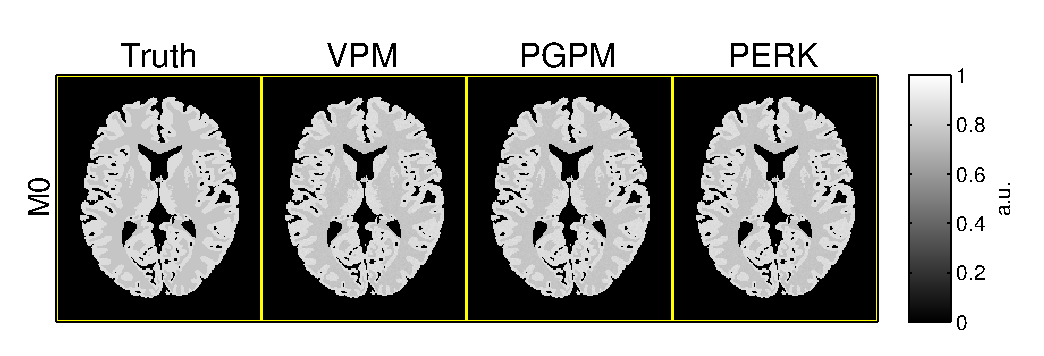
\includegraphics [width=0.99\textwidth] {%
			sim/sp2de1,sl-81,m0,im,gray.eps%
		}
		\label{fig:perk,sim,m0,im,gray}
	}
	\hspace{0cm}
	\subfigure{%
		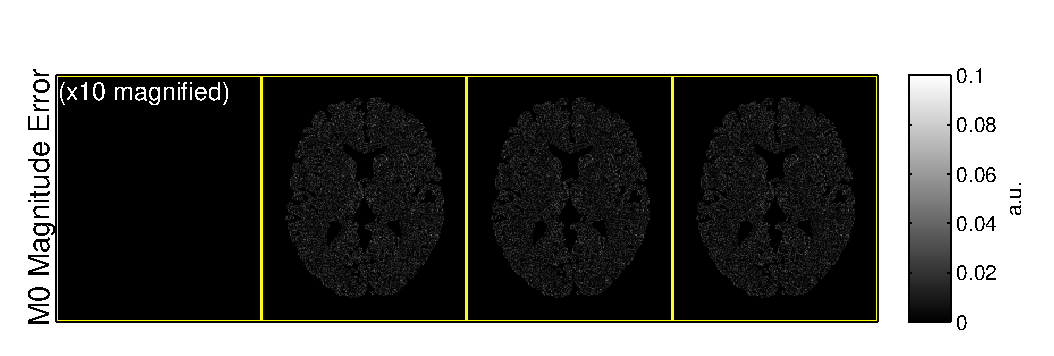
\includegraphics [width=\textwidth,trim=0 0 0 25,clip] {%
			sim/sp2de1,sl-81,m0,err,gray.eps%
		}
		\label{fig:perk,sim,m0,err,gray}
	}
	\caption{%
		$\mzero$ VPM, PGPM, and PERK estimates
		and corresponding error images,
		in simulation.
		Magnitude error images are $10\times$ magnified.
		Voxels not assigned WM- or GM-like relaxation times
		are masked out in post-processing for display.
		Difference images demonstrate
		that all three $\mzero$ estimates
		exhibit low estimation error.
		Table~\ref{tab:perk,sim} presents
		corresponding sample statistics.
	}
	\label{fig:perk,sim,m0}
\end{figure}
	
\begin{figure}[!ht]
	\centering
	\subfigure{%
		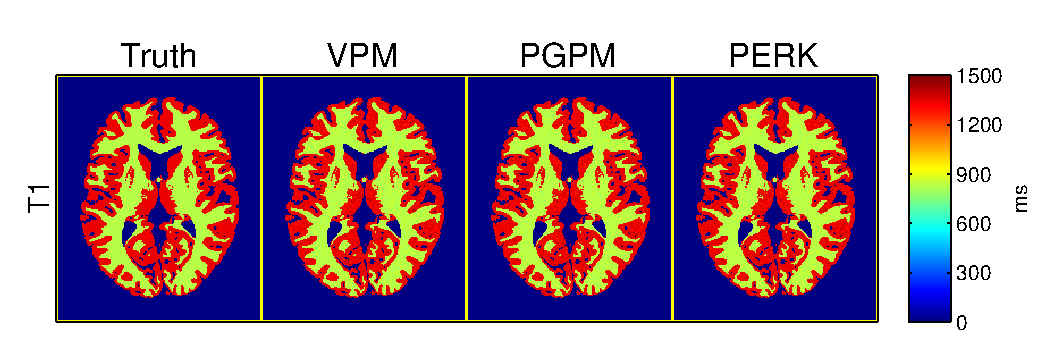
\includegraphics [width=\textwidth] {%
			sim/sp2de1,sl-81,t1,im,jet.eps%
		}
		\label{fig:perk,sim,t1,im,jet}
	}
	\hspace{0cm}
	\subfigure{%
		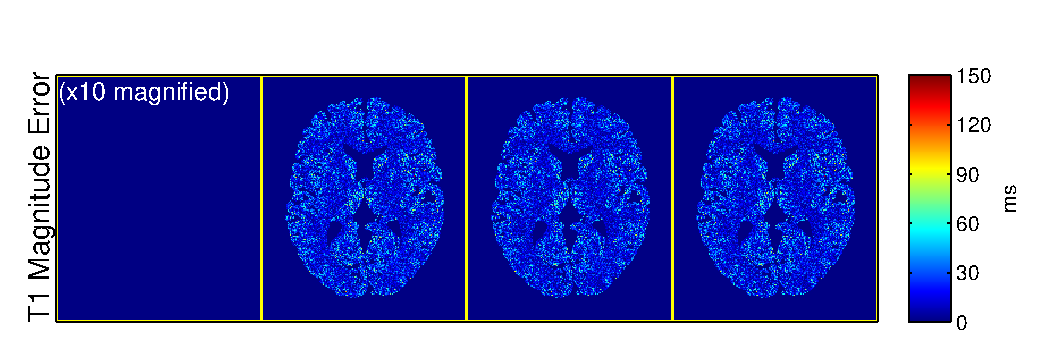
\includegraphics [width=0.99\textwidth,trim=0 0 0 25,clip] {%
			sim/sp2de1,sl-81,t1,err,jet.eps%
		}
		\label{fig:perk,sim,t1,err,jet}
	}
	\caption{%
		$\To$	VPM, PGPM, and PERK estimates
		and corresponding error images,
		in simulation.
		Magnitude error images are $10\times$ magnified.
		Voxels not assigned WM- or GM-like relaxation times
		are masked out in post-processing for display.
		Difference images demonstrate
		that all three $\To$ estimates
		exhibit low estimation error.
		Table~\ref{tab:perk,sim} presents
		corresponding sample statistics.
	}
	\label{fig:perk,sim,t1}
\end{figure}

\begin{figure}[!ht]
	\centering
	\subfigure{%
		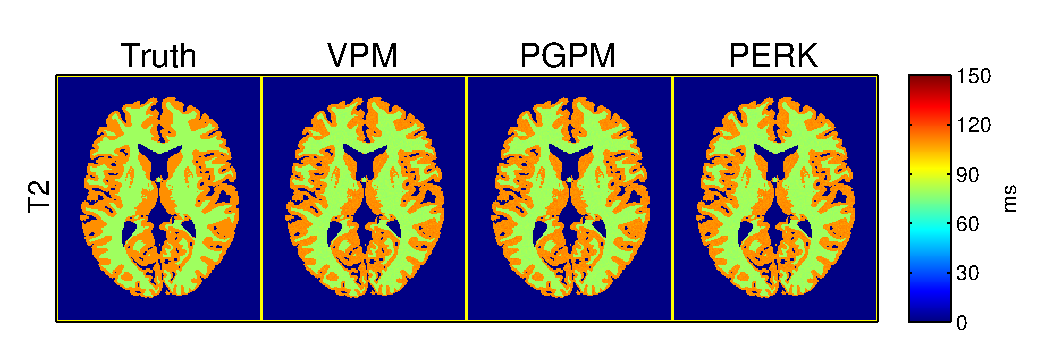
\includegraphics [width=\textwidth] {%
			sim/sp2de1,sl-81,t2,im,jet.eps%
		}
		\label{fig:perk,sim,t2,im,jet}
	}
	\hspace{0cm}
	\subfigure{%
		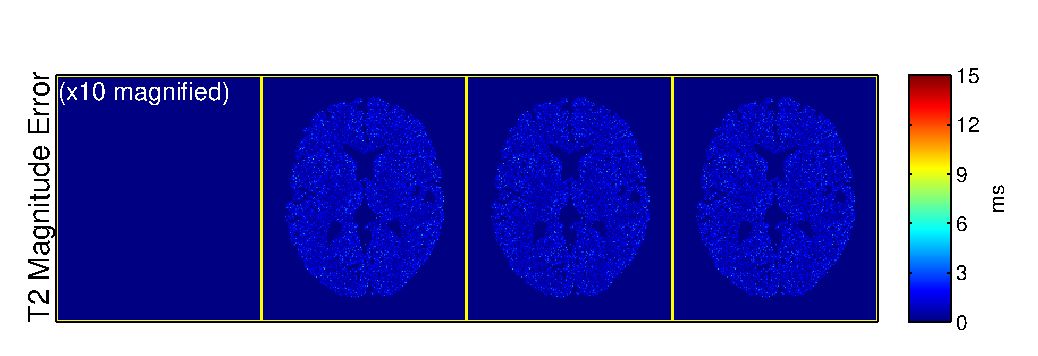
\includegraphics [width=0.99\textwidth,trim=0 0 0 25,clip] {%
			sim/sp2de1,sl-81,t2,err,jet.eps%
		}
		\label{fig:perk,sim,t2,err,jet}
	}
	\caption{%
		$\Tt$ VPM, PGPM, and PERK estimates
		and corresponding error images,
		in simulation.
		Magnitude error images are $10\times$ magnified.
		Voxels not assigned WM- or GM-like relaxation times
		are masked out in post-processing for display.
		Difference images demonstrate
		that all three $\To$ estimates
		exhibit low estimation error.
		Table~\ref{tab:perk,sim} presents
		corresponding sample statistics.
	}
	\label{fig:perk,sim,t2}
\end{figure}

Figs.~\ref{fig:perk,sim,m0}, \ref{fig:perk,sim,t1}, and \ref{fig:perk,sim,t2}
compare VPM, PGPM, and PERK estimates
of $\mzero$, $\To$, $\Tt$ respectively,
alongside $10\times$ magnified absolute difference images 
with respect to the ground truth.
Voxels not assigned WM- or GM-like relaxation times
are masked out in post-processing for display.
Difference images demonstrate
that within WM- and GM-like voxels,
all three methods exhibit low estimation error.

\begin{table}[!ht]
	\footnotesize
	\centering
	\begin{tabular}{c | r | r r r}
		\hline
		\hline
								& Truth 	& VPM 													
													& PGPM 																	& PERK \\
		\hline
		WM $\mzero$	& $0.77$	& \mnstd{0.7700}{0.00919} $(0.0092)$ 
													& \mnstd{0.76999}{0.00871} $(0.00871)$ 	& \mnstd{0.77002}{0.00873} $(0.00873)$ \\
		GM $\mzero$	& $0.86$	& \mnstd{0.8601}{0.01192} $(0.0119)$
													& \mnstd{0.8600}{0.01142} $(0.0114)$ 		& \mnstd{0.8613}{0.01147} $(0.0133)$ \\
		\hline
		WM $\To$ 		& $832$ 	& \mnstd{832.1}{17.2} $(17.2)$	
													& \mnstd{832.1}{16.2} $(16.2)$ 					& \mnstd{833.0}{16.5} $(16.5)$ \\
		GM $\To$ 		& $1331$ 	& \mnstd{1331.5}{31.1} $(31.1)$ 
													& \mnstd{1331.2}{29.7} $(29.7)$ 				& \mnstd{1332.1}{30.4} $(30.4)$ \\ 
		\hline
		WM $\Tt$ 		& $79.6$	& \mnstd{79.61}{0.988} $(0.988)$
													& \mnstd{79.60}{0.952} $(0.952)$ 				& \mnstd{79.46}{0.978} $(0.989)$ \\
		GM $\Tt$ 		& $110.$ 	& \mnstd{110.02}{1.40} $(1.40)$
													& \mnstd{110.02}{1.35} $(1.35)$ 				& \mnstd{109.91}{1.35} $(1.35)$ \\
    \hline
    \hline
  \end{tabular}
  \caption{%
  	Sample means $\pm$ sample standard deviations (RMSEs)
		of VPM, PGPM, and PERK $\mzero,\To,\Tt$ estimates,
		computed in simulation
		over $7810$ WM-like and $9162$ GM-like voxels.
		Each sample statistic is rounded off
		to the highest place value
		of its (unreported) standard error,
		computed via formulas in \cite{ahn:03:seo}.
		$\mzero$ values are unitless.
		$\To,\Tt$ values are in milliseconds.
		Figs.~\ref{fig:perk,sim,m0}, \ref{fig:perk,sim,t1}, and \ref{fig:perk,sim,t2}
		present corresponding images.
	}
	\label{tab:perk,sim}
\end{table}

Table~\ref{tab:perk,sim} compares sample statistics
of VPM, PGPM, and PERK $\mzero,\To,\Tt$ estimates,
computed over $7810$ WM-like and $9162$ GM-like voxels.
Overall,
all three methods achieve excellent performance.
PERK estimates are slightly more precise 
but slightly less accurate 
than gold-standard VPM estimates. 
Results suggest that 
at least in WM- and GM-like voxels,
PGPM is capable of descending the ML cost 
towards a desirable solution;
in fact, PGPM achieves slightly better precision
than either VPM or PERK.
All three methods exhibit comparable 
root mean squared errors (RMSEs).

%%%%%%%%%%%%%%%%%%%%%%%%%%%%%%%%%%%%%%%%%%%%%%%%%%%
\subsection{Phantom Experiments}
\label{ss,perk,exp,phant}

\begin{figure}[!t]
	\centering
	\begin{minipage}{\textwidth}
  	\subfigure{%
  		\includegraphics [width=0.96\textwidth] {%
  			hpd-tight/sp2de1,sl-6,m0,im-gray.eps%
  		}
  		\label{fig:perk,hpd-tight,m0,im-gray}
  	}
  	\hspace{0cm}
  	\subfigure{%
  		\includegraphics [width=0.982\textwidth,trim=0 0 0 25,clip] {%
  			hpd-tight/sp2de1,sl-6,t1,im-jet.eps%
  		}
  		\label{fig:perk,hpd-tight,t1,im-jet}
  	}
  	\hspace{0cm}
  	\subfigure{%
  		\includegraphics [width=0.97\textwidth,trim=0 0 0 25,clip] {%
  			hpd-tight/sp2de1,sl-6,t2,im-jet.eps%
  		}
  		\label{fig:perk,hpd-tight,t2,im-jet}
  	}
	\end{minipage}
	\caption{%
		VPM, PGPM, and PERK $\mzero,\To,\Tt$ estimates 
		in a quantitative phantom.
		Vials are enumerated and highlighted
		to correspond with markers and colored boxes
		in Fig.~\ref{fig:perk,hpd-tight,plot}.
		PERK has only been trained 
		to accurately estimate within vials 4-8;
		within these vials,
		VPM, PGPM, and PERK estimates 
		appear visually similar.
	}
	\label{fig:perk,hpd-tight}
\end{figure}

\begin{figure*}[!t]
	\centering
	\subfigure{%
		\includegraphics [width=0.47\textwidth]{%
			hpd-tight/sp2de1,sl-6,t1,plot%
		}
		\label{fig:perk,hpd-tight,t1,plot}
	}
	\hspace{0.3cm}
	\subfigure{%
		\includegraphics [width=0.47\textwidth] {%
			hpd-tight/sp2de1,sl-6,t2,plot%
		}
		\label{fig:perk,hpd-tight,t2,plot}
	}
	\vspace{0.3cm}
	\begin{tabular}{c || r | r r r}
		\hline
		\hline
		 					& NMR										& VPM 							& PGPM									& PERK \\
		\hline
		V4 $\To$	& \mnstd{1604}{7.2} 		& \mnstd{1645}{48} 	& \mnstd{1649}{48}			& \mnstd{1626}{46} 	\\        
    V5 $\To$	& \mnstd{1332}{0.8} 		& \mnstd{1335}{61} 	& \mnstd{1331}{41}			& \mnstd{1332}{40.} \\        
    V6 $\To$	& \mnstd{1044}{3.2} 		& \mnstd{1055}{28} 	& \mnstd{1060.}{29}			& \mnstd{1061}{29} 	\\        
    V7 $\To$	& \mnstd{801.7}{1.70}		& \mnstd{834}{21} 	& \mnstd{840.}{23}			& \mnstd{839}{23} 	\\         
    V8 $\To$	& \mnstd{608.6}{1.03} 	& \mnstd{627}{25} 	& \mnstd{623}{12}				& \mnstd{620.}{13} 	\\    
		\hline
		\hline
		V4 $\Tt$	& \mnstd{190.94}{0.011}	&	\mnstd{194}{5.5}	& \mnstd{192.4}{5.2}		& \mnstd{192.5}{4.9}\\    
    V5 $\Tt$	& \mnstd{133.27}{0.073} &	\mnstd{131.2}{5.3}& \mnstd{131}{5.5} 			& \mnstd{131}{5.5}  \\       
    V6 $\Tt$	& \mnstd{96.89}{0.049}  &	\mnstd{90.8}{3.5} & \mnstd{90.8}{3.5}			& \mnstd{90.9}{3.5} \\         
    V7 $\Tt$	& \mnstd{64.07}{0.034}  &	\mnstd{64.6}{2.2} & \mnstd{64.5}{2.1} 		& \mnstd{65.0}{2.1} \\        
    V8 $\Tt$	& \mnstd{46.42}{0.014}  &	\mnstd{46.4}{1.5} & \mnstd{46.4}{1.5} 		& \mnstd{46.1}{1.5} \\   
		\hline
		\hline
	\end{tabular}
	\caption{%
		Phantom sample statistics
		of VPM, PGPM, and PERK $\To,\Tt$ estimates
		and NIST NMR reference measurements \cite{keenan:16:msm}.
		Plot markers and error bars indicate sample means
		and sample standard deviations
		computed over ROIs
		within the 14 vials
		labeled and color-coded 
		in Fig.~\ref{fig:perk,hpd-tight}.
		Yellow box boundaries 
		indicate projections
		of the PERK sampling distribution's support $\supp{\dist{\bmx,\bmnu}}$.
		Missing markers lie outside axis limits.
		Corresponding tables replicate 
		sample means $\pm$ sample standard deviations
		for vials within $\supp{\dist{\bmx,\bmnu}}$.
		Each value is rounded off
		to the highest place value 
		of its (unreported) standard error,
		computed via formulas in \cite{ahn:03:seo}.
		`V\#' indicates vial numbers.
		All values are reported in milliseconds.
		Within $\supp{\dist{\bmx,\bmnu}}$, 
		VPM, PGPM, and PERK estimates agree excellently 
		with each other
		and reasonably with NMR measurements.
	}
	\label{fig:perk,hpd-tight,plot}
\end{figure*}		 

Phantom experiments used datasets 
from fast coronal scans
of a High Precision Devices\regis MR system phantom $\Tt$ array
acquired on a 3T GE Discovery\tmark scanner
with an 8-channel receive head array.
This acquisition consisted of: 
two SPGR scans 
with $5,15^\circ$ flip angles
and $12.2,12.2$ms repetition times;
one DESS scan 
with $30^\circ$ flip angle
and $17.5$ms repetition time;
and two Bloch-Siegert (BS) scans \cite{sacolick:10:bmb}
(for separate flip angle scaling estimation).
Nominal flip angles were achieved 
by scaling a 2cm slab-selective Shinnar-Le Roux RF pulse \cite{pauly:91:prf}
of duration 1.28ms and time-bandwidth product 4.
All scans collected fully-sampled 3D Cartesian data
using 4.67ms echo times
with a $256\times256\times8$ matrix
over a $24\times24\times4$cm$^3$ field of view. 
Scan time totaled 3m17s. 
The scan room temperature was recorded as $293$K
at the beginning of the exam. 
Further acquisition details are in \cite{nataraj:17:oms}.

For each SPGR, DESS, and BS dataset, 
we reconstructed raw coil images via 3D Fourier transform
and subsequently processed only one image slice
centered within the excitation slab.
We combined SPGR and DESS coil images 
using a natural extension of \cite{ying:07:jir}
to the case of multiple datasets.
We similarly (but separately) combined BS coil images
and estimated $\kappa$ maps
by normalizing and calibrating
regularized transmit field estimates \cite{sun:14:reo}
from complex coil-combined BS images.
We estimated $\mzero,\To,\Tt$
from magnitude SPGR/DESS images and $\kappa$ maps
using VPM, PGPM, and PERK.
VPM took 928s;
PGPM took 1257s; 
and PERK training and testing
respectively took 4.2s and 1.9s.

Fig.~\ref{fig:perk,hpd-tight} compares
VPM, PGPM, and PERK $\mzero,\To,\Tt$ estimates.
Vials are enumerated in descending $\To,\Tt$ order.
Vials whose $\To,\Tt$ values
are within sampling distribution support $\supp{\dist{\bmx,\bmnu}}$
(as measured by NIST NMR reference measurements \cite{keenan:16:msm})
have labels highlighted
with yellow numbers.
Here, 
$\supp{\dist{\bmx,\bmnu}}$ was chosen 
to reflect the ranges of latent parameter values
for which the SPGR/DESS scan parameters 
were optimized in \cite{nataraj:17:oms}.
Circular ROIs are selected well away from vial encasings
and correspond with sample statistics 
presented in Fig.~\ref{fig:perk,hpd-tight,plot}.                                                                                                                                                                                 
Distilled water surrounds the encased vials.
Within the highlighted vials of interest,
VPM, PGPM, and PERK estimates 
appear visually similar.

Fig.~\ref{fig:perk,hpd-tight,plot} compares
sample means and sample standard deviations
computed within ROIs 
of VPM, PGPM, and PERK $\To,\Tt$ estimates
against nuclear magnetic resonance (NMR) reference measurements 
reported at 293.00K
from the National Institute 
for Standards of Technology (NIST) \cite{keenan:16:msm}.
Yellow box boundaries indicate projections
of the PERK sampling distribution's support $\supp{\dist{\bmx,\bmnu}}$.
ROI labels correspond with vial markers
depicted in Fig.~\ref{fig:perk,hpd-tight}.
Within $\supp{\dist{\bmx,\bmnu}}$,
corresponding tables demonstrate
that VPM, PGPM, and PERK estimates agree excellently 
with each other 
and reasonably with NMR measurements.
We do not expect good PERK performance
outside $\supp{\dist{\bmx,\bmnu}}$ 
and indeed observe 
poor ability to extrapolate.
As discussed in Subsection~\ref{sss,perk,pract,mod,dist}
and demonstrated in Subsection~\ref{ss,perk,robust,dist},
expanding $\supp{\dist{\bmx,\bmnu}}$
well beyond the acquisition design 
parameter range of interest
can reduce PERK performance
for typical $\To,\Tt$ WM and GM values.

%%%%%%%%%%%%%%%%%%%%%%%%%%%%%%%%%%%%%%%%%%%%%%%%%%%
\subsection{\Invivo Experiments}
\label{ss,perk,exp,invivo}

\Invivo experiments used datasets
from axial scans of a healthy volunteer
acquired with a 32-channel Nova Medical\regis receive head array.
To address bulk motion between scans,
we rigidly registered coil-combined images 
to a reference
before parameter estimation.
All other data acquisition, 
image reconstruction, 
and parameter estimation details
are the same as in phantom experiments
(acquisition and reconstruction details 
are reported in \cite{nataraj:17:oms}).
VPM took 838s;
PGPM took 2178s;
and PERK training and testing
took 4.2s and 1.6s.

\begin{figure*}[!ht]
	\centering
	\begin{minipage}{\textwidth}
  	\subfigure{%
  		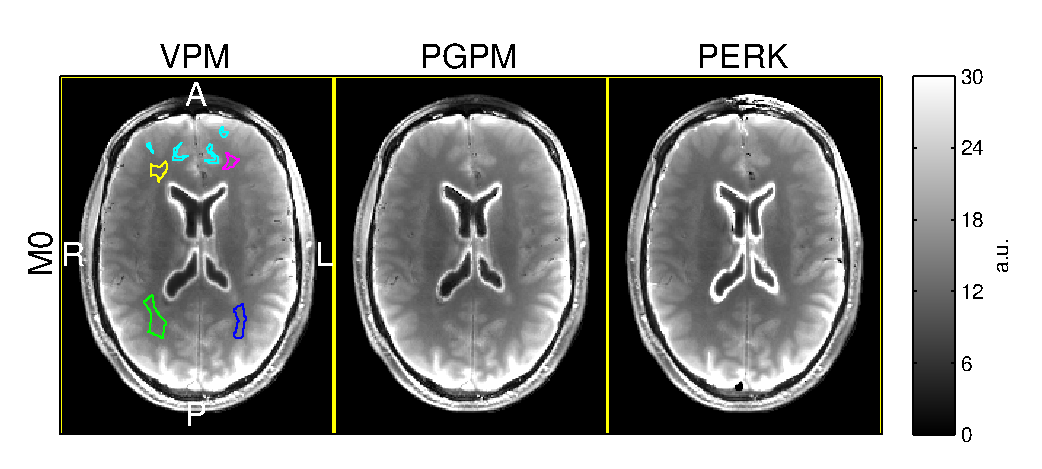
\includegraphics [width=0.96\textwidth,trim=0 0 0 10,clip] {%
  			brain/sp2de1,sl-5,m0,im-gray.eps%
  		}%
  		\label{fig:perk,brain,m0,im-gray}
  	}%
  	\hspace{0cm}
  	\subfigure{%
  		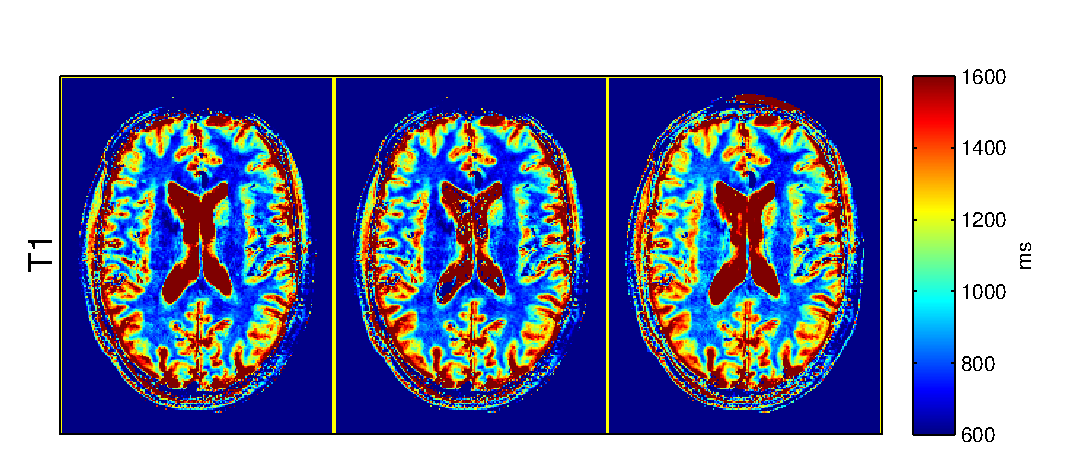
\includegraphics [width=0.982\textwidth,trim=0 0 0 20,clip] {%
  			brain/sp2de1,sl-5,t1,im-jet.eps%
  		}
  		\label{fig:perk,brain,t1,im-jet}
  	}%
  	\hspace{0cm}
  	\subfigure{%
  		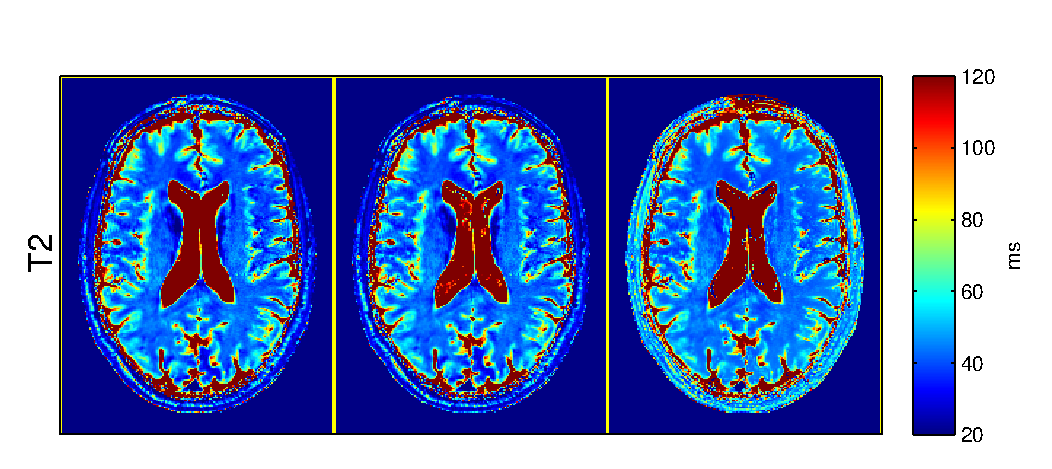
\includegraphics [width=0.97\textwidth,trim=0 0 0 20,clip] {%
  			brain/sp2de1,sl-5,t2,im-jet.eps%
  		}%
  		\label{fig:perk,brain,t2,im-jet}
  	}%
	\end{minipage}
	\caption{%
		VPM, PGPM and PERK estimates
		of $\mzero,\To,\Tt$ 
		in the brain of a healthy volunteer.
		Separate WM ROIs are distinguished
		by anterior/posterior (A/P)
		and right/left (R/L) directions.
		Four small anterior cortical GM polygons
		are pooled into a single GM ROI.
		Images are cropped in post-processing 
		for display.
	}
	\label{fig:perk,brain}
\end{figure*}

\begin{table}[!ht]
	\centering
	\begin{tabular}{r | c | r r r}
		\hline
		\hline
			& ROI 		& VPM 							& PGPM 							& PERK 									\\
		\hline
		\multirow{5}{*}{$\To$}
			& \AR WM 	& \mnstd{778}{28}		& \mnstd{779}{27}		& \mnstd{832}{31} 			\\
      & \AL WM 	& \mnstd{731}{37}   & \mnstd{713}{33}		& \mnstd{725}{41}				\\
      & \PR WM 	& \mnstd{805}{52}   & \mnstd{796}{51}		& \mnstd{831}{51}				\\
      & \PL WM 	& \mnstd{789}{40}   & \mnstd{788}{38} 	& \mnstd{815}{42}				\\
      & \A 	GM 	& \mnstd{1120}{180} & \mnstd{1120}{180}	& \mnstd{1150}{170.}		\\
    \hline
    \multirow{5}{*}{$\Tt$}
      & \AR WM 	&	\mnstd{40.0}{1.29}& \mnstd{40.0}{1.27}& \mnstd{41.18}{0.94} 	\\
      & \AL WM 	& \mnstd{39.7}{1.7} & \mnstd{39.7}{1.7}	& \mnstd{41.3}{1.02}		\\
      & \PR WM	& \mnstd{43.0}{2.7} & \mnstd{43.0}{2.7} & \mnstd{43.7}{2.6}			\\
      & \PL WM 	&	\mnstd{43.0}{1.8} &	\mnstd{43.0}{1.8} & \mnstd{43.5}{1.36}		\\
      & \A 	GM	& \mnstd{53.5}{11.8}&	\mnstd{53.4}{11.7}& \mnstd{53.3}{11.6}		\\
   	\hline
		\hline
	\end{tabular}
	\caption{%
		\Invivo sample means $\pm$ sample standard deviations
		of VPM, PGPM, and PERK $\To,\Tt$ estimates,
		computed over color-coded ROIs
		indicated in Fig.~\ref{fig:perk,brain}.
		Each value is rounded off 
		to the highest place value
		of its (unreported) standard error,
		computed via formulas in \cite{ahn:03:seo}.
		All values are in milliseconds.
	}
	\label{tab:perk,brain}
\end{table}

Fig.~\ref{fig:perk,brain} compares 
VPM, PGPM, and PERK $\mzero,\To,\Tt$ estimates.
The PERK $\mzero$ estimate appears smoothed
(although no spatial regularization was used)
but is otherwise very similar
to the VPM and PGPM $\mzero$ estimates.
Narrow display ranges emphasize
that VPM, PGPM, and PERK $\To,\Tt$ estimates 
discern cortical WM/GM boundaries similarly,
though PERK $\To$ estimates are noticeably highest
in some WM regions.
VPM, PGPM, and PERK $\Tt$ estimates are nearly indistinguishable 
in lateral regions
but disagree somewhat 
in medial regions close 
to cerebrospinal fluid (CSF).
We neither expect nor observe reasonable PERK performance
in voxels containing CSF.

Table~\ref{tab:perk,brain} summarizes sample statistics
of VPM, PGPM, and PERK $\To,\Tt$ estimates,
computed over four separate WM ROIs 
containing $96$, $69$, $224$, and $148$ voxels
and one pooled cortical anterior GM ROI 
containing $156$ voxels.
Overall,
VPM, PGPM, and PERK $\To,\Tt$ estimates are comparable.
$\To$ estimates in GM
and $\Tt$ estimates in WM/GM
do not differ significantly.
PERK $\To$ estimates are significantly higher
than VPM and PGPM $\To$ estimates 
in one WM ROI;
however,
all $\To$ estimates 
are well within the range 
of typical literature measurements at 3T 
(see \eg \cite{wansapura:99:nrt, stanisz:05:ttr}).

%%%%%%%%%%%%%%%%%%%%%%%%%%%%%%%%%%%%%%%%%%%%%%%%%%%
\section{Robustness Studies}
\label{s,perk,robust}
%%%%%%%%%%%%%%%%%%%%%%%%%%%%%%%%%%%%%%%%%%%%%%%%%%%

This section investigates PERK robustness
to two types of non-idealities
that may be encountered 
in other applications.
Subsection~\ref{ss,perk,robust,noise} 
studies PERK performance sensitivity
to mismatch between training and testing noise variance.
Subsection~\ref{ss,perk,robust,dist}
studies PERK performance degradation
when trained 
with latent parameter distributions
that have wider support
than the parameter ranges
used for optimizing the scan design
in \cite{nataraj:17:oms}.

%%%%%%%%%%%%%%%%%%%%%%%%%%%%%%%%%%%%%%%%%%%%%%%%%%%
\subsection{Mismatch in Training vs. Testing Noise Statistics}
\label{ss,perk,robust,noise}

\begin{figure}[!t]
	\centering
	\subfigure{%
		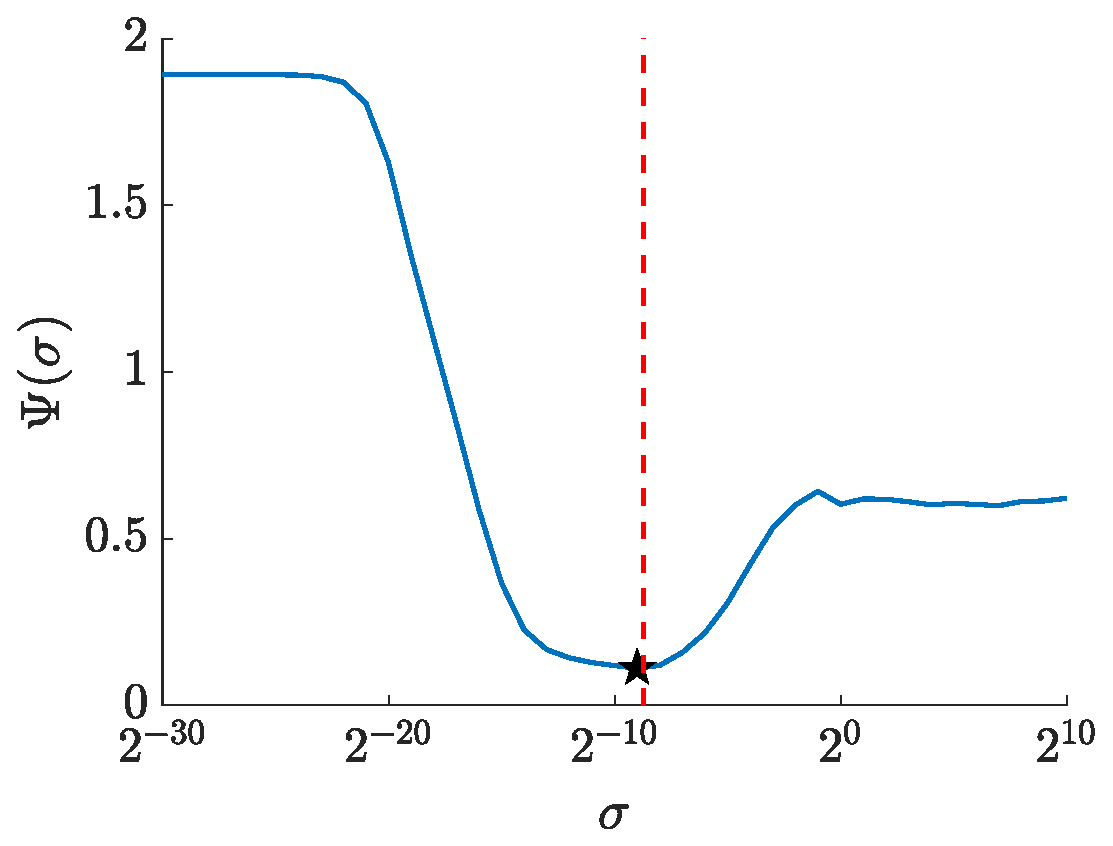
\includegraphics [width=0.47\textwidth] {%
			tune/robust,broad,w-t12.eps%
		}
		\label{fig:perk,robust,broad}
	}
	\hspace{0cm}
	\subfigure{%
		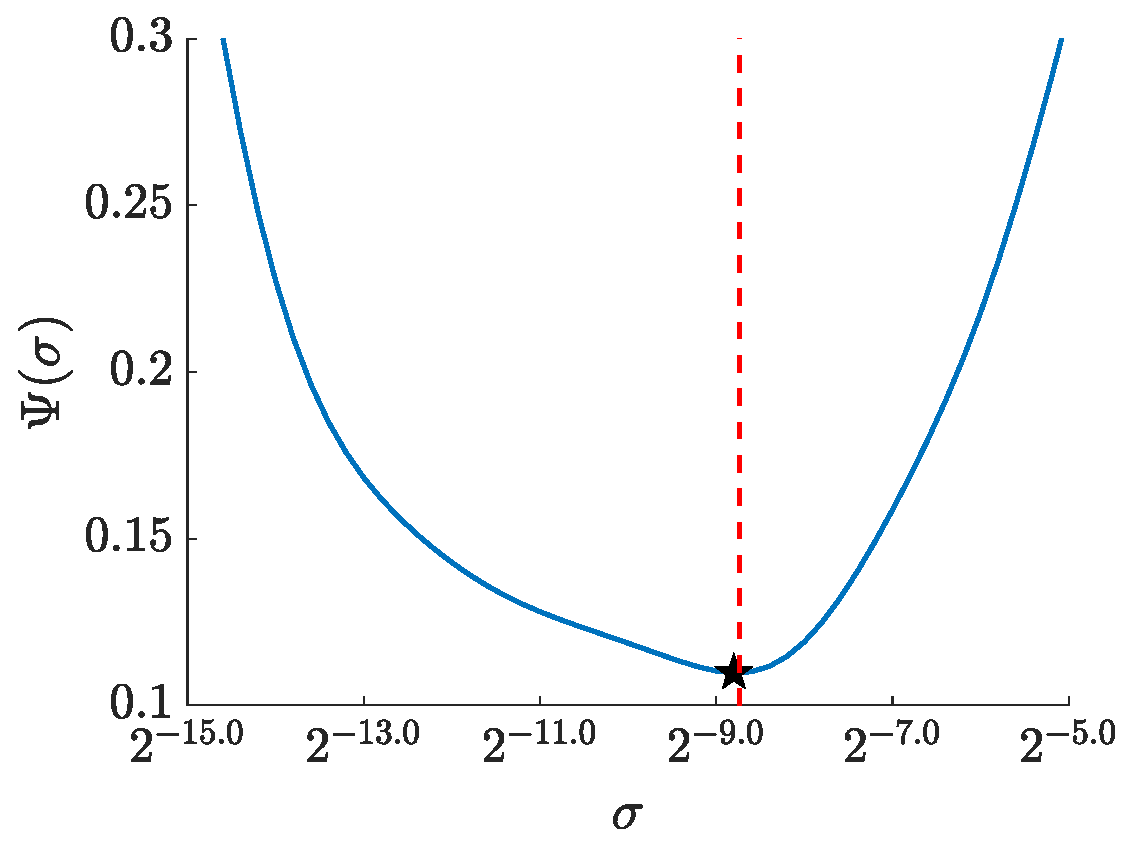
\includegraphics [width=0.47\textwidth] {%
			tune/robust,tight,w-t12.eps%
		}
		\label{fig:perk,robust,tight}
	}
	\caption{%
		Performance criterion $\costa{\sigma}$
		versus PERK training noise standard deviation $\sigma$,
		over two different scales.
		Similar to Fig.~\ref{fig:perk,holdout},
		each point on the blue curve
		is the weighted normalized root mean squared error
		of a separately trained PERK estimator.
		In each subplot,
		a black star marks 
		the performance criterion minimizer
		$\est{\sigma} \gets 2^{-8.8}$
		while a dashed red line
		marks the (latent) test data noise standard deviation 
		$\sigma^\star \gets 2^{-8.736}$.
		To within quantization error,
		PERK performs best 
		when trained with training data
		whose noise statistics 
		match test data noise statistics.
		Performance degradation as measured by $\cost$ 
		does not exceed $10\%$
		for $\sigma$ values within a factor of two
		of $\sigma^\star$.
		This result suggests 
		that PERK is somewhat robust
		to moderate misspecification of the noise level.
	}%
	\label{fig:perk,robust}
\end{figure}

To assess the importance
of training PERK
with appropriately noisy training data,
we investigated PERK's performance sensitivity
to the standard deviation $\sigma$
of the noise distribution 
from which noise realizations are drawn
to generate training data.
Instead of setting $\sigma$ online
as in other experiments,
here we fixed $\sigma$ offline
to one of many discretized values
spanning many orders of magnitude.
Otherwise as described 
in Subsection~\ref{ss,perk,exp,meth},
we trained a PERK estimator
for each $\sigma$ setting.
Similar to Subsection~\ref{sss,perk,exp,meth,holdout},
we tested each PERK estimator 
on a separate simulated dataset
consisting of $10^5$ samples 
from training prior distribution $\dist{\bmx,\bmnu}$.
We assessed performance sensitivity
by comparing evaluations $\costa{\sigma}$ 
of holdout cost \eqref{eq:perk,holdout}
at each $\sigma$ setting.
	
Fig.~\ref{fig:perk,robust} plots $\costa{\sigma}$
as $\sigma$ is varied 
over two different scales.
In each subplot,
a black star marks the minimizer 
$\hat{\sigma} \gets 2^{-8.8}$
while a dashed red line marks
the (latent) test data noise standard deviation 
$\sigma^\star \gets 2^{-8.736}$.
To within quantization error,
PERK performs best 
when trained with training data
whose noise statistics 
match test data noise statistics.
As measured by $\cost$, 
PERK performance degrades by at most $10\%$ 
for choices of $\sigma \in \brac{2^{-10.2},2^{-8}}$.
Results suggest
that for good PERK performance,
it is desirable
to set $\sigma$
to within about a factor of two
of the test data noise standard deviation $\sigma^\star$.
Nevertheless,
there is a zone near $\sigma^\star$
where PERK performance is reasonably similar,
indicating that PERK is somewhat robust
to some misspecification of the noise level.

%%%%%%%%%%%%%%%%%%%%%%%%%%%%%%%%%%%%%%%%%%%%%%%%%%%
\subsection{Mismatch in Scan Design vs. Sampling Distribution Support}
\label{ss,perk,robust,dist}

Although the SPGR/DESS acquisition
was optimized in \cite{nataraj:17:oms}
for a certain range of $\To,\Tt$ values,
it is interesting to investigate
how well PERK can perform 
outside that parameter range
if presented (simulated) training data
over a wider range of latent parameters.
It is also interesting to explore
whether using such a wider range 
of latent parameters for training
degrades performance
for the parameter range 
of primary interest.
Thus, 
we repeated the phantom experiment
described in Subsection~\ref{ss,perk,exp,phant}
except now using a PERK estimator
trained using a sampling prior distribution
with broader support.
We still assume a separable prior distribution
$\dist{\bmx,\bmnu} \gets \dist{\mzero}\dist{\To}\dist{\Tt}\dist{\kappa}$ 
(with $\dist{\mzero}$ and $\dist{\kappa}$ set as before)
but now set 
$\dist{\To} \gets \logunif{10^{1.5}, 10^{3.5}}$ 
and 
$\dist{\Tt} \gets \logunif{10^{0.5}, 10^{3.5}}$ 
to have wider supports.
These support endpoints 
now match the grid search support
used by the VPM.
All other training and testing details are unchanged from before.

\begin{figure*}[!t]
	\centering
	\subfigure{%
		\includegraphics [width=0.47\textwidth]{%
			hpd-broad/sp2de1,sl-6,t1,plot%
		}
		\label{fig:perk,hpd-broad,t1,plot}
	}
	\hspace{0.3cm}
	\subfigure{%
		\includegraphics [width=0.47\textwidth] {%
			hpd-broad/sp2de1,sl-6,t2,plot%
		}
		\label{fig:perk,hpd-broad,t2,plot}
	}
	\vspace{0.3cm}
	\begin{tabular}{c || r | r r r}
		\hline
		\hline
		 					& NMR										& VPM 							& PGPM 									& PERK 								\\
		\hline
		V4 $\To$	& \mnstd{1604}{7.2} 		& \mnstd{1645}{48} 	& \mnstd{1639}{48}			& \mnstd{1649}{51} 		\\        
    V5 $\To$	& \mnstd{1332}{0.8} 		& \mnstd{1335}{61} 	& \mnstd{1331}{41}			& \mnstd{1343}{40.} 	\\        
    V6 $\To$	& \mnstd{1044}{3.2} 		& \mnstd{1055}{28} 	& \mnstd{1060.}{29}			& \mnstd{1083}{32} 		\\        
    V7 $\To$	& \mnstd{801.7}{1.70}		& \mnstd{834}{21} 	& \mnstd{840.}{23}			& \mnstd{821}{25} 		\\         
    V8 $\To$	& \mnstd{608.6}{1.03} 	& \mnstd{627}{25} 	& \mnstd{623}{12}				& \mnstd{604}{18} 		\\  
		\hline
		\hline
		V4 $\Tt$	& \mnstd{190.94}{0.011}	&	\mnstd{194}{5.5}	& \mnstd{193.1}{5.2}		& \mnstd{197}{11}			\\    
    V5 $\Tt$	& \mnstd{133.27}{0.073} &	\mnstd{131.2}{5.3}& \mnstd{131}{5.5} 			& \mnstd{138}{8}  		\\       
    V6 $\Tt$	& \mnstd{96.89}{0.049}  &	\mnstd{90.8}{3.5} & \mnstd{90.8}{3.5}			& \mnstd{106.6}{3.6} 	\\         
    V7 $\Tt$	& \mnstd{64.07}{0.034}  &	\mnstd{64.6}{2.2} & \mnstd{64.5}{2.1} 		& \mnstd{89.2}{3.7} 	\\        
    V8 $\Tt$	& \mnstd{46.42}{0.014}  &	\mnstd{46.4}{1.5} & \mnstd{46.4}{1.5} 		& \mnstd{48.9}{4.6} 	\\
    \hline
    \hline      
	\end{tabular}
	\caption{%
		Phantom sample statistics
		of more aggressively trained 
		VPM, PGPM, and PERK $\To,\Tt$ estimates
		and NIST NMR reference measurements \cite{keenan:16:msm}.
		Unlike analogous results in Fig.~\ref{fig:perk,hpd-tight,plot},
		here the PERK estimator was trained
		with a sampling distribution
		whose support extended 
		well beyond the range of $\To,\Tt$ values
		for which the acquisition was optimized 
		in \cite{nataraj:17:oms}.
		Comparing to Fig.~\ref{fig:perk,hpd-tight,plot},
		we find that PERK estimator performance degrades 
		within the highlighted $\To,\Tt$ range of interest.
		Plot markers and error bars
		indicate sample means and sample standard deviations
		computed over ROIs
		within the 14 vials
		labeled and color-coded
		in Fig.~\ref{fig:perk,hpd-broad}.
		Corresponding tables replicate 
		sample means $\pm$ sample standard deviations
		for vials within the highlighted range.
		Each value is rounded off
		to the highest place value 
		of its (unreported) standard error,
		computed via formulas in \cite{ahn:03:seo}.
		All values are in milliseconds.
	}
	\label{fig:perk,hpd-broad,plot}
\end{figure*}

\begin{figure}[!t]
	\centering
	\begin{minipage}{\textwidth}
  	\subfigure{%
  		\includegraphics [width=0.96\textwidth] {%
  			hpd-broad/sp2de1,sl-6,m0,im-gray.eps%
  		}
  		\label{fig:perk,hpd-broad,m0,im-gray}
  	}
  	\hspace{0cm}
  	\subfigure{%
  		\includegraphics [width=0.982\textwidth,trim=0 0 0 25,clip] {%
  			hpd-broad/sp2de1,sl-6,t1,im-jet.eps%
  		}
  		\label{fig:perk,hpd-broad,t1,im-jet}
  	}
  	\hspace{0cm}
  	\subfigure{%
  		\includegraphics [width=0.97\textwidth,trim=0 0 0 25,clip] {%
  			hpd-broad/sp2de1,sl-6,t2,im-jet.eps%
  		}
  		\label{fig:perk,hpd-broad,t2,im-jet}
  	}
	\end{minipage}
	\caption{%
		More aggressively trained 
		VPM, PGPM, and PERK $\mzero,\To,\Tt$ estimates
		in a quantitative phantom.
		Here the PERK estimator was trained
		with a sampling distribution
		whose support extended
		over less well identified $\To,\Tt$ values.
		Comparing with analogous images 
		in Fig.~\ref{fig:perk,hpd-tight},
		PERK performance within vials 4-8 degrades,
		though in other vials 
		performance clearly improves. 
		Vials are enumerated and highlighted
		to correspond with markers and colored boxes
		in Fig.~\ref{fig:perk,hpd-broad,plot}.
	}
	\label{fig:perk,hpd-broad}
\end{figure}

Fig.~\ref{fig:perk,hpd-broad,plot} 
is analogous to Fig.~\ref{fig:perk,hpd-tight,plot}
in that it plots sample means and sample standard deviations
computed within ROIs 
of VPM, PGPM, and PERK $\To,\Tt$ estimates,
except now using a PERK estimator trained
over the broader sampling distribution.
Fig.~\ref{fig:perk,hpd-broad} presents corresponding images. 
The yellow boxes are unchanged
from Fig.~\ref{fig:perk,hpd-tight,plot}
and so their boundaries no longer correspond
to projections of the PERK sampling distribution's support.
Rather,
they serve to clearly highlight 
that PERK estimator performance
can significantly deteriorate
even over the parameter range of interest,
when trained using a range of parameters
that exceeds the design criteria
of the acquisition.

Fig.~\ref{fig:perk,hpd-broad,plot}
also tabulates sample means and sample standard deviations
computed within ROIs of vials 4-8.
Comparing again with Fig.~\ref{fig:perk,hpd-tight,plot},
PERK $\Tt$ estimation accuracy
is more severely affected 
than $\To$ estimation accuracy
(interestingly,
$\To$ estimation accuracy 
is in fact improved for many vials).
PERK $\To,\Tt$ estimation precision
is consistently worse in vials 4-8
when trained over the broader sampling range.

These observations highlight the importance 
of considering acquisition design
and parameter estimation in tandem,
and with consideration
of the latent parameter ranges of interest
in a given application.

%%%%%%%%%%%%%%%%%%%%%%%%%%%%%%%%%%%%%%%%%%%%%%%%%%%
\section{Discussion}
\label{s,perk,disc}
%%%%%%%%%%%%%%%%%%%%%%%%%%%%%%%%%%%%%%%%%%%%%%%%%%%

% better for high-dim problems
The single-slice experiments show
that PERK can achieve similar 
WM/GM $\To,\Tt$ estimation performance 
as dictionary-based grid search via VPM
or iterative optimization via PGPM,
but in more than 2 orders of magnitude less time.
This acceleration factor will grow
to at least 3 orders of magnitude 
for $\To,\Tt$ estimation 
over a typical full imaging volume
(because PERK training time scales negligibly 
with the number of voxels) and
may grow even higher
for full-volume parameter estimation
in problems involving 
more unknowns per voxel 
(see \cite{nataraj:17:dfm}
for a demonstration in simulation).
Even with recent low-rank dictionary approximations 
\cite{%
	mcgivney:14:scf,%
	cauley:15:fgm,%
	asslander::lra,%
	yang::lra%
}
dictionary-based methods are unlikely 
to achieve the large-scale speed 
of PERK.

% no clusters for nu
% no quantization error
PERK also handles known parameters $\bmnu$ more naturally
than does dictionary-based grid search.
Grid search necessitates pre-clustering $\bmnu$ voxel values
and generating one dictionary per cluster;
however,
it is in general unclear \emph{a priori} 
how many clusters are needed
to balance accuracy and computation.
In contrast,
PERK simply considers the coordinates 
of each $\bmnu$ sample
as additional regressor dimensions.
As the Gaussian PERK estimator 
is continuous in $\bmnu$ (and $\bmymag$),
Gaussian PERK does not suffer 
from either cluster (or grid) 
quantization bias.

% covariance matrix storage 
% here implemented ZN for speed in matlab; can do just Z^2
Interestingly, 
PERK storage requirements
grow more directly with regressor dimension $\dimQ$ 
than with regressand dimension $L$. 
Using formulas for rank-one covariance matrix updates,
constructing $\esta{\bmx}{\cdot}$ element-wise
via $L$ evaluations of \eqref{eq:perk,xl-apx}
can be implemented 
to use $\BigOh{Z^2}$ memory units 
when $\rho_l \gets \rho\,\, \forall l \in \set{1,\dots,L}$
(as recommended in Subsection~\ref{sss,perk,pract,mod,reg}).
Direct application of \cite[Proposition~4]{sutherland:15:ote}
to the case of Gaussian kernel \eqref{eq:perk,kern}
reveals that $Z$ should be scaled 
subquadratically but superlinearly with $\dimQ$ 
to conservatively maintain a given threshold
of maximal kernel approximation error.
Thus, PERK memory requirements need grow no faster than $\BigOh{\dimQ^4}$
to maintain a given level of kernel approximation error.

% application to mrf
The $\BigOh{\dimQ^4}$ PERK memory requirement ensures improvement 
over large-scale grid search 
in modestly overdetermined estimation problems, 
\ie when $\dimQ \approx L$.
In applications where 
the number of measurements far exceeds $L$
(\eg, MR fingerprinting \cite{ma:13:mrf}),
PERK may still provide performance gains
if images are projected \cite{mcgivney:14:scf}
or directly reconstructed \cite{asslander::lra}
into a low-dimensional measurement subspace
prior to per-voxel processing.
Using this idea,
we recently applied PERK
to MR fingerprinting
in \cite{nataraj:17:slw}.

% add low-order polynomial feature for extrapolation
Phantom experiments most clearly demonstrate
that while PERK $\To,\Tt$ estimates are accurate
within a properly selected training range,
PERK may extrapolate poorly
outside the sampling distribution's support
(an improperly selected support 
can significantly degrade performance; 
see Subsection~\ref{ss,perk,robust,dist} for a demonstration).
If more graceful degradation is desired,
it may be helpful
to additionally fit coefficients 
of a low-order polynomial
and thereby form estimates of form, \eg, 
$\est{x}_l\paren{\bmq} := 
	\est{h}_l\paren{\bmq} + \est{b}_l + \est{\mathbf{c}}_l\tpose \bmq$.
However,
greater model complexity
may require more training samples
to prevent overfitting.

% in-vivo discrepancies may be due to model mismatch
\Invivo experiments demonstrated
that VPM, PGPM, and PERK $\To,\Tt$ estimates
are overall comparable
in WM and GM regions of interest.
Nevertheless,
small but consistently unidirectional discrepancies persist
between the ML and PERK $\To$ estimates in WM,
one of which is statistically significant. 
These subtle discrepancies may indicate
that ML and PERK estimators behave differently
in regions with increased model mismatch.
One possible source 
of \invivo model mismatch
could be diffusive signal loss,
to which DESS is especially sensitive 
\cite{wu:90:eod,carney:91:asa}.
In particular,
unaccounted diffusive signal loss
could reduce the DESS second echo's already low SNR in WM
to a point where non-Gaussian noise statistics
become important to consider.
Whereas PERK was trained 
with simulated data
corrupted by Rician-distributed noise,
the ML estimators used in this work
take a (standard) Gaussian noise assumption
and may thus be more prone than PERK
to noise-related bias at low SNR.
Taking these statements together,
unaccounted diffusive effects 
might bias Gaussian ML estimators more
than a properly trained PERK estimator
and might explain minor discrepancies
between ML and PERK $\To$ estimates in WM.

% vector estimator
The present formulation 
constructs separate scalar estimators
for each coordinate of $\est{\bmx}$. 
A natural extension might instead seek 
to construct vector estimators
that consist of linear combinations
of vector features
that reside in an RKHS
of vector-valued functions
(see \cite{alvarez:11:kfv}
for a review).
Here,
the associated reproducing kernel
would now be matrix-valued 
and might encode expected dependencies
among the outputs of $\est{\bmx}$.
With enough training points,
the resulting vector estimator
could achieve improved estimator performance
in terms of accuracy and precision,
at the expense of tuning more model parameters
and increased computational burden.

% space-varying noise statistics
In this work,
we trained PERK 
using simulated training data
corrupted by noise realizations 
drawn from a single noise distribution,
whose statistics were estimated once
from background regions
of unlabeled test image data.
This training strategy
produced reasonable results
perhaps in part 
because our experiments 
used fully-sampled Cartesian data,
for which coil-combined images
exhibit little spatial variation
in the noise distribution 
due to receive coil sensitivity 
spatial variation \cite{ajafernandez:16:sao}.
To apply PERK in applications
where input measurement images
exhibit large spatial variation
in the noise variance
(\eg, multiple-coil acquisitions
with parallel imaging acceleration),
it may be advantageous 
to train PERK
using simulated training data
corrupted by noise realizations
drawn from an appropriate distribution 
over noise distributions.
If noise variance maps are available,
one could alternately 
train several PERK estimators 
with training datasets 
corrupted by different amounts of noise
and apply each estimator 
to correspondingly noisy measurement image voxels.

% scale ambiguity
Because there is ambiguity
in MR data scale
due to receive gains
and other amplitude scaling factors,
it is desirable
to construct an estimator
that is unaffected
by changes in data scale
between training and testing.
In experiments,
we address scaling ambiguity
by setting the marginal $\mzero$ sampling distribution $\dist{\mzero}$
based on test measurements,
thereby matching simulated training measurement scale
to test measurement scale.
This strategy would require retraining between acquisitions
that are different in scale 
but are otherwise identical,
which may be undesirable in practice.
Alternatively,
one could preprocess 
each noisy training regressor
and each noisy test measurement
by rescaling each such that 
(without loss of generality) 
its first entry is unity,
is subsequently uninformative,
and can thus be safely pruned
to reduce problem dimensionality.
Training and testing estimators
(for latent parameters other than $\mzero$)
using these preprocessed regressors and test points
is then largely invariant
to the support 
of $\dist{\mzero}$ \cite{nataraj:17:slw}.
One drawback 
to this approach
is that normalization
by noisy training regressors and test measurements
could increase estimation variance.

% online vs offline training
As explained further 
in Subsection~\ref{ss,perk,pract,mod},
we chose to train PERK
after observation of unlabeled test data,
a strategy that permits automatic selection
of some tuning parameters
but requires training at test time.
Other applications may require
many more training points 
than was required in our experiments
for reasonable PERK performance,
in which case such online training
might be less practical.
Using our PERK implementation,
offline training would require additional selection
of test measurement scale,
known object parameter distribution $\dist{\nu}$,
and noise variance $\sigma^2$.
Test measurement scale selection
could be avoided 
using the scale-invariant training strategy
discussed in the previous paragraph.
As emphasized 
in Subsection~\ref{sss,perk,pract,mod,dist}
and demonstrated 
in Subsection~\ref{ss,perk,robust,dist},
PERK performance is quite sensitive
to the object parameter distribution's support,
and so at least the support of $\dist{\nu}$
would need to be carefully selected
based on separate prior parameter estimates
or problem-specific intuition.
As demonstrated 
in Subsection~\ref{ss,perk,robust,noise},
PERK performs best 
when training and testing data noise statistics coincide
but degrades gracefully 
with mild levels of mismatch,
so $\sigma^2$ could be selected
based on separate SNR approximations.

% deep learning
As an alternative to PERK,
researchers have recently proposed
MRI parameter estimation 
via deep neural network learning
\cite{cohen:17:dlf-arxiv,virtue:17:btr}.
Deep learning requires 
enormous numbers of training points
to train many model parameters without overfitting,
and its limited theoretical basis
renders its practical use largely an art.
Here,
we have introduced and investigated PERK
with an emphasis on its simplicity
and its relatively intuitive model selection
(see Subsection~\ref{ss,perk,pract,mod});
a thorough comparison
with deep learning 
is a possible topic for future work.

%%%%%%%%%%%%%%%%%%%%%%%%%%%%%%%%%%%%%%%%%%%%%%%%%%%
\section{Conclusion}
\label{s,perk,conc}
%%%%%%%%%%%%%%%%%%%%%%%%%%%%%%%%%%%%%%%%%%%%%%%%%%%

This paper has introduced PERK,
a fast and general method
for dictionary-free MRI parameter estimation.
PERK first uses prior parameter/noise distributions
and a general nonlinear MR signal model
to simulate many parameter-measurement training points
and then constructs a nonlinear regression function 
from these training points
using linear combinations of nonlinear kernels. 
We have demonstrated PERK
for $\To,\Tt$ estimation 
from optimized SPGR/DESS acquisitions \cite{nataraj:17:oms},
a simple application
where it is straightforward
to validate PERK estimates
against gold-standard VPM estimates,
iterative PGPM estimates,
and NIST reference measurements.
Numerical simulations showed
that PERK achieves $\To,\Tt$ RMSE comparable to VPM and PGPM
in WM- and GM-like voxels.
Phantom experiments showed
that within a properly chosen sampling distribution support,
VPM, PGPM, and PERK estimates agree excellently 
with each other
and reasonably with NIST NMR measurements.
\Invivo experiments showed
that VPM, PGPM, and PERK produce comparable $\To$ estimates
and nearly indistinguishable $\Tt$ estimates
in WM and GM ROIs.
PERK used identical model selection parameters
across all simulations and experiments
and consistently provided 
at least a 140$\times$ acceleration over VPM and PGPM.
This acceleration factor may increase
by several orders of magnitude
for estimation problems
involving more latent parameters per voxel
\cite{nataraj:17:dfm, nataraj:17:mwf}.


\chapter{Fast~Myelin~Water~Imaging via~Acquisition~Design~and~PERK}
\label{c,mwf}
% myelin water fraction estimation from steady state sequences

%%%%%%%%%%%%%%%%%%%%%%%%%%%%%%%%%%%%%%%%%%%%%%%%%%%
\section{Introduction}
\label{s,mwf,intro}
%%%%%%%%%%%%%%%%%%%%%%%%%%%%%%%%%%%%%%%%%%%%%%%%%%%

Myelin is a lipid-rich material
that forms an insulating sheath
encasing neuronal axons 
predominantly in white matter (WM) regions
of the human brain
\cite{morell:84}.
Demyelination (\ie, myelin loss) is central
to the development 
of several neurodegenerative disorders
such as multiple sclerosis (MS)
\cite{goldenberg:12:msr}. 
Non-invasive myelin quantification in WM
is thus desirable 
for monitoring the onset and progression
of neurodegenerative disease.

% MR relaxation rates (esp t2) depend on water environment
% local water environment changes on sub-millimeter scale
% MR sensitive only on millimeter scale
% need to assign a macroscopic t2 to each pool or compartment
% thus multiple water compartments contribute to each voxel at typical resolutions
MR relaxation time constants
(especially spin-spin time constant $\Tt$)
depend on the macromolecular environment
surrounding excited water molecules.
In nervous tissue,
these environments vary spatially
on scales much smaller 
than the millimeter-scale resolutions
used in typical MR imaging experiments.
Thus, 
there is significant variation
of relaxation times 
within a typical imaging voxel 
containing nervous tissue.

% natural to try to separate t2 components in mri
% several groups measured first in vitro short t2 pool in white matter
% assigned to water in myelin (trapped in bilayers?)
% later measured in vivo, who termed mwf (mackay)
% mwf found to correlate well in vivo with histology (laule)
% mwf thus noninvasive MR-based biomarker for myelin content
Many researchers have attempted 
to characterize tissue microstructure
by estimating the distribution
of MR relaxation time constants
and associating certain ranges of time constants
with particular ``compartments'' or ``pools'' of water molecules
that exist in similar macromolecular environments.
Several \invitro NMR studies
of nervous animal tissue
prescribed a fast-relaxing water compartment
with $\Tt\sim$10-40ms 
initially to general protein 
and phospholipid structures \cite{vasilescu:78:wci}
and later more specifically
to water trapped between
the phospholipid bilayers 
of myelin
\cite{menon:91:aoc, stewart:93:ssr}.
Shortly thereafter,
the first MR images 
of so-called \emph{myelin water fraction} (MWF),
defined as the proportion of MR signal 
arising from the fast-relaxing water compartment
relative to total MR signal,
were demonstrated \emph{in vivo}
in the human brain \cite{mackay:94:ivv}.
More recently,
MWF has been shown 
to correlate well 
with histological measurements
of myelin content 
in animal models
of nerve injury \cite{gareau:00:mta}
and demyelination \cite{webb:03:imt}.
In humans, 
MWF has also been measured 
to be markedly lower
in ``normally appearing'' WM 
of MS patients versus controls \cite{laule:04:wca},
and to correlate strongly 
with post-mortem histological measurements
of myelin content
in MS patients \cite{laule:06:mwi}.
Thus,
there is reasonably strong evidence
that MWF
(as originally measured in \cite{mackay:94:ivv})
is a specific and non-invasive biomarker
for myelin content in WM.

% all aforementioned studies used MESE 
% MESE typically uses long tr to ensure full recovery between excitations
% thus MESE acquisitions take long time
% mcdespot based on ss techniques (specifically spgr and bssfp) 
% shown to disagree significantly with ss 
% maybe due to insufficient precision
All of the aforementioned studies
estimate MWF images
from a multi-echo spin echo (MESE) MRI pulse sequence
\cite{carr:54:eod}
with long repetition time $\TR\geq2$s
to ensure sufficient recovery
of the longitudinal magnetization 
in nervous tissue.
Whole-brain MWF imaging 
using such long-$\TR$ MESE acquisitions
at a typical imaging resolution
would require hours of scan time
and thus may not be clinically feasible.
As a more practical alternative,
scan profiles consisting of short-$\TR$ steady-state (SS) sequences
were proposed 
for whole-brain MWF imaging in about 30m scan time
\cite{deoni:08:gmt}.
Despite recent further refinements
\cite{deoni:11:com, deoni:13:oct},
MWF images from SS pulse sequences 
have thus far been shown
to be incomparable with MWF images
from MESE pulse sequences
\cite{zhang:15:com},
likely due in part
to insufficient unbiased parameter estimation precision
\cite{lankford:13:oti}.

This chapter introduces
a rapid SS MRI scan profile
for precise MWF imaging.
We apply QMRI acquisition design
(developed in Chapter~\ref{c,scn-dsgn})
to optimize the flip angles and repetition times
of combinations 
of spoiled gradient-recalled echo (SPGR)
\cite{zur:91:sot}
and dual-echo steady-state (DESS) 
\cite{redpath:88:fan, bruder:88:ans} sequences
for precise MWF estimation.
We rapidly estimate MWF and 
other nuisance latent object parameters
using QMRI parameter estimation
via kernel ridge regression (KRR)
(developed in Chapter~\ref{c,krr}).
We obtain proof-of-concept MWF maps \invivo
that are comparable
to results reported
in MESE literature.

The remainder of this chapter
is organized as follows.
Section~\ref{s,mwf,model} reviews and develops
simple two-compartment signal models
for SPGR and DESS pulse sequences, 
respectively.
Section~\ref{s,mwf,acq} designs 
a new SPGR/DESS scan profile 
for precisely estimating MWF parameter images
from SPGR/DESS image data.
Section~\ref{s,mwf,exp} applies
the proposed acquisition \invivo
and qualitatively compares resultant MWF images
to state-of-the-art MESE results.
Section~\ref{s,mwf,summ} summarizes contributions thus far
and discusses future work. 

%%%%%%%%%%%%%%%%%%%%%%%%%%%%%%%%%%%%%%%%%%%%%%%%%%%
\section{Multi-Compartmental Models for SS Sequences}
\label{s,mwf,model}
%%%%%%%%%%%%%%%%%%%%%%%%%%%%%%%%%%%%%%%%%%%%%%%%%%%

This section develops multi-compartmental signal models
for the SPGR and DESS pulse sequences.
Subsection~\ref{ss,mwf,model,spgr} reviews and extends
a concise Bloch-matrix derivation \cite{spencer:00:mos}
of an SPGR signal model 
that accounts for exchange 
between multiple compartments.
Subsection~\ref{ss,mwf,model,dess} applies 
the Bloch-matrix representation
to derive analogous 
(but previously unpublished)
multi-compartmental DESS signal models. 
Though in the derivations below
we focus for simplicity
on only two exchanging compartments,
the Bloch-matrix formulation allows
for straightforward generalization
to three or more interacting compartments.

%%%%%%%%%%%%%%%%%%%%%%%%%%%%%%%%%%%%%%%%%%%%%%%%%%%
\subsection{A Two-Compartment SPGR Signal Model}
\label{ss,mwf,model,spgr}

The McConnell equations \cite{mcconnell:58:rrb}
extend the Bloch equations \cite{bloch:1946:ni-paper}
to account for first-order reversible chemical exchange
between two or more intra-voxel compartments. 
Here,
we specifically consider the interaction
of a fast-relaxing water compartment
(characterized by comparatively short spin-lattice $\tf{1}$ 
and spin-spin $\tf{2}$ relaxation times) 
with a slow-relaxing water compartment
(characterized by longer relaxation times $\ts{1},\ts{2}$).
In primed coordinates rotating clockwise 
about the longitudinal $z$-axis
at the Larmor frequency,
the dynamics 
of corresponding fast-relaxing and slow-relaxing
compartmental magnetization vectors
$\bmmpf := \brac{\mxpf, \mypf, \mzpf}\tpose$
and
$\bmmps := \brac{\mxps, \myps, \mzps}\tpose$
are coupled via first-order exchange rates 
$\rfs$ (from fast to slow compartment) 
and $\rsf$ (vice-versa).
In the absence of RF excitation,
these magnetization dynamics
decouple in transverse and longitudinal components;
the two-compartment transverse equations 
extend \eqref{eq:bloch-free-mxyp} to read
\begin{align}
	\dela{t} \mxypf\prt &= 
		-i\gam \mxypf\prt \ompf\pr - \frac{\mxypf\prt}{\tf{2}\pr} 
		- \rfs\pr \mxypf\prt + \rsf\pr \mxyps\prt;
		\label{eq:mwf,mxy-f} \\
	\dela{t} \mxyps\prt &= 
		-i\gam \mxyps\prt \omps\pr - \frac{\mxyps\prt}{\ts{2}\pr} 
		- \rsf\pr \mxyps\prt + \rfs\pr \mxypf\prt,
		\label{eq:mwf,mxy-s}
\end{align}
where 
$\mxypf\prt := \mxpf\prt + i\mypf\prt$ 
and $\mxyps\prt := \mxps\prt + i\myps\prt$
are complex compartmental representations
of the transverse magnetization
at position $\bmr$ 
and time $t$; 
$\ompf\pr \in \real$ and $\omps\pr \in \real$ 
allow for compartment-specific 
but time-invariant off-resonance effects;
and $\gam \in \real$ is the gyromagnetic ratio.
Without excitation,
analogous two-compartment longitudinal equations 
extend \eqref{eq:bloch-free-mzp} to read
\begin{align}
	\dela{t} \mzpf\prt &=
		-\frac{\mzpf\prt - \ff\pr\mzero\pr}{\tf{1}\pr} 
		- \rfs\pr \mzpf\prt + \rsf\pr \mzps\prt;
		\label{eq:mwf,mz-f} \\
	\dela{t} \mzps\prt &= 
		-\frac{\mzps\prt - \fs\pr\mzero\pr}{\ts{1}\pr}
		- \rsf\pr \mzps\prt + \rsf\pr \mzpf\prt,
		\label{eq:mwf,mz-s}
\end{align}
where $\ff\pr \in \brac{0,1}$ and $\fs\pr \in \brac{0,1}$ 
denote fast- and slow-relaxing
compartmental fractions
and $\mzero\pr$ denotes the total 
\footnote{The numerous parameters introduced here
	are often interdependent. 
	In regions with only two water compartments present,
	$\ff\pr + \fs\pr = 1$.
	In regions where only two water pools exhibit exchange 
	and that exchange is in chemical equilibrium,
	$\ff\pr \rfs\pr = \fs\pr \rsf\pr$.
	\label{foot:constraint}
}
equilibrium magnetization.
 
Equations~\eqref{eq:mwf,mxy-f}-\eqref{eq:mwf,mz-s}
comprise a first-order affine dynamical system
and can be equivalently and concisely written
in matrix form as
\begin{align}
	\dela{t} \bmmp\prt = \bmA\pr \bmmp\prt + \bmc\pr,
	\label{eq:mwf,mdot}
\end{align}	
where $\bmmp\prt := \vect{\brac{\bmmpf\prt, \bmmps\prt}\tpose} \in \reals{6}$
collects the compartmental magnetization vectors
and $\vect{\cdot}$ denotes vectorization;
system matrix $\bmA\pr \in \reals{6 \times 6}$ 
admits a block diagonal form
$\bmA\pr \equiv \brac{\bmAxy\pr, \zeros{4 \times 2}; \zeros{2 \times 4}, \bmAz\pr}$,
with $\bmAxy\pr :=$
\begin{align}
	\begin{bmatrix}
		-\frac{1}{\tf{2}\pr}-\rfs\pr & \rsf\pr & \ompf\pr & 0 \\
		\rfs\pr & -\frac{1}{\ts{2}\pr}-\rsf\pr & 0 & \omps\pr \\
		-\ompf\pr & 0 & -\frac{1}{\tf{2}\pr}-\rfs\pr & \rsf\pr \\
		0 & -\omps\pr & \rfs\pr & -\frac{1}{\ts{2}\pr}-\rsf\pr 
	\end{bmatrix}
	\label{eq:mwf,Axy}
\end{align}
collecting transverse dynamics and
\begin{align}
	\bmAz\pr :=
	\begin{bmatrix}
		-\frac{1}{\tf{1}\pr}-\rfs\pr & \rsf\pr \\
		\rfs\pr & -\frac{1}{\ts{1}\pr}-\rsf\pr
		\label{eq:mwf,Az}
	\end{bmatrix}
\end{align}
collecting longitudinal dynamics; and
$\bmc\pr := \brac{0, 0, 0, 0, 
\frac{\ff\pr \mzero\pr}{\tf{1}}, 
\frac{\fs\pr \mzero\pr}{\ts{1}}}\tpose$.
If $\bmA\pr$ is invertible,
a matrix exponential solution 
to \eqref{eq:mwf,mdot}
exists and reads
\begin{align}
	\bmmp\prt = e^{t\bmA\pr} \bmmp\prtz +
		\paren{e^{t\bmA\pr} - \eye{6}} \inv{\bmA\pr} \bmc\pr
		\qquad \forall t \geq t_0,
		\label{eq:mwf,epr}
\end{align}
where $\bmmp\prtz$ is the magnetization
at an initial time $t_0$
and $\eye{6} \in \reals{6 \times 6}$ 
is an identity matrix.
In chemical equilibrium
(described in Footnote~\ref{foot:constraint}),
a direct calculation involving 
compartmental equilibrium magnetization
$\bmmzero\pr := \brac{0,0,0,0,\ff\pr\mzero\pr,\fs\pr\mzero\pr}\tpose$
reveals that $\bmA\pr \bmmzero\pr = -\bmc\pr$,
in which case \eqref{eq:mwf,epr} may be simplified as
\begin{align}
	\bmmp\prt = e^{t\bmA\pr} \bmmp\prtz +
		\paren{\eye{6} - e^{t\bmA\pr}} \bmmzero\pr
		\qquad \forall t \geq t_0,
		\label{eq:mwf,epr-eq}
\end{align}
a form
that bears much resemblance  
to the matrix operator solution
\eqref{eq:mtx-pr}
to the single-compartment Bloch equations
in the presence
of only free precession and relaxation.

To develop a two-compartment SPGR signal model,
we modify the derivation 
of the single-compartment SPGR model
(presented in Subsection~\ref{sss,bkgrd,mri,ss,spgr})
to account for inter-compartmental exchange
(via \eqref{eq:mwf,epr-eq})
during intervals of free precession and relaxation.
As before,
let $\bmmp\prtz$ denote the magnetization
at an initial time $t_0$ selected 
well into the steady-state
and just prior to RF excitation.
The SPGR sequence first applies
an RF excitation
with pulse duration $\TP$.
If we neglect relaxation,
off-resonance,
and exchange during excitation
(which is reasonable 
for sufficiently short $\TP$) 
and further assume
that each compartment 
experiences this excitation
with equal transmit field sensitivity,
we may model RF excitation as a rotation
by a compartment-wise constant 
(but spatially varying)
nutation angle $\flip\prtzt{t_0+\TP}$
(defined in \eqref{eq:flip-def}),
abbreviated $\flip\pr$ hereafter.
For clockwise rotations
about the $x'$-axis,
such near-instantaneous rotation
may be represented as
\begin{align}
	\bmmp\paren{\bmr,t_0+\TP} = 
		\bmRxpsix{\flip\pr} \bmmp\prtz,
		\label{eq:mwf,spgr-ex}
\end{align}
where $\bmRxpsix{\flip\pr} := \bmRxp{\flip\pr} \otimes \eye{2} 
\in \reals{6 \times 6}$
is a compartment-wise rotation operation;
$\bmRxp{\flip\pr}$ is defined in \eqref{eq:rot-sol};
and $\otimes$ denotes the Kronecker product.

The compartments exchange
while their magnetization vectors precess and relax
as per \eqref{eq:mwf,epr}
until data acquisition
at echo time $\TE \in \brac{\frac{\TP}{2},\TR}$
after the midpoint of RF excitation:
\begin{align}
	\bmmp\paren{\bmr,t_0+\frac{\TP}{2}+\TE} =
		e^{\paren{\TE-\frac{\TP}{2}}\bmA\pr} \bmmp\paren{\bmr,t_0+\TP} 
		+ \paren{\eye{6} - e^{\paren{\TE-\frac{\TP}{2}}\bmA\pr}} \bmmzero\pr.
	\label{eq:mwf,spgr-daq}
\end{align}
Following signal reception,
the remaining transverse magnetization
(in both compartments) 
is spoiled 
while longitudinal magnetization components
in each compartment
remain unaffected.
We model ideal spoiling 
in both compartments as 
\begin{align}
	\bmSsix \bmmp\paren{\bmr,t_0+\frac{\TP}{2}+\TE},
	\label{eq:mwf,spgr-spoil}
\end{align}
where $\bmSsix := \bmS \otimes \eye{2} \in \reals{6 \times 6}$
is a compartment-wise spoiling operator
and $\bmS$ is defined in \eqref{eq:spgr-spoil}.
After spoiling,
compartments continue to exchange
while their longitudinal magnetization components
partially recover
until $t \gets t_0 + \TR$,
completing one repetition cycle:
\begin{align}
	\bmmp\paren{\bmr,t_0+\TR} &=
		e^{\paren{\TR-\paren{\frac{\TP}{2}+\TE}}\bmA\pr} \bmSsix 
		\bmmp\paren{\bmr,t_0+\frac{\TP}{2}+\TE} 
		\nonumber \\
		&+ \paren{\eye{6} - e^{\paren{\TR-\paren{\frac{\TP}{2}+\TE}}\bmA\pr}} \bmmzero\pr.
	\label{eq:mwf,spgr-epr}
\end{align}
In steady-state, one cycle of excitation, acquisition, spoiling, and recovery 
returns the magnetization back to its initial state.
We enforce this through the steady-state condition
\begin{align}
	\bmmp\paren{\bmr,t_0+\TP} = 
		\bmRxpsix{\flip\pr} \bmmp\paren{\bmr,t_0+\TR},
		\label{eq:mwf,spgr-ss}
\end{align}
which yields an algebraic system
of equations.
When it exists,
the solution is
\begin{align}
	\bmmp\paren{\bmr,t_0+\TP} &=
		\inv{\eye{6}-\bmRxpsix{\flip\pr} \bmSsix e^{\paren{\TR-\TP}\bmA\pr}} \bmRxpsix{\flip\pr}
		\label{eq:mwf,spgr-m-t0-alg} \\
	&\times \paren{\eye{6}-\bmSsix e^{\paren{\TR-\TP}\bmA\pr} -
		e^{\paren{\TR-\paren{\frac{\TP}{2}+\TE}}\bmA\pr}\paren{\eye{6}-\bmSsix}}
		\bmmzero\pr
		\nonumber \\
	&= \inv{\eye{6}-\bmRxpsix{\flip\pr} \bmSsix e^{\paren{\TR-\TP}\bmA\pr}} \bmRxpsix{\flip\pr}
		\label{eq:mwf,spgr-m-t0} \\
	&\times \paren{\eye{6}-\bmSsix e^{\paren{\TR-\TP}\bmA\pr}} \bmmzero\pr,
		\nonumber 
\end{align}
where \eqref{eq:mwf,spgr-m-t0-alg} is due
to straightforward matrix operations
and \eqref{eq:mwf,spgr-m-t0} makes use 
of the ideal spoiling property
$\paren{\eye{6}-\bmSsix}\bmmzero\pr = \zeros{6}\xspace \forall\bmr$.
Substituting \eqref{eq:mwf,spgr-m-t0}
into \eqref{eq:mwf,spgr-daq}
yields an expression
for the compartmental magnetization 
at the echo time.

The matrix exponentials 
in \eqref{eq:mwf,spgr-m-t0} 
are cumbersome to expand in general
but fortunately always arise
prepended by ideal spoiling operator $\bmSsix$.
The combined form simplifies as
\begin{align}
	\bmSsix e^{\paren{\TR-\TP}\bmA\pr} \equiv
		\brac{\zeros{4 \times 4}, \zeros{4 \times 2}; 
		\zeros{2 \times 4}, e^{\paren{\TR-\TP} \bmAz\pr}}
	\label{eq:mwf,spgr-spoil-simp}
\end{align}
and admits 
an explicit representation 
for \eqref{eq:mwf,spgr-m-t0}
that can be found 
via standard solvers. 
Note that
if RF pulses are assumed instantaneous
(\ie, $\TP \gets 0$)
the longitudinal components
of \eqref{eq:mwf,spgr-m-t0}
are equivalent to \cite[Eq.~34]{spencer:00:mos}.
Another instructive (and much simpler) special case
neglects exchange
(\ie, $\rfs \gets 0$ and $\rsf \gets 0$),
in which case \eqref{eq:mwf,spgr-m-t0} reduces to
\begin{align}
	\bmmp\paren{\bmr,t_0+\TP} =
	\begin{bmatrix}
		0 \\
		0 \\
		\frac{\ff\pr \sina{\flip\pr}\paren{1-e^{-\paren{\TR-\TP}/\tf{1}\pr}}}
			{1-e^{-\paren{\TR-\TP}/\tf{1}\pr}\cosa{\flip\pr}} \\
		\frac{\fs\pr \sina{\flip\pr}\paren{1-e^{-\paren{\TR-\TP}/\ts{1}\pr}}}
			{1-e^{-\paren{\TR-\TP}/\ts{1}\pr}\cosa{\flip\pr}} \\
		\frac{\ff\pr \cosa{\flip\pr}\paren{1-e^{-\paren{\TR-\TP}/\tf{1}\pr}}}
			{1-e^{-\paren{\TR-\TP}/\tf{1}\pr}\cosa{\flip\pr}} \\
		\frac{\fs\pr \cosa{\flip\pr}\paren{1-e^{-\paren{\TR-\TP}/\ts{1}\pr}}}
			{1-e^{-\paren{\TR-\TP}/\ts{1}\pr}\cosa{\flip\pr}}
	\end{bmatrix}
	\mzero\pr,
	\label{eq:mwf-spgr-m-t0-exchg0}
\end{align}
a two (non-exchanging) compartment extension
to the SPGR steady-state solution \eqref{eq:spgr-bmmp-t0}.

The received signal
is approximately proportional
to the integrated transverse magnetization
arising from both compartments.
To derive expressions,
we take further assumptions,
the first two of which are two-compartment extensions 
of assumptions used 
in \S\ref{sss,bkgrd,mri,ss,spgr}: 
\begin{enumerate}
	\item
		We assume
		that the signal is localized
		to a scale over which 
		there is within-voxel variation
		of each compartment's off-resonance frequency,
		but minimal intra-voxel variation
		of other space-varying parameters
		$\mzero, \ff, \fs, \tf{1}, \ts{1}, \tf{2}, \ts{2}, \flip, \rfs, \rsf$.
		This assumption effectively fixes all compartmental properties 
		other than $\ompf$ and $\omps$
		over the volume $\setV$ of a sufficiently small voxel.
		\label{item:spgr,int}
		
	\item 
		We assume 
		that the fast-relaxing
		and slow-relaxing compartments' off-resonance frequencies	
		are independently distributed 
		within a localized voxel 
		with marginal distributions
		$\dist{\ompf} := \operatorname{Cauchy}\paren{\ompfmed,\Rtpf}$
		and $\dist{\omps} := \operatorname{Cauchy}\paren{\ompsmed,\Rtps}$,
		where $\ompfmed,\ompsmed$ are median off-resonance frequencies
		and $\Rtpf,\Rtps$ are broadening bandwidths.
		\label{item:spgr,freq}
		
	\item 
		We assume 
		for short echo time $\TE$
		that negligible exchange occurs
		between excitation and signal reception.
		This assumption facilitates expansion 
		of the matrix exponentials
		in \eqref{eq:mwf,spgr-daq}
		and separates broadening integrals 
		by compartment.
		\label{item:spgr,exchg0}
\end{enumerate}
With these assumptions,
the noiseless two-compartment steady-state SPGR signal model
for a voxel
centered at position $\bmr$ 
and with volume defined by $\setV\pr$ 
is (to within constants):
\begin{alignat}{2}
	\spgr\paren{\bmr,t_0+\frac{\TP}{2}+\TE} 
		&\propto&
			&\int_{\setV\pr} \brac{1, 1, i, i, 0, 0} \bmmp\paren{\bmr,t_0+\frac{\TP}{2}+\TE} \dercubed{\bmr} 
			\label{eq:mwf,spgr,int} \\
		&\approx& 
			&\paren{\int_{\real^2} \brac{1, 1, i, i, 0, 0}
				e^{\paren{\TE-\frac{\TP}{2}}\bmA\pr} 
				\dista{\ompf} \dista{\omps} \der{\ompf} \der{\omps}} 
				\bmmp\paren{\bmr,t_0+\TP} 
				\label{eq:mwf,spgr,int-freq} \\
		&=&
			&\begin{bmatrix}
				e^{-\paren{1/\tf{2}\pr+\Rtpf\pr+i\ompfmed\pr}\paren{\TE-\frac{\TP}{2}}} \\
				e^{-\paren{1/\ts{2}\pr+\Rtps\pr+i\ompsmed\pr}\paren{\TE-\frac{\TP}{2}}} \\
				ie^{-\paren{1/\tf{2}\pr+\Rtpf\pr+i\ompfmed\pr}\paren{\TE-\frac{\TP}{2}}} \\
				ie^{-\paren{1/\ts{2}\pr+\Rtps\pr+i\ompsmed\pr}\paren{\TE-\frac{\TP}{2}}} \\
				0 \\
				0
			\end{bmatrix}
			\tpose \bmmp\paren{\bmr,t_0+\TP}
			\label{eq:mwf,spgr,int-exchg0} \\
		&=\,& 
			&\mxypf\paren{\bmr,t_0+\TP} 
				e^{-\paren{1/\tf{2}\pr+\Rtpf\pr+i\ompfmed\pr}\paren{\TE-\frac{\TP}{2}}} +
				\nonumber \\
		&& 
			&\mxyps\paren{\bmr,t_0+\TP} 
				e^{-\paren{1/\ts{2}\pr+\Rtps\pr+i\ompsmed\pr}\paren{\TE-\frac{\TP}{2}}}.
			\label{eq:mwf,spgr,mod-exchg0}
\end{alignat}
Observe that \eqref{eq:mwf,spgr,int-freq}
uses Assumption~\ref{item:spgr,int}
to leave $\bmmp\paren{\bmr,t_0+\TP}$
outside of broadening integrals
defined by Assumption~\ref{item:spgr,freq}
and 
\eqref{eq:mwf,spgr,int-exchg0}
uses Assumption~\ref{item:spgr,exchg0}
to expand the matrix exponential
and evaluate broadening integrals component-wise.
Eq.~\eqref{eq:mwf,spgr,mod-exchg0} naturally extends
the single-compartment SPGR model \eqref{eq:spgr-model} 
and shows clearly
that compartmental signals simply add
if exchange between excitation and signal reception is neglected. 

% here very simple model
% but already shows nontrivial phase dependence
% on ompmed for compartments in general 
Though the manipulations leading
to \eqref{eq:mwf,spgr,mod-exchg0} require strong assumptions,
they serve to minimally demonstrate 
the nontrivial two-compartment SPGR signal dependence
on off-resonance distributions.
Unlike in the single-compartment case,
the signal decay and dephasing terms
due to off-resonance effects
$e^{-\paren{\Rtpf+i\ompfmed}\TE}$ and $e^{-\paren{\Rtps+i\ompsmed}\TE}$
may \emph{not} be considered
to simply modify spin density $\mzero$
(in fact,
to first order
they modify compartmental fractions $\ff$ and $\fs$
of usual interest).
Since off-resonance distributions
do often differ significantly in cerebral tissue
\cite{miller:10:aot-I, miller:10:aot-II}, 
accurate \invivo parameter estimation
from this model 
requires either joint estimation
of compartmental distributions
or acquisition with echo times much shorter
than compartmental broadening timescale differences. 

%%%%%%%%%%%%%%%%%%%%%%%%%%%%%%%%%%%%%%%%%%%%%%%%%%%
\subsection{A Two-Compartment DESS Signal Model}
\label{ss,mwf,model,dess}

To develop two-compartment DESS signal models,
we first adapt the McConnell equation solutions
of Subsection~\ref{ss,mwf,model,spgr}
to describe compartmental magnetization evolution
in the presence of time-dependent field inhomogeneities.
We then modify corresponding derivations
of single-compartment DESS models
(presented in Subsection~\ref{sss,bkgrd,mri,ss,dess}),
to account for inter-compartmental exchange 
during intervals of free precession and relaxation.

As discussed
in Subsection~\ref{sss,bkgrd,mri,ss,dess},
the DESS pulse sequence interlaces fixed RF excitations
with fixed dephasing gradients
to produce two distinct signals
per excitation.
Because these dephasing gradients
create time-dependence
in compartmental off-resonance effects,
DESS signal dynamics
cannot in general be described
by matrix exponential solution \eqref{eq:mwf,epr-eq}.
Instead, 
the dynamics (without excitation) arise as a solution to
\begin{align}
	\dela{t} \bmmp\prt = \bmA\prt \bmmp\prt + \bmc\pr,
	\label{eq:mwf,mdot,t-dep}
\end{align}
where
$\bmA\prt \equiv \brac{\bmAxy\prt, \zeros{4 \times 2};
\zeros{2 \times 4}, \bmAz\pr}$
contains now time-dependent compartmental off-resonance effects
$\ompf\prt, \omps\prt$
that appear only in submatrix
$\bmAxy\prt :=$
\begin{align}
	\begin{bmatrix}
		-\frac{1}{\tf{2}\pr}-\rfs\pr & \rsf\pr & \ompf\prt & 0 \\
		\rfs\pr & -\frac{1}{\ts{2}\pr}-\rsf\pr & 0 & \omps\prt \\
		-\ompf\prt & 0 & -\frac{1}{\tf{2}\pr}-\rfs\pr & \rsf\pr \\
		0 & -\omps\prt & \rfs\pr & -\frac{1}{\ts{2}\pr}-\rsf\pr
	\end{bmatrix}.
	\label{eq:mwf,Axy-t-dep}
\end{align}
If $\bmA\prt$ is invertible,
an exponential series solution
to \eqref{eq:mwf,mdot,t-dep} exists
and could be expressed exactly
using the Magnus expansion \cite{magnus:54:ote}. 
Here, 
we utilize a first-order Magnus expansion 
that in chemical equilibrium yields
a simple approximate 
\footnote{
Approximation \eqref{eq:mwf,epr-eq,t-dep} is exact 
if commutation relation
$$\bmA\paren{\bmr,t_1}\bmA\paren{\bmr,t_2} = \bmA\paren{\bmr,t_2} \bmA\paren{\bmr,t_1}$$
holds for all $t_1,t_2 \geq t_0$,
which in turn holds pointwise if and only if
\begin{align}
	\rfs\pr \paren{\ompf\paren{\bmr,t_1} - \omps\paren{\bmr,t_1} -
		\paren{\ompf\paren{\bmr,t_2} - \omps\paren{\bmr,t_2}}} &= 0;
		\label{eq:mwf,epr,appx-conf-rfs} \\
	\rsf\pr \paren{\ompf\paren{\bmr,t_1} - \omps\paren{\bmr,t_1} -
		\paren{\ompf\paren{\bmr,t_2} - \omps\paren{\bmr,t_2}}} &= 0.
		\label{eq:mwf,epr,appx-conf-rsf}
\end{align}
Conditions~\eqref{eq:mwf,epr,appx-conf-rfs}-\eqref{eq:mwf,epr,appx-conf-rsf} hold exactly
in the special cases 
of equal field inhomogeneity across compartments
(\ie, $\ompf = \omps$);
no exchange 
(\ie, $\rfs \gets 0$ and $\rsf \gets 0$); 
or time-independent off-resonance 
(\ie, $\ompf\prt \equiv \ompf\pr$ and $\omps\prt \equiv \omps\pr\, \forall \bmr,t$).
}
solution for all $t \geq t_0$:
\begin{align}
	\bmmp\prt \approx
		e^{\int_{t_0}^t \bmA\paren{\bmr,t'} \der{t'}} \bmmp\paren{\bmr,t_0} +
		\paren{e^{\int_{t_0}^t \bmA\paren{\bmr,t'} \der{t'}} - \eye{6}} \bmmzero\pr.
	\label{eq:mwf,epr-eq,t-dep}
\end{align}
Higher-order expansions
would better capture compartmental magnetization interactions
due to off-resonance effects
and are not considered hereafter 
for simplicity.

We next use \eqref{eq:mwf,epr-eq,t-dep}
to proceed in developing a two-compartment DESS signal model.
As before,
let $\bmmp\prtz$ denote the two-compartment magnetization 
at an initial time $t_0$
selected well into the steady-state
and just prior to RF excitation.
The DESS sequence first applies a fixed RF excitation,
which we again assume
is of sufficiently short duration $\TP$ 
as to permit neglect 
of within-pulse relaxation, off-resonance, and exchange effects.
Further assuming
that each compartment experiences excitation
with equal transmit field sensitivity,
we model RF excitation as a simple rotation operation
by angle $\flip\pr$:
\begin{align}
	\bmmp\paren{\bmr,t_0+\TP} = 
		\bmRxpsix{\flip\pr} \bmmp\prtz.
		\label{eq:mwf,dess-ex}
\end{align}
The transverse components
of $\bmmp\paren{\bmr,t_0+\TP}$
contribute to a first acquired signal;
dephase (but do not spoil completely)
due to gradient dephasing,
and contribute again 
to a second (smaller, but nonzero) acquired signal.
We assume that the dephasing gradient 
is of sufficiently small gradient area
so as to contribute
mainly to compartmental off-resonance phase accrual 
and
negligibly to self-diffusion 
within each compartment
or inter-diffusion between compartments.
Then, compartmental magnetization evolution
during data acquisition 
and gradient dephasing
and until repetition time $\TR$
is reasonably described 
by \eqref{eq:mwf,epr-eq,t-dep}:
\begin{align}
	\bmmp\paren{\bmr,t_0+\TR} \approx
		e^{\int_{t_0+\TP}^{\TR} \bmA\paren{\bmr,t'} \der{t'}} \bmmp\paren{\bmr,t_0+\TP} +
		\paren{e^{\int_{t_0+\TP}^{\TR} \bmA\paren{\bmr,t'} \der{t'}} - \eye{6}} \bmmzero\pr.
	\label{eq:mwf,dess-epr}
\end{align}
Conveniently,
approximation \eqref{eq:mwf,dess-epr}
depends on compartmental off-resonance effects
entirely through compartmental phase functions
$\phipf\pr := \int_{t_0+\TP}^{\TR} \ompf\paren{\bmr,t'} \der t'$
and
$\phips\pr := \int_{t_0+\TP}^{\TR} \omps\paren{\bmr,t'} \der t'$,
which will later aid across-voxel integration. 

In steady state,
one cycle of excitation,
first acquisition,
gradient spoiling,
second acquisition,
and partial recovery
returns the compartmental magnetization
back to its initial state.
We enforce this through 
the usual steady-state condition
\begin{align}
	\bmmp\prtz = \bmmp\paren{\bmr,t_0+\TR}
	\label{eq:mwf,dess-ss}
\end{align}
which yields an algebraic system of equations.
The solution
(if it exists)
gives the steady-state compartmental magnetization
just prior to RF excitation:
\begin{align}
	\bmmp\prtz = 
		\inv{\eye{6} - e^{\int_{t_0+\TP}^{\TR} \bmA\paren{\bmr,t'} \der{t'}} \bmRxpsix{\flip\pr}}
		\paren{e^{\int_{t_0+\TP}^{\TR} \bmA\paren{\bmr,t'} \der{t'}} - \eye{6}} \bmmzero\pr.
	\label{eq:mwf,dess-m-t0}
\end{align}
Substituting \eqref{eq:mwf,dess-m-t0} into \eqref{eq:mwf,dess-ex}
would yield a similar expression
for the steady-state compartmental magnetization
immediately following RF excitation.
Equivalently,
one may substitute \eqref{eq:mwf,dess-ss} into \eqref{eq:mwf,dess-ex}
before solving for $\bmmp\paren{\bmr,t_0+\TP}$ directly,
which gives
\begin{align}
	\bmmp\paren{\bmr,t_0+\TP} &=
		\inv{\eye{6} - \bmRxpsix{\flip\pr} e^{\int_{t_0+\TP}^{\TR} \bmA\paren{\bmr,t'} \der{t'}}}
		\nonumber \\
	&\times \bmRxpsix{\flip\pr} 
		\paren{e^{\int_{t_0+\TP}^{\TR} \bmA\paren{\bmr,t'} \der{t'}} - \eye{6}} \bmmzero\pr.
		\label{eq:mwf,dess-m-tp}
\end{align}
Unlike the SPGR two-compartment magnetization 
\eqref{eq:mwf,spgr-m-t0},
analogous DESS expressions 
\eqref{eq:mwf,dess-m-t0}-\eqref{eq:mwf,dess-m-tp} depend strongly
on transverse submatrix $\int_{t_0}^{\TP} \bmAxy\paren{\bmr,t'} \der{t'}$.
Consequently,
it remains challenging (even with computer solvers)
to expand corresponding matrix exponentials
and thereby find explicit representations 
of \eqref{eq:mwf,dess-m-t0}-\eqref{eq:mwf,dess-m-tp}
in general.

Frequently,
the DESS signals are acquired
at symmetric echo times $\TE$ before and after
the center of each RF pulse.
Since no gradient dephasing occurs
during intervals
between refocusing and defocusing echoes
that contain excitations,
we can reasonably assume
linear off-resonance phase accrual 
over these intervals
and therefore use \eqref{eq:mwf,epr-eq} 
(instead of \eqref{eq:mwf,epr-eq,t-dep})
to evolve the magnetization accordingly.
Substituting \eqref{eq:mwf,dess-m-tp} 
into \eqref{eq:mwf,epr-eq}
gives the magnetization
at the data acquisition time
after RF excitation:
\begin{align}
	\bmmp\paren{\bmr,t_0+\frac{\TP}{2}+\TE} =
		e^{\paren{\TE-\frac{\TP}{2}}\bmA\pr} \bmmp\paren{\bmr,t_0+\TP} 
		+ \paren{\eye{6} - e^{\paren{\TE-\frac{\TP}{2}}\bmA\pr}} \bmmzero\pr.
	\label{eq:mwf,dess-m-te-def}
\end{align}
To compute the magnetization
at the acquisition time 
before excitation,
we consider the free precession, relaxation, and exchange
that occurs between signal reception and excitation:
\begin{align}
	\bmmp\prtz =
		e^{\paren{\TE-\frac{\TP}{2}}\bmA\pr} \bmmp\paren{\bmr,t_0+\frac{\TP}{2}-\TE} 
		+ \paren{\eye{6} - e^{\paren{\TE-\frac{\TP}{2}}\bmA\pr}} \bmmzero\pr.
	\label{eq:mwf,dess-m-te-ref}
\end{align}
Inserting \eqref{eq:mwf,dess-m-t0}
into \eqref{eq:mwf,dess-m-te-ref}
and rearranging 
gives an expression 
for $\bmmp\paren{\bmr,t_0+\frac{\TP}{2}-\TE}$.

The received signal is approximately proportional
to the integrated transverse magnetization
arising from both compartments.
To derive expressions,
we take assumptions very similar 
to those used in Subsection~\ref{ss,mwf,model,spgr}
and append additional distributional assumptions
on the compartmental phase accrual functions 
$\phipf\pr$ and $\phips\pr$:
\begin{enumerate}
	\item We assume that the signal is localized
		to a scale over which there is within-voxel variation
		of compartmental off-resonance effects, 
		but minimal intra-voxel variation 
		of other space-varying parameters
		$\mzero, \ff, \fs, \tf{1}, \ts{1}, \tf{2}, \ts{2}, \flip, \rfs, \rsf$.
		This assumption effectively fixes all compartmental properties
		other than $\phipf$, $\phips$, $\ompf$, and $\omps$
		over the volume $\setV$ 
		of a sufficiently small voxel.
		\label{item:dess,int} 
		
	\item
		We assume 
		that the dephasing gradient imparts 
		a sufficiently large integral number $\cyc$ 
		of across-voxel phase cycles
		such that full-repetition compartmental phase accruals
		$\phipf$ and $\phips$ 
		are distributed essentially uniformly
		as $\dist{\phipf} \gets \unif{0,2\pi\cyc}$ 
		and $\dist{\phips} \gets \unif{0,2\pi\cyc}$, 
		where $\cyc \in \set{1,2,3,\dots}$.
		\label{item:dess,ph}
		
	\item 
		We again assume
		that compartmental off-resonance phase accrues linearly
		between each excitation 
		and its adjacent data acquisition periods,
		and that off-resonance frequencies
		are independently distributed 
		within a localized voxel 
		with marginal distributions
		$\dist{\ompf} := \operatorname{Cauchy}\paren{\ompfmed,\Rtpf}$
		and $\dist{\omps} := \operatorname{Cauchy}\paren{\ompsmed,\Rtps}$,
		where $\ompfmed,\ompsmed$ are median off-resonance frequencies
		and $\Rtpf,\Rtps$ are broadening bandwidths.
		\label{item:dess,freq}
		
	\item 
		We assume 
		for short echo times $\TE$
		that negligible exchange occurs
		between each excitation 
		and its adjacent data acquisition periods.
		This assumption facilitates expansion 
		of the matrix exponentials
		explicitly visible 
		in \eqref{eq:mwf,dess-m-te-def}-\eqref{eq:mwf,dess-m-te-ref}
		and separates off-resonance frequency broadening integrals
		by compartment.
		\label{item:dess,exchg0}
\end{enumerate}
With these assumptions,
the noiseless two-compartment steady-state DESS signal models
for a voxel centered
at position $\bmr$
and with volume defined
by $\setV\pr$ are (to within constants):
\begin{align}
	\dess\paren{\bmr,t_0+\frac{\TP}{2}+\TE} 
		&\propto \int_{\setV\paren{\bmr}}
			\brac{1, 1, i, i, 0, 0} \bmmp\paren{\bmr,t_0+\frac{\TP}{2}+\TE} \dercubed{\bmr}
			\label{eq:mwf,dess-def,int} \\
		&\approx \paren{\int_{\reals{2}} 
			\brac{1, 1, i, i, 0, 0} e^{\paren{\TE-\frac{\TP}{2}}\bmA\pr}
				\dist{\ompf}\paren{\ompf} \dist{\omps}\paren{\omps} 
				\der{\ompf} \der{\omps}}
				\nonumber \\
		&\times \int_{\reals{2}} \bmmp\paren{\bmr,t_0+\TP}
			\dist{\phipf} \paren{\phipf} \dist{\phips} \paren{\phips} 
			\der{\phips} \der{\phipf}
			\label{eq:mwf,dess-def,int-freq} \\
		&= 
			\begin{bmatrix}
				e^{-\paren{1/\tf{2}\pr+\Rtpf\pr+i\ompfmed\pr}\paren{\TE-\frac{\TP}{2}}} \\
				e^{-\paren{1/\ts{2}\pr+\Rtps\pr+i\ompsmed\pr}\paren{\TE-\frac{\TP}{2}}} \\
				ie^{-\paren{1/\tf{2}\pr+\Rtpf\pr+i\ompfmed\pr}\paren{\TE-\frac{\TP}{2}}} \\
				ie^{-\paren{1/\ts{2}\pr+\Rtps\pr+i\ompsmed\pr}\paren{\TE-\frac{\TP}{2}}} \\
				0 \\
				0
			\end{bmatrix}\tpose 
			\nonumber \\
		&\times \int_{\reals{2}} \bmmp\paren{\bmr,t_0+\TP}
			\dist{\phipf} \paren{\phipf} \dist{\phips} \paren{\phips} 
			\der{\phips} \der{\phipf};
			\label{eq:mwf,dess-def,int-exchg0} \\
	\dess\paren{\bmr,t_0+\frac{\TP}{2}-\TE}
		&\propto \int_{\setV\paren{\bmr}}
			\brac{1, 1, i, i, 0, 0} \bmmp\paren{\bmr,t_0+\frac{\TP}{2}-\TE} \dercubed{\bmr}
			\label{eq:mwf,dess-ref,int} \\
		&\approx \paren{\int_{\reals{2}} 
			\brac{1, 1, i, i, 0, 0} e^{-\paren{\TE-\frac{\TP}{2}}\bmA\pr}
				\dist{\ompf}\paren{\ompf} \dist{\omps}\paren{\omps} 
				\der{\ompf} \der{\omps}}
				\nonumber \\
		&\times \int_{\reals{2}} \bmmp\paren{\bmr,t_0}
			\dist{\phipf} \paren{\phipf} \dist{\phips} \paren{\phips} 
			\der{\phips} \der{\phipf}
			\label{eq:mwf,dess-ref,int-freq} \\
		&= 
			\begin{bmatrix}
				e^{+\paren{1/\tf{2}\pr-\Rtpf\pr+i\ompfmed\pr}\paren{\TE-\frac{\TP}{2}}} \\
				e^{+\paren{1/\ts{2}\pr-\Rtps\pr+i\ompsmed\pr}\paren{\TE-\frac{\TP}{2}}} \\
				ie^{+\paren{1/\tf{2}\pr-\Rtpf\pr+i\ompfmed\pr}\paren{\TE-\frac{\TP}{2}}} \\
				ie^{+\paren{1/\ts{2}\pr-\Rtps\pr+i\ompsmed\pr}\paren{\TE-\frac{\TP}{2}}} \\
				0 \\
				0
			\end{bmatrix}\tpose 
			\nonumber \\
		&\times \int_{\reals{2}} \bmmp\paren{\bmr,t_0}
			\dist{\phipf} \paren{\phipf} \dist{\phips} \paren{\phips} 
			\der{\phips} \der{\phipf}.
			\label{eq:mwf,dess-ref,int-exchg0}
\end{align}
Observe that
\eqref{eq:mwf,dess-def,int-freq} and \eqref{eq:mwf,dess-ref,int-freq}
use Assumption~\ref{item:dess,int}
to separate the phase and frequency broadening integrals
respectively defined 
in Assumptions~\ref{item:dess,ph} and \ref{item:dess,freq}.
Similar to SPGR calculations 
in Subsection~\ref{ss,mwf,model,spgr},
\eqref{eq:mwf,dess-def,int-exchg0} and \eqref{eq:mwf,dess-ref,int-exchg0}
use Assumption~\ref{item:dess,exchg0}
to evaluate the frequency broadening integral compartment-wise.
However,
the phase broadening integrals
in \eqref{eq:mwf,dess-def,int-exchg0} and \eqref{eq:mwf,dess-ref,int-exchg0}
do not separate.
Thus,
even with the simple first-order Magnus expansion
taken in \eqref{eq:mwf,epr-eq,t-dep},
we find in DESS 
that magnetization compartments mix 
due not only to exchange effects
but also to differences across compartments
in off-resonance phase accrual.

In the special case
where exchange is altogether neglected
(which is a stronger assumption
than Assumption~\ref{item:dess,exchg0},
especially for longer $\TR$),
the phase broadening integrals 
in \eqref{eq:mwf,dess-def,int-exchg0} and \eqref{eq:mwf,dess-ref,int-exchg0}
separate across voxels
and admit the closed-form expressions
\begin{align}
	\dess\paren{\bmr,t_0+\frac{\TP}{2}+\TE} &\propto
		+i\mzero\pr \tan{\frac{\flip\pr}{2}} 
		\label{eq:mwf,dess-def,mod-exchg0} \\
	&\times 
		\bigg(
			\paren{1-\frac{\etaf\paren{\bmr,\TR-\TP}}{\xif\paren{\bmr,\TR-\TP}}}
			e^{-\paren{1/\tf{2}\pr+\Rtpf\pr+i\ompfmed\pr}\paren{\TE-\frac{\TP}{2}}}
			\nonumber \\
	&+	
			\paren{1-\frac{\etas\paren{\bmr,\TR-\TP}}{\xis\paren{\bmr,\TR-\TP}}}
			e^{-\paren{1/\ts{2}\pr+\Rtps\pr+i\ompsmed\pr}\paren{\TE-\frac{\TP}{2}}}
		\bigg);
		\nonumber \\
	\dess\paren{\bmr,t_0+\frac{\TP}{2}-\TE} &\propto
		-i\mzero\pr \tan{\frac{\flip\pr}{2}}
		\label{eq:mwf,dess-ref,mod-exchg0} \\
	&\times
		\bigg(
			\paren{1-\etaf\paren{\bmr,\TR-\TP}}
			e^{+\paren{1/\tf{2}\pr-\Rtpf\pr+i\ompfmed\pr}\paren{\TE-\frac{\TP}{2}}}
			\nonumber \\
	&+
			\paren{1-\etas\paren{\bmr,\TR-\TP}}
			e^{+\paren{1/\ts{2}\pr-\Rtps\pr+i\ompsmed\pr}\paren{\TE-\frac{\TP}{2}}}
		\bigg),
		\nonumber
\end{align}
where $\etaf$, $\etas$, $\xif$, and $\xis$ 
are intermediate variables defined as
\begin{align}
	\etaf\prt &:=
		\sqrt{\frac{1-\paren{\expa{-t/\tf{2}}}^2}{1-\paren{\expa{-t/\tf{2}}/\xif\prt}^2}}
		\qquad
	\xif\prt &:=
		\frac{1-\expa{-t/\tf{1}}\cos{\flip\pr}}{\expa{-t/\tf{1}}-\cos{\flip\pr}};
		\nonumber \\
	\etas\prt &:=
		\sqrt{\frac{1-\paren{\expa{-t/\ts{2}}}^2}{1-\paren{\expa{-t/\tf{2}}/\xis\prt}^2}}
		\qquad
	\xis\prt &:=
		\frac{1-\expa{-t/\ts{1}}\cos{\flip\pr}}{\expa{-t/\ts{1}}-\cos{\flip\pr}}.
		\nonumber
\end{align}
Eqs.~\eqref{eq:mwf,dess-def,mod-exchg0}-\eqref{eq:mwf,dess-ref,mod-exchg0}
naturally extend single-compartment models
\eqref{eq:dess-def-model} and \eqref{eq:dess-ref-model},
and elucidate the intuitive result
that compartmental signals simply add
if exchange is neglected.

%%%%%%%%%%%%%%%%%%%%%%%%%%%%%%%%%%%%%%%%%%%%%%%%%%%
\section{A Fast Acquisition for Precise MWF Estimation}
\label{s,mwf,acq}
%%%%%%%%%%%%%%%%%%%%%%%%%%%%%%%%%%%%%%%%%%%%%%%%%%%

This section develops a new scan profile
consisting of fast steady-state pulse sequences
for precise MWF estimation.
Subsection~\ref{ss,mwf,acq,design} 
first motivates the need
for more scalable scan design
in MWF imaging 
and then adapts our method 
for QMRI scan design
(introduced for a simpler problem 
in Chapter~\ref{c,scn-dsgn}) appropriately.
Subsection~\ref{ss,mwf,acq,detail}
details how we use scalable scan design
(with the two-compartment signal models developed 
in Section~\ref{s,mwf,model})
to design a fast SPGR/DESS acquisition 
for precise MWF imaging.

%%%%%%%%%%%%%%%%%%%%%%%%%%%%%%%%%%%%%%%%%%%%%%%%%%%
\subsection{SPGR/DESS Acquisition Design}
\label{ss,mwf,acq,design}

Recall from Subsection~\ref{ss,scn-dsgn,crb,sig} 
that the inverse 
of the Fisher information 
$\Fisher{\bmx;\bmnu,\bmP} \in \complexes{L \times L}$ 
lower-bounds the covariance
of unbiased estimates 
of $L$ latent object parameters $\bmx \in \complexes{L}$,
given $K$ known object parameters $\bmnu \in \complexes{K}$ 
and $A$ tunable acquisition parameters 
for each of $D$ datasets 
$\bmP \in \reals{A \times D}$.
As before, we continue to focus 
on minimizing a weighted average 
of the latent parameter variances
and thus study the objective function
\begin{align}
	\costa{\bmx; \bmnu, \bmP} := 
		\trace{\bmW \bmF^{-1}\paren{\bmx;\bmnu,\bmP} \bmW\tpose},
	\label{eq:mwf,cost}
\end{align}
where $\bmW$ is a diagonal weighting matrix
and $\trace{\cdot}$ denotes the matrix trace operation.
For scan design,
we seek to minimize $\cost$
with respect to acquisition parameters $\bmP$.

In Subsection~\ref{ss,scn-dsgn,crb,minmax}, 
we addressed the dependance of $\cost$ 
on space-varying object parameters $\bmx$ and $\bmnu$
through a min-max optimization problem.
The associated ``worst-case'' design criterion 
requires only weak assumptions
on object parameter distributions
but is non-differentiable in $\bmP$.
For the relatively simple application described
in Section~\ref{s,scn-dsgn,opt},
the min-max criterion was studied 
through exhaustive search
and so non-differentiability did not matter.
However,
MWF imaging requires estimation
of several more latent parameters
and thus necessitates scan parameter selection
for a greater number of datasets
and thus over a larger search space.
Since exhaustive search 
over this higher-dimensional search space
is prohibitively expensive computationally,
we study here an alternate design criterion
that is differentiable in $\bmP$ 
and is thus amenable 
to gradient-based local optimization.
Specifically,
we seek an acquisition parameter $\bmPc$ 
that minimizes the \emph{expected} weighted average
of latent parameter variances
over a search space $\setP$:
\begin{align}
	\bmPc &\in 
		\set{\argmin{\bmP \in \setP} \expcost\paren{\bmP}}, \where
		\label{eq:mwf,P-hat} \\
	\expcost\paren{\bmP} &:= 
		\expect{\bmx,\bmnu}{\costa{\bmx; \bmnu, \bmP}}
		\label{eq:mwf,expcost}
\end{align}
and $\expect{\bmx,\bmnu}{\cdot}$ denotes joint expectation
with respect to prior joint distribution $\dist{\bmx,\bmnu}$ on $\bmx,\bmnu$.

Unlike min-max cost \eqref{eq:scn-dsgn,cost-tight},
expected cost \eqref{eq:mwf,expcost} is often differentiable in $\bmP$.
We next construct the gradient matrix 
$\grada{\bmP}{\expcost\paren{\bmP}} \in \reals{A \times D}$
and provide sufficient conditions
for when this gradient matrix exists.
Our simple strategy involves 
first constructing $\grada{\bmP}{\costa{\bmx; \bmnu, \bmP}}$
element-wise 
for fixed $\bmx,\bmnu$
and then relating
$\grada{\bmP}{\expcost\paren{\bmP}}$
to $\grada{\bmP}{\costa{\bmx; \bmnu, \bmP}}$.
Let $\dela{p_{a,d}}$ be the $(a,d)$th element
of matrix operator $\grada{\bmP}$.
By standard matrix derivative identities,
we have
\begin{align}
	\dela{p_{a,d}} \costa{\bmx; \bmnu, \bmP}
		&= 
		\dela{p_{a,d}} \trace{\bmW \bmF^{-1}\paren{\bmx;\bmnu,\bmP} \bmW\tpose}
		\nonumber \\
		&= -\trace{\bmW \bmF^{-1}\paren{\bmx;\bmnu,\bmP} 
		\dela{p_{a,d}}\paren{\Fisher{\bmx;\bmnu,\bmP}} 
		\bmF^{-1}\paren{\bmx;\bmnu,\bmP} \bmW\tpose}.
		\label{eq:mwf,cost-der}
\end{align}
For image data corrupted
by additive complex Gaussian noise 
with zero mean 
and covariance $\bmSig$,
the Fisher information
(repeated from \eqref{eq:scn-dsgn,fisher} for clarity)
is given by
\begin{align}
	\Fisher{\bmx; \bmnu, \bmP}
		&=
		\paren{\grada{\bmx} \bms\paren{\bmx; \bmnu, \bmP}}\ctpose
    \bmSig^{-1} \grada{\bmx} \bms\paren{\bmx; \bmnu, \bmP},
   \label{eq:mwf,fisher}
\end{align}
where $\bms := \brac{s_1,\dots,s_D}\tpose$ 
is the signal model.
Furthermore, if datasets are assumed independent
(as is typical),
$\bmSig$ takes diagonal structure
$\bmSig \gets \diag{\sigma_1^2,\dots,\sigma_D^2}$
and
\begin{align}
	\dela{p_{a,d}}\paren{\Fisher{\bmx;\bmnu,\bmP}} 
		&= 
		\dela{p_{a,d}} \sum_{d'=1}^D \frac{1}{\sigma_{d'}^2}
		\paren{\grada{\bmx}{s_{d'}\paren{\bmx; \bmnu, \bmp_{d'}}}}\ctpose
		\grada{\bmx}{s_{d'}\paren{\bmx; \bmnu, \bmp_{d'}}}
		\nonumber \\
		&= 
		\frac{1}{\sigma_d^2} \dela{p_{a,d}} 
		\paren{\paren{\grada{\bmx}{s_d\paren{\bmx; \bmnu, \bmp_d}}}\ctpose
		\grada{\bmx}{s_d\paren{\bmx; \bmnu, \bmp_d}}}.
		\label{eq:mwf,fisher-der}
\end{align}
Substituting \eqref{eq:mwf,fisher}-\eqref{eq:mwf,fisher-der}
into \eqref{eq:mwf,cost-der} 
gives expressions 
in terms of signal model derivatives
for each element 
of $\grada{\bmP}{\costa{\bmx; \bmnu, \bmP}}$.
These expressions are well-defined 
if $\bmF$ is invertible 
and if mixed partial derivative matrices
$\grada{\bmp_1}{\paren{\grada{\bmx}{s_1}}\tpose},
\dots,
\grada{\bmp_D}{\paren{\grada{\bmx}{s_D}}\tpose}
\in \complexes{L \times A}$
exist and are continuous in $\bmx,\bmP$. 
Further assuming 
that $\grada{\bmP}{\costa{\bmx; \bmnu, \bmP}}$ remains bounded 
for all $\bmx,\bmnu$, 
\begin{align}
	\grada{\bmP}{\expcost\paren{\bmx; \bmnu, \bmP}} 
		&= 
		\grada{\bmP}{\expect{\bmx,\bmnu}{\costa{\bmx; \bmnu, \bmP}}}
		\nonumber \\
		&= 
		\expect{\bmx,\bmnu}{\grada{\bmP}{\costa{\bmx; \bmnu, \bmP}}},
		\label{eq:mwf,expcost-Pgrad}
\end{align} 
which provides an expression
for the gradient of the expected cost,
as desired.

If \eqref{eq:mwf,expcost-Pgrad} exists,
\eqref{eq:mwf,P-hat} can be solved iteratively
for a convex search space $\setP$
via updates
\begin{align}
	\iter{\bmP}{i} \gets 
		\proja{\setP}{\iter{\bmP}{i-1}-\grada{\bmP}{\expcost\paren{\iter{\bmP}{i-1}}}},
		\label{eq:mwf,P-iter}
\end{align}
where $\proja{\setP}{\cdot}$ denotes projection onto $\setP$
and $i$ indexes iteration.
Since $\expcost$ is non-convex in $\bmP$ in general,
such iterations achieve
only locally optimal convergence in cost
(further discussed in Subsection~\ref{ss,bkgrd,opt,loc})
and the locally convergent minimizer
depends on initialization.

%%%%%%%%%%%%%%%%%%%%%%%%%%%%%%%%%%%%%%%%%%%%%%%%%%%
\subsection{Scan Design Implementation Details}
\label{ss,mwf,acq,detail}

This subsection applies 
scalable scan design problem \eqref{eq:mwf,P-hat}
to optimize fast scan profiles 
consisting of SPGR and DESS scans
for precise MWF estimation.
Intuitively,
we study SPGR/DESS scan profiles
over previously studied steady-state scan combinations
\cite{deoni:08:gmt, deoni:11:com, deoni:13:oct}
because SPGR/DESS signals
are relatively insensitive
to off-resonance related non-idealities,
which as demonstrated 
in Section~\ref{s,mwf,model}
can be difficult
to model accurately 
in multi-compartmental systems
and in fact here 
(as in \cite{deoni:11:com, deoni:13:oct})
are largely neglected.

Specifically,
we assume (as in Section~\ref{s,krr,exp}) 
that signal arises
from two non-exchanging water compartments
(\ie, $\rfs \gets 0$, $\rsf \gets 0$, and $\ff + \fs = 1$)
with identical broadening distributions
(\ie, $\Rtpf \equiv \Rtps$ and $\ompfmed \equiv \ompsmed$).
These simplifications provide closed-form expressions
for the SPGR 
\eqref{eq:mwf,spgr,mod-exchg0}
and DESS 
\eqref{eq:mwf,dess-def,mod-exchg0}-\eqref{eq:mwf,dess-ref,mod-exchg0}
signal models 
as well as their gradients.
To reduce SPGR/DESS signal dependence
on off-resonance effects,
we use magnitude signal models
for scan design
and highlight 
that Rician distributed noise 
in corresponding magnitude image data
is well-approximated as Gaussian
for sufficiently large SNR \cite{gudbjartsson:95:trd}. 
We further fix $\TP$, $\TE$ across scans
and thereby reduce model dependencies 
to seven free object parameters per voxel:
$\ff$, $\tf{1}$, $\tf{2}$, $\ts{1}$, $\ts{2}$, $\stx$, and
$\const{3} := \mzero e^{-\Rtpf \TE} \equiv \mzero e^{-\Rtps \TE}$;
and two acquisition parameters per dataset:
$\bmp_d \gets \brac{\flipnom, \TR}\tpose, \forall d \in \set{1,\dots,D}$.
As in Chapter~\ref{c,scn-dsgn},
we assume prior knowledge 
of transmit field sensitivity $\bmnu \gets \stx$ 
(which in practice can be estimated
from separate fast acquisitions, \eg \cite{sacolick:10:bmb})
and collect the remaining $L \gets 6$ latent parameters
as $\bmx \gets \brac{\ff, \tf{1}, \tf{2}, \ts{1}, \ts{2}, \const{3}}$.

% take ff as proxy for mwf
% focus on estimating ff and take rest as nuisance
% suffices to design W as zero everywhere but for ff
% actually design W as inv of mean^2 
% then for symmetric distribution, sqrt(cost) interpretable as rstd
We take fast-relaxing compartmental fraction $\ff$ 
to be a proxy for MWF.
To design a MWF imaging acquisition,
we therefore tailor our design criterion
to encourage precise $\ff$ estimation.
We consider the other five latent parameters
to be nuisance parameters
and accordingly set weighting matrix
$\bmW \gets \diag{\inv{\expect{\bmx,\bmnu}{\ff}}, \zeros{5}}$,
thereby ignoring nuisance parameter
estimation precision.
Here, 
fast-fraction variance weight 
$\inv{\expect{\bmx,\bmnu}{\ff}}$ assigns interpretable meaning
to $\sqrt{\expcost\paren{\bmP}}$
as a unitless measure
of the expected relative standard deviation 
afforded by $\bmP$ 
in asymptotically unbiased estimates of $\ff$. 

% take simple distributional assumptions for expectations
% all components of x,nu independent 
% ff unif dist on [0.03, 0.21]
% t1f,t2f,t1s,t2s gauss dist with means 400,20,1000,80 and std 20% of means
% since W places no weight on c3, suffices to fix it to 1
% nu dist as unif on [0.9,1.1] to account for 10% var in flip
% constant noise variance 1.49 times 10^-7 matches norm measurements from before
We approximate expectations 
of form $\expect{\bmx,\bmnu}{\cdot}$
by taking empirical averages
using samples of $\bmx,\bmnu$ drawn 
from the prior distribution defined as follows.
We assume for simplicity
that all components of $\bmx,\bmnu$ are independent.
We model 
$\ff \sim \unif{0.03, 0.21}$
to conservatively contain
state-of-the-art MESE MWF measurements in WM
\cite{zhang:15:com}.
We assume $\tf{1}$, $\tf{2}$, $\ts{1}$, and $\ts{2}$
are Gaussian distributed,
with means $400$ms, $20$ms, $1000$ms, and $80$ms
selected from literature measurements 
\cite{mackay:94:ivv, deoni:11:com}
and standard deviations
that are $20$\% of corresponding means.
Since $\bmW$ places zero weight 
on estimating $\const{3}$, 
it suffices to fix $\const{3} \gets 1$
and to assign noise variance
$\bmSig \gets \paren{1.49 \times 10^{-7}}\eye{10}$
based on separate measurements
in unit-normalized image data
(\cf Section~\ref{sss,scn-dsgn,exp,phant,roi}
for acquisition details).
Lastly, 
we model $\stx \sim \unif{0.9,1.1}$ 
to account for 10\% flip angle spatial variation.

% constrain search space based on hardware limitations, safety limitations, where model expected to be accurate, and to encourage fast scan
% dess flips and trs of course must be equal for each dess scan
% dess flip between 1 and 60 deg 
% spgr flip between 1 and 40 deg (beyond which partial spoiling causes issues)
% dess tr geq 17.5 ms
% spgr tr geq 12.2 ms
% total time leq 263.7ms selected to allow equal data with our hardware restrictions as in Deoni, at minimal TR for each scan
% all constraints define a convex search space, so eq:mwf,P-iter converges
We constrain our search space $\setP$
to reflect hardware, safety, and model-accuracy limitations
and to avoid undesirably long acquisitions.
To control RF energy deposition,
we restrict DESS flip angles 
to range between $\degrees{1}$ and $\degrees{60}$.
We further restrict SPGR flip angles
to be within $\degrees{1}$ and $\degrees{40}$
to avoid excessive model mismatch 
due to partial spoiling effects \cite{zur:91:sot}.
To comply with other fixed pulse sequence timing requirements,
we require DESS and SPGR repetition times
to be no less
than $17.5$ms and $11.8$ms respectively.
We of course insist each pair
of DESS defocusing- and refocusing-echo datasets
be assigned the same flip angle and repetition time.
Lastly, 
we impose a total scan time constraint 
$\sum_{d=1}^D \TRd \leq 263.7$ms
that permits equal data collection 
at minimal $\TR$
(given our acquisition timing restrictions)
as in a state-of-the-art fast steady-state acquisition
\cite{deoni:11:com}.
These constraints together define a convex search space
over which $\expcost$ can be locally optimized.

\begin{figure}
  \centering
  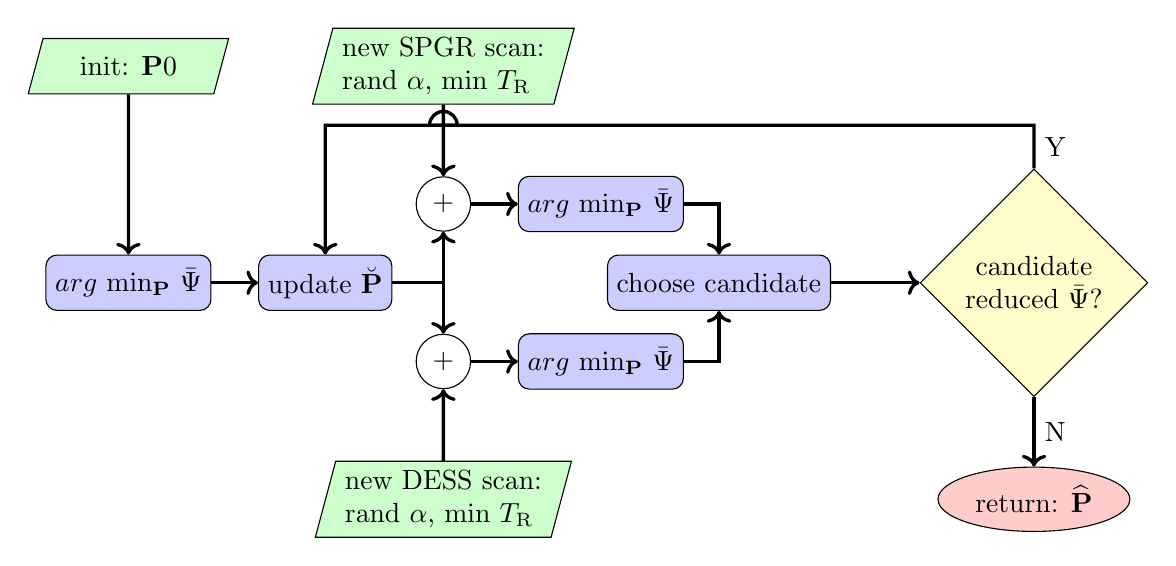
\begin{tikzpicture}[node distance=1em]
  
	% nodes
	\node[input] at (0,2.75) (start) 
		{\vwidth{6em}{init: $\iter{\bmP}{0}$}};
	\node[block] at (0,0) (opt0) 
		{$\argmin{\bmP} \expcost$};
	\node[block] at (2.5,0) (update) 
		{\vwidth{7em}{update $\bmPc$}};
	\node[sum] at (4,1) (sum1) {$+$};
	\node[sum] at (4,-1) (sum2) {$+$};
	\node[input] at (4,2.75) (spgr) 
		{\vwidth{8em}{new SPGR scan: rand $\flip$, min $\TR$}};
	\node[input] at (4,-2.75) (dess) 
		{\vwidth{8em}{new DESS scan: rand $\flip$, min $\TR$}};
	\node[block] at (6,1) (opt1) {$\argmin{\bmP} \expcost$};
	\node[block] at (6,-1) (opt2) {$\argmin{\bmP} \expcost$};
	\node[block] at (7.5,0) (opt3) {choose candidate};
	\node[decision] at (11.5,0) (comp) {candidate reduced $\expcost$?};
	\node[output] at (11.5,-2.75) (end) {return: $\est{\bmP}$};
	
	% connections
	\draw[arrow] (start) -- (opt0);
	\draw[arrow] (opt0) -- (update);
	\draw[arrow] (update) -| (sum1);
	\draw[arrow] (update) -| (sum2);
	\draw[arrow, name path=int1] (spgr) -- (sum1);
	\draw[arrow] (dess) -- (sum2);
	\draw[arrow] (sum1) -- (opt1);
	\draw[arrow] (sum2) -- (opt2);
	\draw[arrow] (opt1) -| (opt3);
	\draw[arrow] (opt2) -| (opt3);
	\draw[arrow] (opt3) -- (comp);
	\path[arrow, name path=int2] 
		(comp) -- node[name=yes, anchor=west]{Y} (11.5,2) -- (3,2) -- (update);
	\draw[arrow] (comp) -- node[name=no, anchor=west]{N} (end);
	
	% intersection
	\path[name intersections={of = int1 and int2}];
	\coordinate (S) at (intersection-1);
	\path[name path=circ] (S) circle(0.5em);
	\path [name intersections={of = circ and int2}];
	\coordinate (I1) at (intersection-1);
	\coordinate (I2) at (intersection-2);
	\draw[line] (comp) -- (11.5,2) -- (I2);
	\draw[arrow] (I1) -- (2.5,2) -- (update);
	\tkzDrawArc[color=black, very thick](S,I1)(I2);
  \end{tikzpicture}
  \caption{
	Block diagram of greedy scan profile construction.
	We set an original acquisition
	consisting of three SPGR and three DESS scans
	whose flip angles and repetition times 
	are respectively initialized randomly and minimally.
	We optimize the original acquisition subject to several constraints: 
	$\flip \in \brac{1,40}^\circ$ and $\TR\geq11.8$ms for SPGR; 
	$\flip \in \brac{1,60}^\circ$ and $\TR\geq17.5$ms for DESS;
	and $\sum_{d=1}^D \TRd \leq 263.7$ms
	(selected to allow 9 SPGR and 9 DESS scans
	each at minimal $\TR$,
	comparable to \cite{deoni:11:com}).
	We then seek to improve the acquisition 
	by appending another SPGR or DESS scan
	and repeating (constrained) optimization.
	This process iterates
	until additional scans no longer 
	improve estimation precision. 
  }
  \label{fig:mwf,schem}
\end{figure}

% since local opt, desirable to have good initialization
% however, unclear a priori how to best allocate scan time among init spgr/dess scans
% Fig diagrams greedy design approach... (ismrm abstract)
% idea is to first optimize a small scan profile
% only add scans as necessary
% solve sequence of opt problems
% note that while this approach not optimal, we can track quality of solution through coef of var cost
To this point,
we have only considered scan design
via acquisition parameter optimization
for a fixed combination 
of SPGR and DESS scans.
In single-component $\To,\Tt$ relaxometry
(studied in Section~\ref{s,scn-dsgn,opt}),
we were able to restrict 
our total scan time constraint
such that only three such scan profiles were feasible,
each of which we studied explicitly.
However in MWF imaging,
a greater number of datasets are required
for well-conditioned estimation
of a larger number of latent parameters.
To permit scan profiles
with greater numbers of datasets,
we must optimize with respect
to a larger time constraint
that allows combinatorially many more scan profiles.
As an alternative
to exhaustively comparing all scan profiles
(that too, only via local optima),
we employ a greedy method 
for scan profile construction,
diagrammed in Figure~\ref{fig:mwf,schem}.
We first optimize
an initial scan profile consisting 
of only $3$ SPGR and $3$ DESS scans.
We then seek 
to improve the acquisition 
by appending another SPGR or DESS scan
to the previously optimized scan profile
and repeating constrained optimization.
If we find
that at least one appended scan profile
reduces the objective 
while meeting all constraints,
we update the previous scan profile
with the appended scan profile
that better improved the objective
and repeat the process. 
Otherwise, 
we return the previously optimized scan profile.
Observe that while this approach
is far from optimal,
we can easily assess solution quality 
via expected $\ff$ relative standard deviation 
$\sqrt{\expcost(\est{\bmP})}$.

\begin{table}[!tb]
  \centering
  \begin{tabular}{r | c | c}
    \hline
    \hline
    & Optimized flip angles (deg) & Optimized repetition times (ms) \\
    \hline
    SPGR & $[38.1,12.9,9.2,33.5]^\mathsf{T}$ & $[50.2,32.4,16.4,11.8]^\mathsf{T}$ \\
    DESS & $[32.0,40.3,52.9]^\mathsf{T}$ & $[17.5,98.0,37.6]^\mathsf{T}$ \\
    \hline
    \hline
  \end{tabular}
  \caption{
		SPGR/DESS flip angles and repetition times
		that comprise $\est{\bmP}$,
		a scan parameter designed
		for precise $\ff$ estimation in WM
		via the sequence of optimization problems
		described in Figure~\ref{fig:mwf,schem}. 
		For our noise variance measurements,
		this acquisition is expected
		to yield $28.5$\% relative standard deviation
		in asymptotically unbiased $\ff$ estimates
		from two-compartment
		SPGR \eqref{eq:mwf,spgr,mod-exchg0}
		and DESS \eqref{eq:mwf,dess-def,mod-exchg0}-\eqref{eq:mwf,dess-ref,mod-exchg0}
		signal models.
		Remarkably, 
		this optimized scan profile involving $\TR$ variation
		achieves better $\ff$ estimation precision
		than a similarly optimized scan profile
		with fixed minimum-$\TR$ acquisitions,
		even though the latter 
		can utilize many more scans 
		for the given time budget.
  }
  \label{tab:mwf,acq}
\end{table}

% Table shows resulting optimized scan parameters
% these parameters have rstd of 0.2853 (reduced from 1.1508)
% time of 64s
% using fmincon with tolFun and tolX of 10^-7 and maxIter 500 for each opt
% hardware info, etc 
% using (9,9) got about 0.3873 rstd 
% tr variation does seem to help!
Table~\ref{tab:mwf,acq} summarizes
the optimized scan parameter $\est{\bmP}$ 
that arises
from one representative realization 
of our scan profile construction procedure.
Using \texttt{fmincon} 
in \matlab R2013a
for each inner-step optimization
(with the ``active set'' option and
with an objective function convergence tolerance of $10^{-7}$),
this realization took 64s run time
on a 3.5GHz desktop computer with 32GB RAM.
We find that $\sqrt{\expcost(\est{\bmP})} = 0.285$, 
meaning that at a realistic noise level,
the SPGR/DESS acquisition defined by $\est{\bmP}$
is expected to yield $28.5$\% relative standard deviation
in asymptotically unbiased $\ff$ estimates
from SPGR \eqref{eq:mwf,spgr,mod-exchg0} 
and DESS 
\eqref{eq:mwf,dess-def,mod-exchg0}-\eqref{eq:mwf,dess-ref,mod-exchg0}
non-exchanging two-compartment signal models.

Interestingly,
we observe empirically
that the above scan profile construction procedure
tends to append far fewer additional scans
than is possible under our time budget: 
here, it halts at a small scan profile
consisting of only 4 SPGR and 3 DESS scans. 
We investigated this phenomenon further
by repeating the above procedure
under the same time constraint,
but now initializing with a profile
consisting of $9$ SPGR and $9$ DESS scans
whose repetition times are implicitly restricted
to be minimal. 
Over many random flip angle initializations,
we found after optimization
that this expanded minimum-$\TR$ scan profile could achieve
an expected $\ff$ relative standard deviation
no better than $0.387$,
suggesting that $\TR$ variation 
across scans is important 
for building scan profiles
that permit precise $\ff$ estimation.

%%%%%%%%%%%%%%%%%%%%%%%%%%%%%%%%%%%%%%%%%%%%%%%%%%%
\section{Experimentation}
\label{s,mwf,exp}
%%%%%%%%%%%%%%%%%%%%%%%%%%%%%%%%%%%%%%%%%%%%%%%%%%%

% maybe repeat some details from ch 4
% krr details
% preliminary image

%%%%%%%%%%%%%%%%%%%%%%%%%%%%%%%%%%%%%%%%%%%%%%%%%%%
\section{Summary and Future Work}
\label{s,mwf,summ}
%%%%%%%%%%%%%%%%%%%%%%%%%%%%%%%%%%%%%%%%%%%%%%%%%%%

\todo{discuss negative $\ff$ range}


\chapter{Future~Work}
\label{c,future}
% concluding remarks

This chapter suggests avenues
for further QMRI research,
focusing on relatively broad future directions
that this thesis has not explored.
Discussion sections
within main body chapters
offer more focused ideas 
for topic-specific extensions,
whereas the appendices organize 
partially investigated but still immature topics
that are less related to QMRI.

%%%%%%%%%%%%%%%%%%%%%%%%%%%%%%%%%%%%%%%%%%%%%%%%%%%
\section{Combining PERK with Image Reconstruction}
\label{s,future,recon}
%%%%%%%%%%%%%%%%%%%%%%%%%%%%%%%%%%%%%%%%%%%%%%%%%%%

This thesis has considered parameter estimation
to be separate from image reconstruction.
This separation affords fast data processing
but may leave room for improved estimation performance,
especially when raw data is undersampled.
One could instead seek 
to estimate parameters 
directly from raw data.
One simple approach 
to combining image reconstruction
with PERK-based estimation
might seek to solve
the joint optimization problem
\begin{align}
	\paren{\est{\bmX},\est{\bmY},\est{\bmh},\est{\bmb}} &\in \set{%
		\argmin{%
			\substack{%
				\bmX \in \complexes{L \times V} \\
				\bmY \in \complexes{D \times V} \\
				\bmh \in \hilb^L \\
				\bmb \in \complexes{L}
			}%
		}%
		\costa{\bmh,\bmb} 
			+ \beta_1 \frob{\bmD-\bmY\bmA}^2 
			+ \beta_2 \sum_{v=1}^V \norm{\bmh\paren{\bmy_v,\bmnu_v}+\bmb-\bmx_v}^2_2
	},
	\label{eq:future,recon}
\end{align}
where 
$\bmX := \brac{\bmx_1,\dots,\bmx_V} \in \complexes{L \times V}$
and
$\bmY := \brac{\bmy_1,\dots,\bmy_V} \in \complexes{D \times V}$
respectively collect $L$ latent parameters 
and $D$ image datasets 
at $V$ voxels;
$\bmh : \complexes{D+N} \mapsto \complexes{L}$ 
and $\bmb \in \complexes{L}$ 
together denote a PERK-like regression function with offset;
$\Psi$ is the PERK cost function \eqref{eq:perk,cost};
$\bmD \in \complexes{D \times K}$
collects $D$ raw datasets 
each acquired with $K$ samples;
$\bmA \in \complexes{V \times K}$ 
denotes the MRI system model;
$\bmnu_v$ denotes a known parameter at the $v$th voxel;
and $\beta_1,\beta_2$ are free parameters
that balance cost function terms.
Here, 
estimator fidelity to training points
and image fidelity to raw data
are respectively enforced 
by the first and second cost function terms,
while the third term entangles image reconstruction
and parameter estimation.

For continuously differentiable kernels,
\eqref{eq:future,recon} is amenable 
to iterative local optimization 
via alternating minimization.
One simple algorithm iterates
the following updates:
\begin{align}
	\paren{\iter{\bmh}{t},\iter{\bmb}{t}} &\gets
		\argmin{%
			\substack{%
				\bmh \in \hilb^L \\
				\bmb \in \complexes{L}
			}%
		}%
		\costa{\bmh,\bmb}	+ \beta_2 \sum_{v=1}^V \norm{%
			\bmh\paren{\iter{\bmy}{t-1}_v,\bmnu_v}+\bmb-\iter{\bmx}{t-1}_v
		}^2_2%
		\label{eq:future,hb-update} 
		\\
	\iter{\bmY}{t} &\gets
		\argmin{%
			\bmY \in \complexes{D \times V}
		}%
		\frob{\bmD-\bmY\bmA}^2 + 
			\frac{\beta_2}{\beta_1} \sum_{v=1}^V \norm{%
				\iter{\bmh}{t}\paren{\bmy_v,\bmnu_v}+\iter{\bmb}{t}-\iter{\bmx}{t-1}_v
			}^2_2%
		\label{eq:future,Y-update}		
		\\
	\iter{\bmX}{t} &\gets
		\brac{%
			\iter{\bmh}{t}\paren{\iter{\bmy}{t}_1,\bmnu_1}+\iter{\bmb}{t},
			\dots,
			\iter{\bmh}{t}\paren{\iter{\bmy}{t}_V,\bmnu_V}+\iter{\bmb}{t}
		}%
		\label{eq:future,X-update}			
\end{align}
where $\iter{\paren{\cdot}}{t}$ denotes the $t$th iterate.
Regression function update \eqref{eq:future,hb-update}
adaptively retrains 
using prior iterate per-voxel triples
$\paren{\iter{\bmx}{t-1}_v,\bmnu_v,\iter{\bmy}{t-1}_v}$
for $v \in \set{1,\dots,V}$
as additional training points.
Image update \eqref{eq:future,Y-update}
enforces consistency 
not only with data
but also with latent parameter iterates
(via regression function iterates).
Latent parameter update \eqref{eq:future,X-update}
evaluates the current regression function iterate
at the current image iterate.
Though it does require kernel gradients,
observe that solving \eqref{eq:future,recon}
does not require signal model gradients
and thus \eqref{eq:future,recon} or similar variations 
may be useful even when analytical signal models
are cumbersome or altogether unavailable.
 
%%%%%%%%%%%%%%%%%%%%%%%%%%%%%%%%%%%%%%%%%%%%%%%%%%%
\section{Exploiting Off-Resonance for Myelin Water Imaging}
\label{s,future,off-res}
%%%%%%%%%%%%%%%%%%%%%%%%%%%%%%%%%%%%%%%%%%%%%%%%%%%

Though early sections in Chapter~\ref{c,mwf} 
provided a simple model  
of off-resonance distribution variation 
across intravoxel compartments,
experiments therein 
ultimately used simpler magnitude signal models
that neglected off-resonance effects.
However,
off-resonance distributions
do often differ significantly 
across compartments
in cerebral tissue \cite{miller:10:aot-1,miller:10:aot-2},
so accounting for compartment-specific off-resonance effects
could aid in better distinguishing compartments
and could thereby enable further-improved myelin water imaging.
For designing off-resonance-informed myelin water imaging acquisitions,
it is reasonable
to consider pulse sequences
whose acquisition parameters
can strongly influence signal sensitivity 
to off-resonance effects.
In this respect,
the small-tip fast recovery (STFR) sequence \cite{nielsen:13:stf}
may be well-suited for off-resonance-informed myelin water imaging
because its tip-up pulse magnitude and phase
provide additional degrees of freedom
by which to sensitize acquisitions
to compartmental off-resonance effects.
Off-resonance-informed myelin water imaging
using (spoiled) STFR sequences
is an active area of research 
in our group.

%%%%%%%%%%%%%%%%%%%%%%%%%%%%%%%%%%%%%%%%%%%%%%%%%%%
\section{Correlating with Other Myelin Biomarkers}
\label{s,future,myelin}
%%%%%%%%%%%%%%%%%%%%%%%%%%%%%%%%%%%%%%%%%%%%%%%%%%%

As discussed in Section~\ref{s,mwf,disc},
fundamental differences 
between DESS $\ff$ and MESE MWF imaging
may limit their quantitative comparability.
To build evidence 
that DESS $\ff$ imaging
is nevertheless a specific biomarker
for intact myelin content,
we are also interested 
in how $\ff$ correlates 
with other myelin biomarkers.
One contending noninvasive marker arises
from MR pulse sequences sensitized
to the inhomogeneous magnetization transfer (ihMT) effect
\cite{varma:15:mtf},
which has recently been shown
to be specific
to the large membrane lipids
that comprise much of myelin
\cite{varma:15:iom, swanson:17:mda}.
Multi-compartmental and ihHT MRI markers 
could be successively compared 
through \exvivo, healthy volunteer, and patient studies.
Outside MRI,
invasive measurements
from histology
have been used to study myelin 
(as in \eg, \cite{gareau:00:mta, webb:03:imt})
and could serve as a gold-standard \insitu marker.
MRI and histological markers
could be compared 
by correlating respective \exvivo and \insitu studies.


% appendix
\appendix

\chapter{Multiple-Dataset Complex Coil Combination}
\label{a,cc-multi}
% appendix: sense with multiple datasets

In the completed thesis,
this appendix will describe 
an unpublished algorithm
for combining multiple MRI datasets
when each dataset is acquired 
using multiple receiver coils
with fixed coil geometry.
Such sequences of coil datasets arise naturally
in many quantitative MRI applications,
including the ones studied
in Chapters~\ref{c,scn-dsgn}-\ref{c,krr}.
The algorithm extends \cite{ying:07:jir}
(which considers joint image reconstruction
and coil sensitivity estimation
in the case of a single dataset)
to exploit the fixed coil sensitivity 
across several datasets,
thereby improving estimation conditionality
as compared to separate coil combination
across datasets. 


\chapter{SS-Informed RF Pulse Design}
\label{a,ss-rf}
% steady-state rf pulse design



%\chapter{Diffusive Signal Loss in DESS}
%\label{a,dess-diff}
%% diffusive signal loss in dess

In the completed thesis,
this appendix will present
an unpublished analysis
of model mismatch 
in single-compartment DESS signal models 
\eqref{eq:dess-def-model} and \eqref{eq:dess-ref-model}
in the presence of diffusion.
We first develop models
that describe the single-compartment DESS signal 
in the presence of diffusion.
We then use these models
to show through phantom experiments
that neglecting diffusive effects
during $\Tt$ estimation
(as in Chapters~\ref{c,relax}-\ref{c,scn-dsgn})
induces significant estimation bias.
We conclude with recommendations
for MR acquisition settings
(specifically, for dephasing gradient area)
that reduce diffusion-related estimation bias
without excessively imparting other bias.
These recommendations were used 
to guide DESS acquisition design
for all relevant experiments
considered in the main body of this thesis.


% bibliography
\bibliographystyle{ieeetr}
\bibliography{../bib/master.bib}

\end{document}
